%###################################################################################%
%
%Startdatei fuer den Praxisprojektbericht%
%
%###################################################################################%

%###################################################################################################
%
%Style für eine Abschlussarbeit an der Ostfalia - Hochschule für angewandte
% Wissenschaften
%
%###################################################################################################

%Schriftgroesse, Layout, Papierformat, Art des Dokumentes
\documentclass[%
	a4paper,			% Papierformat
	oneside,			% einseitiger Druck
	%twoside,			% zweiseitiger Druck
	12pt,				% Schriftgröße
	onecolumn,			% einspaltiger Text
	%twocolumn,			% zweispaltiger Text
	openright,			% Kapitel dürfen nur auf einer rechten Seite beginnen
	openany,			% Kapitel dürfen rechts oder links beginnen
	parskip=half,		% eine halbe Zeile Abstand zw. Absätzen
	headsepline,		% Kopfzeilenlinie
	footsepline,		% Fußzeilenlinie
	bibliography=totoc,	% Bibliographie im Inhaltsverzeichnis
	%idxtotoc			% Index im Inhaltsverzeichnis
	]{scrbook}

\usepackage[utf8]{inputenc}	
	
%Einstellungen der Seitenraender
\usepackage[
	left=30mm,
	right=20mm,
	top=45mm,
	bottom=55mm,
	%includeheadfoot,
	]{geometry}

%Fuer Zeilenabstand
\usepackage{setspace}

% deutsche Silbentrennung etc.
\usepackage[ngerman]{babel}

% Grafiken: PDF, GIF, PNG
\usepackage{graphicx}

%Stichwortverzeichnis/Index erstellen
\usepackage{makeidx}
\usepackage[
acronym, %Abkürzungsverzeichnis
toc]%Einträge im Inhaltsverzeichnis
{glossaries}
	\makeindex
	\makeglossaries

%Schriftart auf Helvetica umstellen (aehnlich Arial unter Windows)
\usepackage{helvet}
\renewcommand{\familydefault}{\sfdefault}

%Sammelsurium
\usepackage[T1]{fontenc} 
\usepackage[hyphens]{url}
\usepackage{capt-of}
\usepackage{listings}
\usepackage{epsfig}

%Richten den Absatz nach links aus (wird nicht bei Bachelorthesis benoetigt)
\setlength{\parindent}{0pt} 

% Fortlaufende Kapitelüberschriften in der Kopfzeile
\pagestyle{headings}

\usepackage{scrpage2}
\pagestyle{scrheadings}
\setkomafont{pageheadfoot}{\normalfont\bfseries}
\renewcommand*\chapterpagestyle{scrheadings}
\renewcommand*\sectionmark[1]{\markright{\thesection\ #1}} 
\cfoot{}
\ofoot{\pagemark}

% Stil des Literaturverzeichnis
\bibliographystyle{alphadin}
%\setbibpreamble{Beispielsweise Hinweis zur Sortierung des
%Literaturverzeichnisses.\par\bigskip}

%PDF-Dateien einbinden
\usepackage{pdfpages}

%Groesse der Kopfzeile veraendern
\addtolength{\headheight}{1.6pt}

%Kapitelname aendern
\renewcommand\lstlistlistingname{Quellcodeverzeichnis}

%Abkuerzungsverzeichnis
\usepackage{nomencl}
	\let\abbrev\nomenclature
	\renewcommand{\nomname}{Abkuerzungsverzeichnis}
	\setlength{\nomlabelwidth}{.25\hsize}
	\renewcommand{\nomlabel}[1]{#1\dotfill}
	\setlength{\nomitemsep}{-\parsep}

\usepackage[normalem]{ulem}
	\newcommand{\markup}[1]{\uline{#1}}
\makenomenclature

% erweiterte Tabellen
\usepackage{array}

%Pfeile usw. einfuegen
\usepackage{amsmath}

%fuer Ueberschriften > 4 Eintraege
\setcounter{secnumdepth}{5}	%nummerierung im Text
\setcounter{tocdepth}{3}	%nummerierung im Inhaltsverzeichnis

% Farben
\usepackage{color}
\definecolor{LinkColor}{rgb}{0,0,0.6}
\definecolor{ListingBG}{rgb}{0.9,0.9,0.9}

%fuer mehrzeilige Kommentare
\newcommand{\comment}[1]{}

%fuer einen neuen Absatz ohne Einrueckung mit einfachen Zeilenabstand
\newcommand{\newpassage}{\hspace{1em}\vspace{1.0em}\\}

%fuer einen neuen Absatz mit Einrueckung mit einfachen Zeilenabstand
\newcommand{\newpassageL}{\hspace{1em}\vspace{1.0em}\\ \hspace*{5mm}}

%fuer das Zitieren aus einer bib-Datei
%\usepackage[round]{natbib}
%\usepackage{biblatex} %wegen textcite nehmen wollen

% Indirektes Zitieren
\newcommand{\citeindirect}[2]{
(Vgl. \cite{#1}, S. {#2})
%\footnote{Vgl. \cite{#1}, S. {#2}.}
%\footnote{Vgl. \citeauthor{#1} (\citeyear{#1}), S. #2.}
}

% direktes Zitieren
\newcommand{\citedirect}[2]{
(\cite{#1} , S. #2)
%\footnote{\cite{#1} , S. #2.}
%\footnote{\citeauthor{#1} (\citeyear{#1}), S. #2.}
}

% Zitieren einer Abbildung
\newcommand{\citeabb}[2]{
\citeauthor{#1} (\citeyear{#1}), S. #2.
}

% Zitieren einer Quelle aus dem Internet
\newcommand{\citeinternet}[2]{
\footnote{Vgl. \citeauthor{#1} (\citeyear{#1}), S. #2.}
}

\newcommand{\tocite}[1]{
\footnote{Vgl. \cite{#1}}
}

%EDIT command
\newcommand{\editHere}[1]{\textbf{\textcolor{red}{[BEARBEITEN: \MakeUppercase{#1}]}}}

\usepackage{boxedminipage}

%Eurozeichen
\usepackage{eurosym}

%Komprimierung von Text und Grafiken, 0=keine 9=hoechste
\pdfcompresslevel=0

% Hyperlinks (anklickbar im PDF)
\usepackage[%
    pdftitle={Titel der Arbeit},%
    pdfauthor={Vorname Nachname},%
    pdfpagemode=UseOutlines
]{hyperref}   

\hypersetup{%
    colorlinks=true,%    farbige Links statt Rahmen
    breaklinks=true,
    linkcolor=LinkColor,
    citecolor=LinkColor,
    filecolor=LinkColor,
    menucolor=LinkColor,
    urlcolor=LinkColor,
    }

%Für die optimsche Gestaltung der Java-Code-Listings
%\lstset{language=Java,numbers=left,numbersep=5pt,tabsize=4,basicstyle=\small,extendedchars=true,flexiblecolumns=true,frame=tb}
\definecolor{dkgreen}{rgb}{0,0.6,0}
\definecolor{gray}{rgb}{0.5,0.5,0.5}
\definecolor{mauve}{rgb}{0.58,0,0.82}

\lstset{frame=tb,
  language=Java,
  aboveskip=3mm,
  belowskip=3mm,
  showstringspaces=false,
  columns=flexible,
  basicstyle={\small\ttfamily},
  numbers=none,
  numberstyle=\tiny\color{gray},
  keywordstyle=\color{blue},
  commentstyle=\color{dkgreen},
  stringstyle=\color{mauve},
  breaklines=true,
  breakatwhitespace=true,
  tabsize=3
}

% Definition eigener Operatoren (im Header)
\DeclareMathOperator{\rg}{Rang}

%Flowcharts
\usepackage{tikz}
\usepackage{pgf-umlsd}
\usepgflibrary{arrows}
\usetikzlibrary{shapes,arrows}
\usetikzlibrary{shapes.multipart}
\usetikzlibrary{matrix}
\usetikzlibrary{positioning}
\usetikzlibrary{shadows}
\usetikzlibrary{calc}

% Define block styles
\tikzstyle{decision} = [diamond, draw, fill=white!20, 
    text width=4.5em, text badly centered, node distance=3cm, inner sep=0pt, general shadow={
                shadow xshift=0.0625in,
                shadow yshift=-0.0625in,
                opacity=0.5,
                fill=black!50
            }]
\tikzstyle{block} = [rectangle, draw, fill=white!20, 
    text width=5em, text centered, rounded corners, minimum height=2em, general shadow={
                shadow xshift=0.0625in,
                shadow yshift=-0.0625in,
                opacity=0.5,
                fill=black!50
            }]
\tikzstyle{line} = [draw, -latex']
\tikzstyle{cloud} = [draw, ellipse,fill=black!20, node distance=3cm, text centered, 
    minimum height=2.5em,  text width=2em,
general shadow={
                shadow xshift=0.0625in,
                shadow yshift=-0.0625in,
                opacity=0.5,
                fill=black!50
            }]
\tikzstyle{placeholder} = [draw, rectangle,fill=white!20, color=white, text=black,
    minimum height=2.5em,  text width=2em, node distance=1.5cm
]
\tikzstyle{kasten} = [draw, rectangle, thick, dashed,
    text width=15.15cm, minimum height=2cm, node distance=2cm
]
\tikzstyle{database} = [
  draw,
      cylinder,
      cylinder uses custom fill,
       fill=white!20, 
      shape border rotate=90,
      aspect=0.25,
  minimum height=3em, minimum width=2.5em,
general shadow={
                shadow xshift=0.0625in,
                shadow yshift=-0.0625in,
                opacity=0.5,
                fill=black!50
            }
]
\tikzstyle{kreis} = [ellipse, thick, draw, dashed, minimum height=4.8cm,  text width=7.2cm, fill=black!5
]

%db notation
\makeatletter
\pgfarrowsdeclare{crow's foot}{crow's foot}
{
  \pgfarrowsleftextend{+-.5\pgflinewidth}%
  \pgfarrowsrightextend{+.5\pgflinewidth}%
}
{
  \pgfutil@tempdima=0.5pt%
  \advance\pgfutil@tempdima by.25\pgflinewidth%
  \pgfsetdash{}{+0pt}%
  \pgfsetmiterjoin%
  \pgfpathmoveto{\pgfqpoint{0pt}{-6\pgfutil@tempdima}}%
  \pgfpathlineto{\pgfqpoint{-6\pgfutil@tempdima}{0pt}}%
  \pgfpathlineto{\pgfqpoint{0pt}{6\pgfutil@tempdima}}%
  \pgfusepathqstroke%
}

\tikzset{
    entity/.code={
        \tikzset{
            label=above:#1,
            name=#1,
            inner sep=0pt,
            every entity/.try,
            fill=white,
            general shadow={
                shadow xshift=0.0625in,
                shadow yshift=-0.0625in,
                opacity=0.5,
                fill=black!50
            }
        }%
        \def\entityname{#1}%
    },
    entity anchor/.style={matrix anchor=#1.center},
    every entity/.style={
            draw,
    },
    every property/.style={
        inner xsep=0.25cm, inner ysep=0.125cm, anchor=west, text width=10em
    },
    zig zag to/.style={
        to path={(\tikztostart) -| ($(\tikztostart)!#1!(\tikztotarget)$) |- (\tikztotarget)}
    },
    zig zag to/.default=0.5,
    one to many/.style={
        -crow's foot, zig zag to
    },
    many to one/.style={
        crow's foot-, zig zag to
    },
    many to many/.style={
        crow's foot-crow's foot, zig zag to
    }
}
\def\property#1{\node[name=\entityname-#1, every property/.try]{#1};}
\def\properties{\begingroup\catcode`\_=11\relax\processproperties}
\def\processproperties#1{\endgroup%
    \def\propertycode{}%
    \foreach \p in {#1}{%
        \expandafter\expandafter\expandafter\gdef\expandafter\expandafter\expandafter\propertycode%
            \expandafter\expandafter\expandafter{\expandafter\propertycode\expandafter\property\expandafter{\p}\\}%
    }%
    \propertycode%
}
\newglossaryentry{falkofx} {
	name=FalkoFX,
	description={Eine Anwendung zur Visualisierung von länderspezifischen Fahrzeugdaten}
}

\usepackage{listings}
\usepackage{float}
\usepackage{subfig}
\usepackage{csquotes}
\usepackage{needspace}

\hyphenchar\font=\string"7F
\hyphenation{Stream Streams Ge-ne-ric-Re-sult-Ta-ble-Con-trol-lers}

\newcommand{\heading}[1]{\needspace{4\baselineskip}\textbf{#1}\par}


%########Dokument###################################################################%

\begin{document}

\frontmatter
% Titelseite
%########Titelseite###################################################################################%

\begin{titlepage}

	\thispagestyle{empty}
	
	\begin{minipage}{2.1cm}
		
\includegraphics[width=2cm]{grafiken/fh_logo_klein.jpg}
	\end{minipage}
	\begin{minipage}{10.0cm}
		Ostfalia - Hochschule für angewandte Wissenschaften\\
		Fachbereich Informatik\\
		Studiengang Informatik\\
		Vertiefungsrichtung Software-Engineering
	\end{minipage}

	\vspace{15mm}

	\begin{center}
		\LARGE \textbf{User-Experience Optimierung \\ in einer JavaFX-Anwendung\\[10mm]}
	\end{center}
	
	\begin{center}
		\normalsize Bachelorarbeit\\[1cm]
		Zur Erlangung des Grades eines Bachelor of Science\\ 
		der Fakultät Informatik\\
		der Ostfalia - Hochschule für angewandte Wissenschaften\\[10mm]
	\end{center}

	\begin{table}[h]
		\centering
		\hspace{50mm}\begin{tabular}{lcl}
			eingereicht bei &  & Erstprüfer: Prof. Dr. Bernd Müller\\
			& & Zweitprüfer: Dennis Schladebeck (B. Sc.) \\
			& & \\
			von & & Jan Philipp Wiegmann\\
			& & Kruppstraße 18\\
			& & 38126 Braunschweig\\
			& & Mat.-Nr. 70312216\\
		\end{tabular}
	\end{table}

	\vspace{20mm}

	\begin{table}[h]
		\begin{tabular}{lll}
			Braunschweig, den \today\\
		\end{tabular}
	\end{table}

\end{titlepage}

%*******************************************************************************
%                                                                              *
%                 Datei: erklaerung.tex                                        *
%                                                                              *
%                 Stand: 30.10.2013,17.03.14   14.36 Uhr   (Elt,Se)            *
%                                                                              *
%*******************************************************************************

\section*{Erkl"arung}
{\large\textsf{Hiermit versichere ich, dass ich die vorliegende Arbeit 
   selbst"andig verfasst und keine anderen als die angegebenen Quellen und 
   Hilfsmittel benutzt habe. Ich versichere, dass ich alle w"ortlich oder 
   sinngem"a"s aus anderen Werken "ubernommenen Aussagen als solche gekennzeichnet
   habe, und dass die eingereichte Arbeit weder vollst"andig noch in wesentlichen
   Teilen Gegenstand eines anderen Pr"ufungsverfahrens gewesen ist.
   \vspace*{3em}\\
   \underline{\ \ \ \ \ \ \ \ \ \ \ \ \ \ \ \ \ \ \ \ \ \ \ \ \ \ \ \ \ \ \ \ \ 
              \ \ \ \ \ \ \ \ \ \ \ \ \ \ \ \ \ \ \ \ \ \ \ \ \ \ \ \ \ \ \ \ \ 
              \ \ \ \ \ \ \ \ \ \ \ \ \ \ \ \ \ \ \ \ \ \ \ \ \ \ \ \ \ }\\[1.0ex]
   Ort, Datum \hspace{5cm} Unterschrift}}

\thispagestyle{empty}
\section*{Abstract}

\tableofcontents

\mainmatter
\chapter{Einleitung}
\section{Ziele der Arbeit} \label{sec:einlZiel}

\section{Motivation} \label{sec:einlMotivation}

\section{Aufbau der Arbeit} \label{sec:einlAufbau}

\chapter{Grundlagen}
\section{Usability}
\textit{Usability} in der Software-Entwicklung ist ein Qualitätsmaß, anhand dessen eine Einschätzung über die Einfachheit der Bedienung einer Benutzeroberfläche ermöglicht wird \cite{Nielsen2012}. Umgangssprachlich wird der Begriff \enquote{Benutzerfreundlichkeit} als deutsches Synonym verwendet. Betrachtet man jedoch den Wortstamm genauer, bemerkt man, dass die englische Vokabel aus zwei einzelnen Wörtern besteht. Dies ist zum einen \enquote{use} (engl. benutzen) und zum anderen \enquote{ability} (engl. die Möglichkeit). 

Nach Nielsen wird die Qualität einer Anwendung hinsichtlich der Usability durch 5 Kernaspekte bestimmt:
\begin{itemize}
	\item Erlernbarkeit
	\item Effizienz
	\item Einprägsamkeit
	\item Fehlertoleranz
	\item Zufriedenheit \cite{Nielsen2012}
\end{itemize}
Alle diese Aspekte können zu einer guten Gebrauchstauglichkeit beitragen. Eine hohe Erlernbarkeit ist gegeben, wenn der Dialog zwischen der Maschine und dem Anwender einfach gestaltet ist, sodass die Bedienung schnell erlernt werden kann. Es ist hilfreich, Designkonzepte zu verwenden, die dem Anwender aus anderen Anwendungen oder aus der Natur vertraut sind \cite[Learnability]{UsabilityFirstGlossary}. Auch die Erfüllung psychologischer Grundsätze (siehe Kap. \ref{sec:uxdPsychology} und Kap. \ref{sec:uidRules}) ist ein wichtiger Faktor. Ein effizienter Dialog erlaubt es dem Nutzer, seine Ziele möglichst schnell zu erreichen. Kurze Ladezeiten und wenige zur Problemlösung benötigte Interaktionen fördern die Effizienz. Einprägsam ist eine Software, wenn ein Nutzer nach längerer Nicht-Benutzung dieser, ohne viel Zeitaufwand, den professionellen Umgang damit wieder erlernen kann \cite{Nielsen2012}. Bei der Fehlertoleranz geht es darum, dass die Anwendung fehlerhafte Eingaben erkennt und behandeln kann. Entweder kann die Anwendung den Fehler kompensieren und bereinigen oder der Nutzer muss über die Fehleingabe informiert werden und die Gelegenheit bekommen, korrekte Eingaben zu machen. Da bei der Usability stets der Nutzer im Fokus der Entwicklung steht, ist es von entscheidender Bedeutung, diesen zufrieden zu stellen. Ein gutes Design, das eine angenehme Bedienung ermöglicht, hilft dabei \cite{Nielsen2012}. \par

\section{User-Experience Design} \label{sec:uxd}
Der Begriff \textit{User-Experience} (kurz: UX) beschreibt das Nutzungsempfinden einer Person, wenn Sie mit einem System interagiert. Der Ausdruck ist meist im Bereich der Mensch-Computer-Interaktion vorzufinden, beschränkt sich aber nicht auf diesen. \cite{Gube2010} So kann der Begriff auch auf andere Produkte, wie z.B. Mikrowellen, Brettspiele oder ganze Produktreihen (vgl. Microsoft Office Produkte) angewandt werden. Im Rahmen dieser Arbeit wird jedoch nur der Teilbereich der Mensch-Computer-Interaktion im Rahmen einer einzelnen Anwendung betrachtet. \par
Im Gegensatz zur Usability berücksichtigt die UX die Erwartungshaltung des Nutzers und versucht, ein angenehmes Gesamtbild der Anwendung und der Interaktion mit dieser zu vermitteln. Das Ziel des User-Experience Designs ist es nicht nur, eine hohe Produktivität zu ermöglichen, vielmehr versucht sie, die Interaktion zu einem Erlebnis zu machen, das dem Anwender positiv in Erinnerung bleibt. Dies geht sogar so weit, dass der UX-Designer beschließt, dem Nutzer unter Umständen Funktionalitäten vorzuenthalten, um das Erlebnis zu sichern \cite{Thielsch2015}. Als Beispiel führt Thielsch den \textit{Drift-Table} an. Bei dem Drift-Table handelt es sich um einen niedrigen Couchtisch, in dem ein Bildschirm eingebaut wurde, der Luftaufnahmen von Großbritannien zeigt. Durch Kraftausübung an den Kanten des Tisches kann über das Land mit einer mäßigen Maximalgeschwindigkeit (50 km/h) \enquote{gereist} werden. Obwohl sich viele Nutzer gewünscht haben, direkt zu einem Ort springen zu können, hat sich der Erfinder bewusst dagegen entschieden, um das Erlebnis zu wahren \cite{Thielsch2015}. \par

\subsection{Interaktionsdesign} \label{sec:interactionDesign}
Ein Teilgebiet des UX-Designs ist das Interaktionsdesign (kurz: IxD). Der Fachbereich beschäftigt sich konkret mit den Schnittstellen, die ein Computersystem zwischen der Maschine und dem Nutzer bietet. Über diese Eingabe- und Ausgabesysteme können Informationen in beide Richtungen ausgetauscht werden.\par
Dafür muss der Benutzer sich zunächst darüber im Klaren sein, welches Ziel er mithilfe der ihm gegebenen technischen Möglichkeiten verfolgt. Er überlegt sich Handlungsschritte, von denen er glaubt, dass sie ihn zu seinem Ziel führen. Bei der Ausführung dieser, interagiert er mit dem Computersystem, welches die Eingaben verarbeitet und die Anwendung in einen neuen Zustand überführt. Dieser neue Zustand, der sich z.B. in einer Änderung der grafischen Oberfläche bemerkbar macht, wird von dem Nutzer interpretiert, woraufhin dieser einen weiteren Handlungsschritt ausführt. Dies tut er solange bis er seine Zielsetzung erreicht hat \cite{Ullenboom2014}. Daraus ergibt sich das Konzept einer Interaktion. \enquote{Das Ziel des Interaktionsdesigns ist es nun, diese Interaktion so zu gestalten, dass der Benutzer möglichst effizient, effektiv und zufriedenstellend an seine Ziele kommt\cite[S. 122]{Ullenboom2014}}.\par
Ein konkretes Beispiel ist das Ausdrucken eines Dokumentes in Schwarz-Weiß. Der Nutzer wählt aus dem Menü den Befehl \textit{Drucken} aus. Daraufhin öffnet sich ein Fenster, in dem die Einstellungen spezifiziert werden müssen. Der Anwender bekommt diese visuelle Änderung mit und überlegt sich, wo er welche Einstellungen ändern kann. Er wählt in der aktuellen Ansicht den zu verwendenden Drucker aus und betätigt daraufhin die Schaltfläche zum Verwalten der Druckereinstellungen. In dem weiteren Fenster kann er nun die Farbe auf Schwarz-Weiß stellen. Er bestätigt die Änderung und sendet danach den Druckauftrag ab. Werden keine Fehler festgestellt, ist damit die Interaktion abgeschlossen.\par
Donald A. Norman entwickelte ein Modell, das eben diese Interaktion abbildet. Es besteht aus 7 Phasen, die der Nutzer durchläuft, wenn er mit einem System interagiert. \par
\begin{figure}[H]
 \centering
 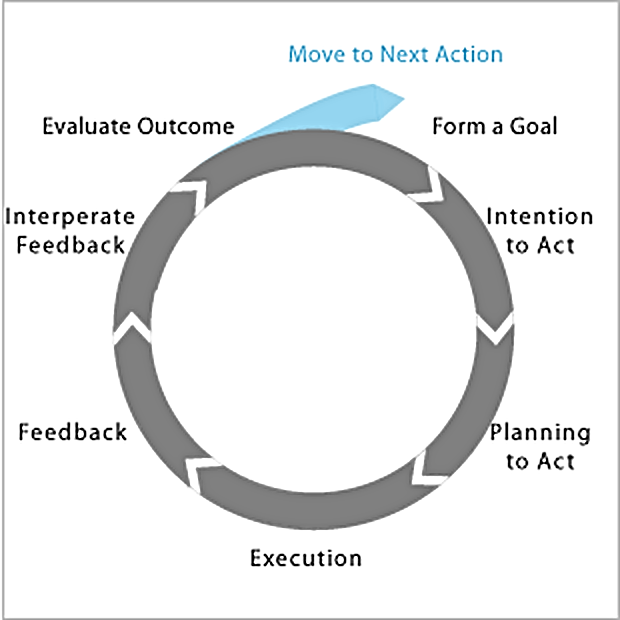
\includegraphics[width=0.4\textwidth]{grafiken/action_cycle.png}
 \caption{Human Action Cycle \cite{Kinser2011}}
 \label{fig:actionCycle}
\end{figure}
Um diesen Interaktionsverlauf zu gewährleisten und die Probleme zu minimieren, definierte Norman 6 Designprinzipien:
\begin{itemize}
	\item \textbf{Sichtbarkeit:} Wichtige Funktionen sollten für den Nutzer auf Anhieb sichtbar sein
	\item \textbf{Feedback:} Das System sollte nach einer Aktion sofort eine Rückmeldung geben
	\item \textbf{Einschränkungen:} Im aktuellen Zustand unzulässige Funktionen sollten ausgeblendet oder eindeutig erkennbar deaktiviert werden
	\item \textbf{Aktion und Wirkung:} Für jedes Interaktionselement sollte klar erkennbar sein, wie und worauf es sich auswirkt
	\item \textbf{Konsistenz:} Für identische Interaktionen sollten immer die gleichen Bedienelemente verwendet werden
	\item \textbf{Affordance:} Objekte sollten durch ihre Gestalt (Form, Farbe, etc.) eine Selbsterklärungsfähigkeit besitzen \cite{Ullenboom2014}
\end{itemize}
%%\subsubsection{Eingabegeräte} \label{sec:inputDevices}
%\heading{Maus}
%
%\heading{Tastatur}
%
%\heading{Touch}
\section{Visual Design} \label{sec:uid}
\textit{\enquote{Das Visual Design beschäftigt sich mit der Gestaltung einer Benutzeroberfläche \cite[S. 182]{Ullenboom2014}.}} Es baut auf den Beschlüssen in der Phase des Interaktionsdesign auf und verleiht der Oberfläche ihre finale Gestalt.\par
Der Visual Designer kümmert sich dabei um die Erstellung von prototypischen Designvorschlägen, die unter Anwendung von Designgrundlagen und -richtlinien entstehen. Das Ziel hierbei ist es, ein Konzept zu erstellen, das zugleich den Nutzer anspricht und zusätzlich die Usability durch Beachtung oben genannter Grundsätze verbessert. Im Laufe des Prozesses werden Objekte so platziert und gestaltet, dass eine einfache Orientierung möglich ist. Durch Farbkonzepte, basierend auf Erkenntnissen der Farbpsychologie, kann die Aufmerksamkeit konkret auf bestimmte Elemente gelenkt und Emotionen ausgelöst werden (durch Assoziation von Farben mit Elementen der Realität). Weitere Themengebiete sind Typographie, also das Auswählen von Schriftform, -größe, etc. und das Erstellen von Grafiken, Symbolen und Piktogrammen. \cite[S. 182]{Ullenboom2014}.

\subsection{Gestaltgesetze} \label{sec:uidRules}
Bei den Gestaltgesetzen handelt es sich um neuropsychologische Grundsätze, nach denen Objekte vom Menschen wahrgenommen und interpretiert werden. Berücksichtigt man diese Gesetze beim Design von Benutzeroberflächen, lassen sich Wahrnehmungseffekte auf subtile Weise erzeugen. Zum Beispiel kann die Aufmerksamkeit des Nutzers verstärkt auf gewisse UI-Elemente gelenkt oder die Bedienung vereinfacht werden. Nichtbeachtung dieser Regeln kann zu einer chaotisch wirkenden Benutzeroberfläche führen. Die wichtigsten Gestaltgesetze sind folgend aufgeführt.\par
\heading{Gesetz der Nähe}
\textit{\enquote{Objekte, welche nahe beieinander liegen, werden vom Auge gruppiert \cite[S. 186]{Moser2012}.}}\par
\begin{figure}[H]
 \centering
 
\includegraphics[width=0.25\textwidth]{grafiken/Gesetz_Naehe.png}
 \caption{Gesetz der Nähe \cite{Schossmann}}
 \label{fig:gesetzNaehe}
\end{figure} 
Durch Verringern der Abstände oder Vergrößern der Weißräume zwischen UI-Elementen, kann bewusst eine Gruppierung eingeführt werden, ohne dass zusätzliche Trennlinien oder Container von Nöten sind \cite[S. 186]{Moser2012}.\par
\heading{Gesetz der Ähnlichkeit}
\textit{\enquote{Visuell ähnliche Objekte werden vom Auge gruppiert \cite[S. 187]{Moser2012}.}}\par
\begin{figure}[H]
 \centering
 
\includegraphics[width=0.25\textwidth]{grafiken/Gesetz_Aehnl.png}
 \caption{Gesetz der Ähnlichkeit \cite{Grigo}}
 \label{fig:gesetzAehnl}
\end{figure} 
Schaltflächen können auch durch Verwendung verschiedener Formen, Farben oder Größen voneinander abgegrenzt und gruppiert werden. Besonders bei der Visualisierung von Datenbeständen in Diagrammen (Farbe und Form der Datenpunkte und der Legende) ist diese Eigenschaft hilfreich \cite[S. 187]{Moser2012}.\par
\heading{Gesetz der Prägnanz}
\textit{\enquote{In einer Vielzahl von Objekten werden diejenigen zuerst wahrgenommen, welche sich durch ein oder mehrere Merkmale vom Rest abheben \cite[S. 187]{Moser2012}.}}\par
\begin{figure}[H]
 \centering
 
\includegraphics[width=0.25\textwidth]{grafiken/praegnanz.png}
 \caption{Gesetz der Prägnanz}
 \label{fig:gesetzPraeg}
\end{figure}
Ist ein Element oder eine Information \enquote{besonders} dargestellt, wird sie als erstes wahrgenommen. So können wichtige Informationen oder Bedienelemente hervorgehoben werden.\par
\heading{Gesetz der Kontinuität}
\textit{\enquote{Dieses Gesetz besagt, dass zum Beispiel Linien an Schnittpunkten eher als Fortführung ihrer bisherigen Linienführung, denn als eine Richtungsänderung gesehen werden \cite{Grigo}.}}\par
\begin{figure}[H]
 \centering
 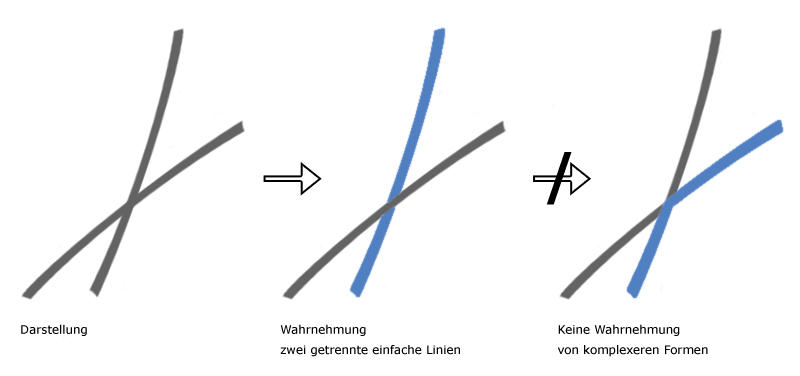
\includegraphics[width=0.8\textwidth]{grafiken/kontinuitaet.png}
 \caption{Gesetz der Kontinuität \cite{Grigo}}
 \label{fig:gesetzKonti}
\end{figure}
Elemente mit sanften Konturübergängen werden eher als Einheit erkannt als Elemente mit harten Übergängen \cite{Moser2012}.  Dies lässt sich unter anderem auf die Textorientierung anwenden. Sind mehrere Textzeilen nacheinander links orientiert, werden sie als zusammengehörig empfunden. Folgen daraufhin rechtsbündige Zeilen, bilden diese eine eigene Gruppe.\par
\heading{Gesetz der Geschlossenheit}
\textit{\enquote{Unser Auge komplettiert fehlende Teile einer Figur automatisch. \cite[S. 187]{Moser2012}.}}\par
\begin{figure}[H]
 \centering
 
\includegraphics[width=0.25\textwidth]{grafiken/geschlossenheit.png}
 \caption{Gesetz der Geschlossenheit \cite{WikiGestaltgesetze}}
 \label{fig:gesetzGeschloss}
\end{figure}
Das Gesetz der Geschlossenheit kann dazu dienen, die Komplexität von Bedienelementen zu reduzieren, indem Teile davon weggelassen werden. Die fehlenden Bereiche werden durch die Wahrnehmung automatisch ergänzt. Dieser Effekt funktioniert jedoch nur bei dem Nutzer bekannten Formen \cite{Moser2012}.\par
\heading{Gesetz des gemeinsamen Schicksals}
\textit{\enquote{Wenn sich mehrere Objekte gleichzeitig oder in die gleiche Richtung bewegen, so werden sie als zusammengehörig empfunden \cite[S. 187]{Moser2012}.}}\par
\begin{figure}[H]
 \centering
 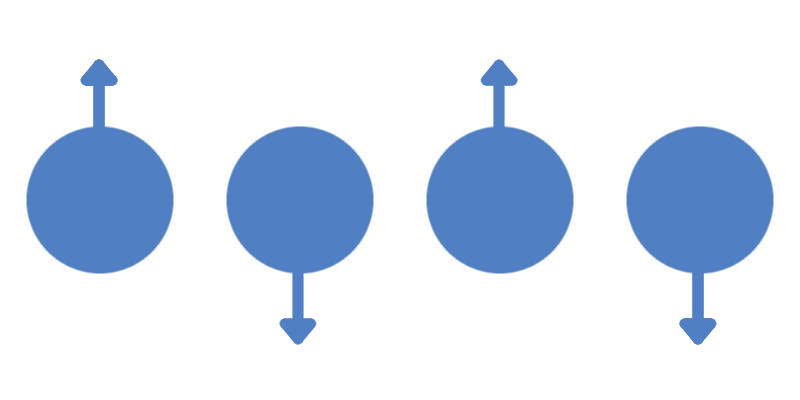
\includegraphics[width=0.2999\textwidth]{grafiken/schicksal.png}
 \caption{Gesetz des gemeinsamen Schicksals}
 \label{fig:gesetzSchicksal}
\end{figure}
Durch gleichzeitige bzw. gleichgerichtete Animation kann die Zusammengehörigkeit von Objekten erklärt werden \cite{Moser2012}. Unterschiedliche Animationen zur gleichen Zeit können dazu genutzt werden, die Unabhängigkeit verschiedener Gruppen zu betonen. In Abbildung \ref{fig:gesetzSchicksal} bspw. werden die sich nach oben und die sich nach unten bewegenden Elemente jeweils als eine Gruppe wahrgenommen.
\heading{Gesetz der gemeinsamen Region}
\textit{\enquote{Elemente in abgegrenzten Gebieten werden als zusammengehörig empfunden \cite{WikiGestaltgesetze}.}}\par
\begin{figure}[H]
 \centering
 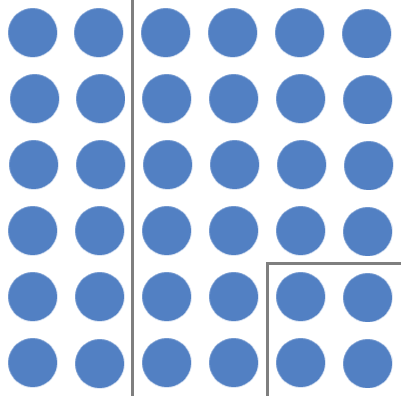
\includegraphics[width=0.25\textwidth]{grafiken/region.png}
 \caption{Gesetz der gemeinsamen Region}
 \label{fig:gesetzRegion}
\end{figure}
Die wohl trivialste Abgrenzung von Elementen kann durch die Benutzung von klassischen Trennlinien erfolgen. So werden die Objekte in mehrere Bereiche eingeteilt und innerhalb dieser Bereiche als zusammengehörig empfunden. Auch verschiedene Hintergrundfarben von Regionen führen zum gewünschten Effekt.

\subsection{DIN EN ISO 9241-110} \label{sec:uidNorms}
Sowohl im deutschen als auch internationalen Raum, gibt es seit geraumer Zeit Normen, die Grundsätze dafür liefern, wie Anwendungen gestaltet sein sollten. Für die Mensch-Computer-Interaktion ist insbesondere die \textit{DIN EN ISO 9241} von Bedeutung. In dieser sind Anforderungen an die Gestaltung von Hardware und Software, sowie das Arbeitsumfeld definiert. Besonders wichtig für das Thema User-Experience ist der Abschnitt 110. Dieser Abschnitt mit dem Titel \textit{Grundsätze der Dialoggestaltung} \enquote{behandelt die ergonomische Gestaltung von interaktiven Systemen und beschreibt Grundsätze der Dialoggestaltung, die grundsätzlich unabhängig von einer bestimmten Dialogtechnik sind, und die bei der Analyse, Gestaltung und Bewertung von interaktiven Systemen angewendet werden sollten \cite[S. 4]{DIN2006}.} Er wurde 2006 verfasst und ersetzt seitdem den vorherigen Teil 10 \cite{DIN2006}.\par
Um häufig auftretende Nutzungsprobleme zu vermeiden, definiert die Norm sieben Kriterien, nach denen die Gebrauchstauglichkeit einer Anwendung bewertet werden kann:
\begin{itemize}
	\item Aufgabenangemessenheit
	\item Selbstbeschreibungsfähigkeit
	\item Erwartungskonformität
	\item Lernförderlichkeit
	\item Steuerbarkeit
	\item Fehlertoleranz
	\item Individualisierbarkeit \cite[S. 7]{DIN2006}
\end{itemize}
Diese Kriterien überschneiden sich in einigen Punkten mit den von Nielsen definierten Kernaspekten der Usability, führen aber ergänzend die Selbstbeschreibungsfähigkeit, Steuerbarkeit und Individualisierbarkeit an.\par
Ein Dialog ist selbstbeschreibungsfähig, wenn ein Nutzer zu jeder Zeit feststellen kann, an welcher Stelle im Dialog er sich befindet, weiß, wie und wohin er von dort navigieren kann und welche Aktionen in der aktuellen Ansicht möglich sind \cite[S. 10]{DIN2006}. Die Steuerbarkeit beschreibt die Adaptivität des Dialogs an die Fähigkeiten und das Navigationsverhalten des Anwenders. Die Geschwindigkeit in der ein Nutzer Aktionen auf der Oberfläche durchführt, sollte möglichst allein durch den Nutzer bestimmt werden. Weiterhin sollte die Navigation den Nutzer nicht einschränken, sondern ihre Möglichkeiten aufzeigen und eine freie Navigation unterstützen \cite[S.13]{DIN2006}. Ein individualisierbarer Dialog ermöglicht es, die Informationsdarstellung in einem gewissen Rahmen an die Bedürfnisse des Anwenders anzupassen \cite[S.15]{DIN2006}. \par
Es ist nicht immer möglich, alle Grundsätze zu erfüllen. Stattdessen muss von Anwendung zu Anwendung gewichtet werden, auf welchen Aspekten der Schwerpunkt liegt. Beschränkende Faktoren können auf der einen Seite Budget- oder Zeitmangel sein, auf der anderen Seite können sich die Kriterien aber auch gegenseitig einschränken. Beispielsweise ist es schwerer möglich, eine gute Steuerbarkeit zu erreichen, wenn die Applikation hochindividualisierbar sein soll \cite{DIN2006}. Daher muss für eine gute Usability abgewägt werden, worauf bei der Umsetzung der Fokus gelegt werden soll.

\section{Usability-Evaluationsverfahren} \label{sec:methods}
Es gibt verschiedene Verfahrensweisen, die mit unterschiedlich viel Aufwand Aufschluss über die Gebrauchstauglichkeit einer Anwendung geben können. \enquote{Sie alle versuchen, durch unterschiedliche Ansätze, eine Aussage darüber zu treffen, wie effizient, effektiv und zufriedenstellend das Produkt von einem Benutzer verwendet werden kann. Jede Methode hat ihre eigenen Vor- und Nachteile \cite[S. 224]{Ullenboom2014}.}\par
Die Evaluationsmethoden können in zwei Arten unterteilt werden. Zum einen gibt es die analytischen Nutzertests, für die eine Gruppe an Testpersonen ausgewählt wird, die daraufhin Fragen beantworten oder Aufgaben mit dem Testsystem durchführen müssen. Die andere Art von Tests sind die die empirischen Expertentests. Für diese Analysen werden keine Testpersonen benötigt. Stattdessen wird anhand objektiver Kriterien und Verfahren versucht, die Effektivität, Effizienz und Nutzerzufriedenheit zu erhöhen. Für die Auswahl der zu verwenden Testmethoden müssen sowohl die Anforderungen an diese, als auch die Güte der Methoden in Betracht gezogen werden. Je nach Art des Testes stellt dieser Ansprüche an das Fachwissen des Testers und den nötigen Aufwand um die Tests durchzuführen. Der Nutzen eines Tests setzt sich aus seiner Objektvität, seiner Zuverlässigkeit und seiner Gültigkeit zusammen \cite[S.224 f.]{Ullenboom2014}.\par
Der Ablauf eines gesamten Testvorganges ist nach Ullenboom folgender:
\begin{enumerate}
	\item \textbf{Ziel und Zweck festlegen:} Es muss festgelegt werden, was der Untersuchungsgegenstand ist und was der Zweck der Untersuchung ist
	\item \textbf{Untersuchungsdesign entwerfen:} Bei dem Entwurf müssen Faktoren wie Zeit, Ressourcen und Stand des Projektes mit einbezogen werden
	\item \textbf{Teilnehmer rekrutieren:} Bei Nutzertests müssen Teilnehmer ausgewählt werden, die nach Möglichkeit verschiedene Anwendertypen repräsentieren.
	\item \textbf{Evaluation vorbereiten:} Das Szenario, das getestet werden soll, muss vorbereitet und die entsprechende Testumgebung geschaffen werden.
	\item \textbf{Evaluation durchführen} Die Tests werden durchgeführt. Währenddessen wird das Verhalten der Nutzer dokumentiert. Dies beinhaltet unter Anderem, wie zielgerichtet der Anwender die gegebenen Aufgaben lösen kann.
	\item \textbf{Resultate auswerten:} Anhand der dokumentierten Daten können nun Problemstellen identifiziert und ausgebessert werden. Dazu erfolgt im Team eine Gewichtung der Probleme und wenn möglich die Aufnahme erster Lösungsansätze.
\end{enumerate}
Für die Durchführung der Nutzertests ist nach Nielsen eine Probandengruppe von 5 Personen völlig ausreichend. Studien zufolge entdeckt ein einzelner Testanwender rund 31\% der Usability-Probleme einer Anwendung \cite{Nielsen2000}. Testet man mit mehreren Nutzern, findet jeder dieser Nutzer im Mittel 31\% der vorhandenen Fehler. Dabei werden zum Teil neue Probleme ans Licht gebracht, aber auch bereits bekannte wiederholt entdeckt. Forschungen haben ergeben, dass der Anteil gefundener Usability-Probleme aus diesem Grund wie folgt berechnet werden kann:
\begin{equation}
			1-(1-L)^n\text{ \cite{Nielsen2000}}
\end{equation}
Dabei ist \(n\) die Anzahl an Testpersonen und \(L\) der Anteil gefundener Usability-Probleme pro Testsubjekt (31\%) \cite{Nielsen2000}. Das bedeutet bei 5 Testpersonen eine Abdeckung von rund 85\%. Das Testen mit mehr Anwendern würde das Budget stark belasten und wenig zusätzlichen Nutzen mit sich bringen. Daher ist es sinnvoller, in vielen Durchläufen mit wenigen Personen zu testen, als in wenigen Durchläufen mit vielen \cite{Nielsen2000}.\par
\heading{Hallway-Testing}
Das Hallway-Testing ist eine sehr informelle Methode, erstes Feedback über die Usability eines kleinen Programmteiles zu erhalten. Das Prinzip des Hallway-Testing ist es, einen beliebigen zu fragen, was er von einer bestimmten Funktion hält. Dazu wird eine kurze Aufgabe gestellt (wie z.B. \enquote{Drucke dieses Dokument}) und beobachtet, wie der Kandidat sich verhält. Bei komplexeren Sachverhalten wird so kurz wie möglich die Fachlichkeit bzw. der Nutzungskontext erklärt. Ohne Hinweise für die Lösung zu geben, wird die Aufgabe kurz erklärt. Bei der Durchführung denkt der Testnutzer laut mit \cite[S. 226]{Ullenboom2014}.
Mit sehr wenig Aufwand können durch diese Methode während der Entwicklung grobe Nutzungsprobleme beseitigt werden.\par
\heading{Pluralistic Walkthrough}
Beim Pluralistic Walkthrough handelt e sich um eine Art von Nutzertests. Die Testkandidaten werden in einer Art Workshop versammelt und bekommen die Anwendung grob vorgestellst, sodass sie sich auf dem Wissensstand eines durchschnittlichen Erstbenutzers befinden. Daraufhin wird die Aufgabenstellung unterbreitet und die Nutzer versuchen diese mit der ihnen gegebenen Anwendung umzusetzen. Am Ende des Tests wird die Optimallösung vorgestellt. Die Testanwender beschreiben daraufhin ihre Lösung. Zum Feststellen der konkreten Usability-Probleme, also der Gründe, warum eine andere Lösung gewählt oder gefunden wurde, wird zum Abschluss über die Lösungen diskutiert und die Fehlerquellen herausgearbeitet \cite[S. 228]{Ullenboom2014}.\par
\heading{Formaler Usability-Test}
Bei dieser Methode werden Testpersonen einzeln mit der Bedienung eines Programmes betraut. Nachdem festgelegt wurde, welche Teile der Anwendung getestet werden sollen, werden Aufgaben formuliert und niedergeschrieben. Diese Aufgaben erhält der Testkandidat in schriftlicher Form. Er versucht diese mit der vorliegenden Anwendung zu lösen und wird währenddessen beobachtet. Zu diesem Zweck wird zum Einen der Bildschirminhalt aufgezeichnet und zum anderen die Reaktion des Teilnehmers selbst analysiert \cite[S. 230]{Ullenboom2014}.\par
Der Test muss sorgsam vorbereitet werden. Dazu gehört sowohl die Installation der zu testenden Software, als auch das Aufsetzen des Aufnahmemoduls, dass die Interaktion und ggf. den Nutzer selbst aufzeichnet. Um die Aufgabenstellungen lösen zu können, sind ggf. Testdaten erforderlich, die erst noch eingespielt werden müssen. Auch darf nicht vergessen werden, das System zurückzusetzen, nachdem ein Testnutzer Änderungen daran gemacht hat. \cite[S.231]{Ullenboom2014}\par
Während der Instruktion des Nutzers wird dieser gebeten, während des Tests laut mitzudenken. Diese Technik wird \textbf{\textit{Thinking Aloud}} genannt. Dies hilft dabei, die Absichten, Gefühle und Eindrücke des Anwenders zu ergründen \cite[S. 1]{Fromman2005}. Nach Start des Tests wird durch das Testpersonal keine Hilfestellung mehr gegeben. Weiß der Nutzer nicht, wie er weiter zu verfahren hat, wird der Testdurchlauf abgebrochen \cite[S. 231]{Ullenboom2014}.
\heading{Heuristische Evaluation}
Die Heuristische Evaluation ist ein beliebtes Expertentestverfahren. Der Tester untersucht im Rahmen dieser Methode eine Anwendung auf Basis von Heuristiken. In der Regel werden mehrere Usability-Experten eingesetzt, um die Erkennungsrate von Problemen zu erhöhen. Am Ende werden die Ergebnisse zusammengetragen und für jedes gefundene Problem ein Schweregrad ermittelt. Dieser setzt sich aus den Faktoren \textit{Auftretenswahrschienlichkeit}, \textit{Grad der Beeinflussung} und \textit{der Möglichkeit, das Problem zu umgehen}, zusammen. Da die definierten Heuristiken eine gewisse Sicherheit bieten, kann diese Methode auch von weniger erfahrenen Testern angewandt werden \cite[S. 232f.]{Ullenboom2014}.\par
\heading{Cognitive Walkthrough}
Der Expertentest \enquote{Cognitive Walkthrough} ist ein Verfahren, bei dem der Usability-Tester versucht, sich in die Lage des Anwenders zu versetzen und die Anwendung zu bedienen. Um dies adäquat tun zu können, müssen zunächst die genauen Arbeitsabläufe der Endanwender erschlossen werden. Hierbei ist es sinnvoll, verstärkt komplexe Arbeitsabläufe zu testen \cite[S. 234]{Ullenboom2014}.\par
Der erste Schritt der Analyse ist die \textit{Definition des Inputs}. Nach Ullenboom sind dazu folgende Schritte notwendig:
\begin{enumerate}
	\item Festlegen, welcher Teil getestet werden soll
	\item Verstehen der Arbeitsabläufe
	\item Formulieren von praxisnahen Aufgaben
	\item Wahl einer geeigneten Benutzerrolle
	\item Vorbereiten eines Prototypen \cite[S. 234]{Ullenboom2014}
\end{enumerate}
Bei der Durchführung werden die Aufgaben anhand des Prototypens versucht umzusetzen. Dabei wird davon ausgegangen, dass der Nutzer stets versucht, den Weg zu nehmen, den er für den einfachsten hält. Es muss bei jeder Aktion geprüft werden, ob während der Interaktion die folgenden Fragen geklärt werden:
\begin{itemize}
	\item Wird der Benutzer versuchen, den richtigen Effekt zu erzielen?
	\item Wird der Benutzer erkennen, dass die korrekte Aktion zur Verfügung steht?
	\item Wird der Benutzer eine Verbindung zwischen der korrekten Aktion und dem gewünschten Effekt herstellen?
	\item Wenn die korrekte Aktion ausgeführt wurde: Wird der Benutzer den Fortschritt erkennen? \cite[S. 234]{Ullenboom2014}
\end{itemize}
Wenn sich bei einer dieser Fragestellungen Probleme zeigen, müssen diese unter Angabe des entsprechenden Handlungsschrittes, dem Grund der Probleme und möglicher Verbesserungsvorschläge dokumentiert werden. Aufgrund dieser Aufzeichnungen kann die Benutzerschnittstelle überarbeitet werden.\par
\heading{Usability-Befragung}
\enquote{Die Usability-Befragung ist eine quantitative Methode, bei der die Usability mit Hilfe eines Fragebogens ermittelt wird \cite[S. 236]{Ullenboom2014}.} Es ist eine Art von Nutzertest, die darauf abzielt, einen möglichst großen Anwenderbereich abzudecken. Für die Auswahl des Fragebogens gibt es mehrere Möglichkeiten:
\begin{enumerate}
	\item \textbf{Standardisierter Fragebogen:} Es gibt eine Reihe standardisierter Fragebögen, mit deren Hilfe ein Grobüberblick über verschiedene Aspekte der Usability einer Anwendung erlangt werden kann.
	\item \textbf{Teilstandardisierter Fragebogen:} Verwendung von standardisierten Fragebögen, angepasst an die zu evaluierende Anwendung (z.B. Freitextfelder für weitergehende Informationen)
	\item Selbstentwickelter Fragebogen: Durch die Entwicklung eines speziell auf die Anwendung zugeschnittenen Fragebogens können die exaktesten Ergebnisse erzielt und konkrete Problemstellen identifiziert werden. Dies erfordert allerdings einigen Aufwand und entsprechendes Know-How.
\end{enumerate}
\heading{KLM/GOMS}
\textit{GOMS} ist eine Methode zur Evaluation der Effizienz eines Softwaresystems. Durch das Anwenden gewisser Regeln ist es möglich, die Zeitdauer abzuschätzen, die für eine Interaktion benötigt wird. Dazu ist es zuerst von Nöten, alle Schritte der Interaktion zu identifizieren. Diese Schritte werden in atomare Aktivitäten zerlegt, deren einzelne durchschnittliche Dauer durch empirische Analysen ermittelt wurde.\par
GOMS steht für \textit{Goals, Operators, Methods and Selection Rules}. Dies ist gleichzeitig das Modell, das der Interaktion eines Benutzers zugrunde liegt:
\begin{itemize}
	\item \textbf{Ziele:} Die Ziele, die der Benutzer erreichen möchte (Bsp. Dokument drucken)
	\item \textbf{Operatoren:} Die atomaren Handlungsschritte (Bsp. Drücken einer Taste, Warten auf Feedback der Software)
	\item \textbf{Methoden:} Kombination von Operatoren zu einer Interaktion, die den Nutzer an sein Ziel bringt
	\item \textbf{Selektionsregeln:} Nach diesen Regeln entscheidet der Benutzer, welche mögliche Methode er einsetzt
\end{itemize}
KLM-GOMS ist eine spezielle, einfache Variante des GOMS-Modells. Es verwendet nur sechs Operatoren, die die atomaren Handlungsschritte darstellen:
\begin{table}[h!]
 \centering
 \begin{tabular}{|l|c|r|} \hline
 \textbf{Aktion} & \textbf{Code} & \textbf{Dauer} \\ \hline
 Tastendruck & K & \specialcell{Profi Schreiber:&\myTab 0.08 s\\Guter Schreiber:&\myTab 0.20 s\\Anfänger:&\myTab 1.20 s\\Zufällige Buchst.:&\myTab 0.50 s\\Codes:&\myTab 0.75 s} \\ \hline
 Maus positionieren & P & 1.1 s \\ \hline
 Tastatur-/Maus- Wechsel & H & 0.4 s \\ \hline
 Maustaste & B & 0.1 s \\ \hline
 Kurz überlegen & M & 1.2 s \\ \hline
 Antwortzeit & W(t) & Unterschiedlich (je nach t) \\ \hline
 \end{tabular}
 \caption{KLM Zeitwerttabelle}
 \label{tab:klm}
\end{table}
\heading{A/B-Test}
A/B-Tests dienen dazu, zwei verschiedene Produkte oder Lösungsvarianten miteinander zu vergleichen. Dies geschieht in der Regel in Form von Nutzertests. Dabei bedienen zwei Nutzergruppen gleichzeitig die verschiedenen Systeme und versuchen eine gestellte Aufgabe zu lösen. Dazu wird ein Kriterium definiert, anhand dessen bestimmt werden kann, ob die Interaktion erfolgreich war (z.B. Operationen so gewählt wie durch das Design vorgesehen). Die Lösung, bei der die Testnutzer quantitativ erfolgreicher waren, ist die Alternative mit der besseren Usability \cite[S. 240]{Ullenboom2014}.\par
Zum Vergleich der Effizienz zweier Anwendung wird häufig eine GOMS-Analyse der beiden Software-Produkte durchgeführt. Dies muss mit vergleichbaren Aufgabenstellungen geschehen, damit die Ergebnisse repräsentativ sind.\par
\heading{Eyetracking}
Eytracking ist eine ergänzende Methode, die die Aussagefähigkeit eines Nutzertests erhöhen kann. Es zielt speziell darauf ab, zu erkennen, welchen Bereichen der Anwender vermehrt Aufmerksamkeit schenkt und welche er gar nicht beachtet \cite{Henrici2010}.\par
Es gibt verschiedene technische Lösungen, um Eyetracking umzusetzen. Eine davon ist die Benutzung einer Eyetracking-Kamera, die zusätzlich zu einem Monitor aufgestellt werden kann. Das Modul besteht aus einer Kameralinse und einer Infrarot-Lichtquelle. Das für das menschliche Auge unsichtbare Infrarot-Licht erzeugt auf der Hornhaut eine sogenannte \enquote{korneale Reflexion}. Diese Reflexion befindet sich immer über, unter oder neben der Pupille. die Pupille selbst reflektiert das Licht nicht. Aus der relativen Position der Reflexion zur Pupille kann nach geeigneter Kalibrierung der Blickpunkt auf dem Bildschirm errechnet werden.\par
\begin{figure}[H]
 \centering
 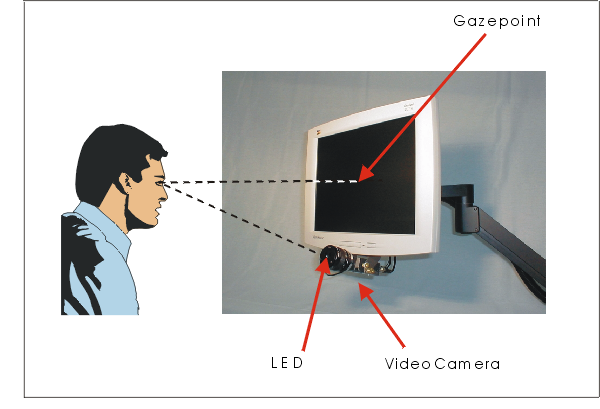
\includegraphics[width=0.45\textwidth]{grafiken/eyegaze.png}
 \caption{Eyetracking \cite{Eyegaze}}
 \label{fig:eyetracking}
\end{figure}
Während der Aufzeichnung können typischerweise zwei wesentliche Arten von Daten gesammelt werden, die mit der Blickrichtung zusammen hängen. Dies sind die Fixation und die Sakkade. Unter Fixation wird der Fokussierung der Augen auf einen bestimmten Bildpunkt verstanden. Dazu gehört die Position und die Dauer der Fokussierung. Eine Sakkade ist der Sprung von einer Fixation zur nächsten. Dies geschieht extrem schnell, sodass zu dieser Zeit mit herkömmlichen Eyetracking-Systemen keine verwertbaren Daten gemessen werden können. Zusätzlich zu diesen Informationen lässt sich auch die Pupillengröße ermitteln. Diese Daten sind allerdings im Rahmen der Usability-Tests kaum von Relevanz.\par
Die gesammelten Daten lassen sich nun auf mehrere Arten und Weisen visualisieren \cite{Henrici2010}.\par
Heatmaps und Gaze-Opacity Visualisierungen  zeigen mithilfe von Farbcodes, auf welchen Elementen bzw. Bereichen Fixationen erkannt wurden und wie lange diese gedauert haben. Dabei stehen warme Farben meist für längere Fixationen. Parallel dazu lässt sich eine Gaze Opacity Grafik erstellen, die Bereiche schwarz einfärbt, wenn diese kaum oder gar nicht wahrgenommen wurden \cite{Henrici2010}.
\begin{figure}[H]
 \centering
 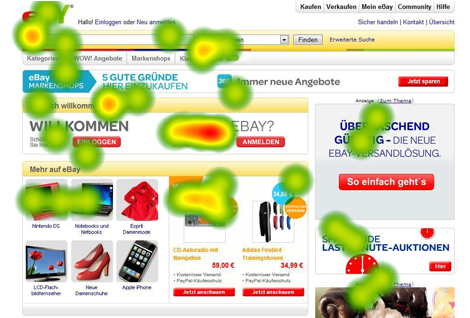
\includegraphics[width=0.48\textwidth]{grafiken/heatmap.png}
 \caption{Beispiel Heatmap \cite{Henrici2010}}
 \label{fig:heatmap}
\end{figure}
\begin{figure}[H]
 \centering
 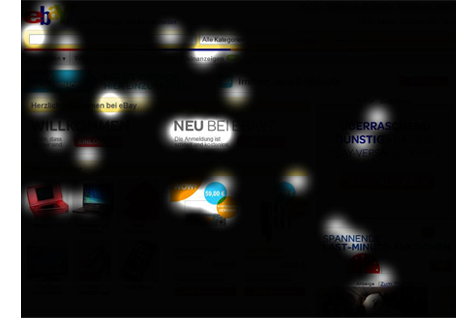
\includegraphics[width=0.48\textwidth]{grafiken/gaze_opacity.png}
 \caption{Beispiel Gaze Opacity \cite{Henrici2010}}
 \label{fig:gazeOpacity}
\end{figure}
Bei der Areas of Interest wird die Oberfläche in verschiedene Bereiche eingeteilt. Die Fixationen in den einzelnen Bereichen werden zusammengezählt und der prozentuale Anteil hinsichtlich der Gesamtheit der Fixationen (und ihrer Dauer) während des gesamten Tests ermittelt. Jedem Bereich kann eine Farbe zugewiesen werden, die als Schlüssel zu der in der Legende festgehaltenen Prozentzahl dient.
\begin{figure}[H]
 \centering
 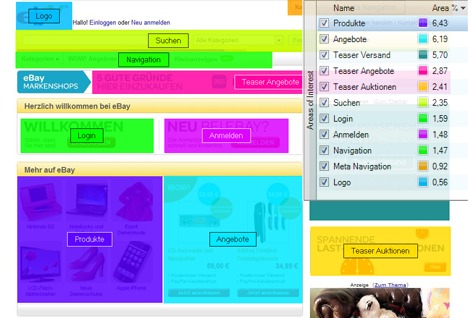
\includegraphics[width=0.48\textwidth]{grafiken/areas_of_interest.png}
 \caption{Beispiel Areas of Interest \cite{Henrici2010}}
 \label{fig:areasOfInterest}
\end{figure}
Die letzte Visualisierung beachtet zusätzlich die Reihenfolge der Fixationen. Es werden verschieden große Kreise genutzt, um Fixationen unterschiedlicher Dauer darzustellen. Diese werden in der richtigen Reihenfolge durch Linien verbunden, welche die synthetisierten Sakkaden darstellen.
\begin{figure}[H]
 \centering
 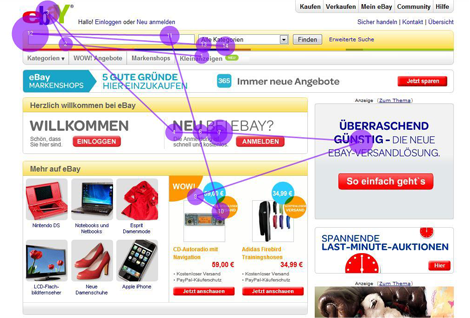
\includegraphics[width=0.48\textwidth]{grafiken/gaze_plot.png}
 \caption{Beispiel Gaze Plot \cite{Henrici2010}}
 \label{fig:gazePlot}
\end{figure}
\heading{Bewertung der Testverfahren}
Die Testverfahren können nach verschiedenen Kriterien bewertet werden. Ein Teil der Kriterien betrachtet die Anforderungen an das Budget und den Tester, der andere Teil beschäftigt sich mit der Qualität der Ergebnisse. Optimal sind Tests, wenn sie möglichst geringe Anforderungen haben, aber aussagekräftige Ergebnisse liefern. Ein Faktor, der in dieser Übersicht nicht bedacht ist, ist der Zeitpunkt, zu dem die Tests durchgeführt werden können. Das Hallway Testing kann bspw. nur während einer laufenden Entwicklung an einer Komponente durchgeführt werden und eignet sich nicht als Testmethode für ein, möglicherweise komplexes, fertiges System.
\begin{table}[h!]
		\begin{tabular}{|l|c|c|c|c|c|c|}
			\hline
			\textbf{Methode}&\textbf{Fachwis.}&\textbf{Aufwand}&\textbf{Effektiv.}&\textbf{Validität}&\textbf{Zuverl.}&\textbf{Objektiv.}\\
			\hline
			\twolinecell{Hallway\\Testing} & \star & \star & \star \star & \star & \star & \star\\
			\hline
			\twolinecell{Usability\\Walkthrough} & \star \star & \star \star & \star \star & \star \star & \star & \star\\
			\hline
			\twolinecell{Formaler\\Usability-Test} & \star \star & \star \star \star & \star \star \star & \star \star \star & \star \star & \star \star\\
			\hline								
			\twolinecell{A/B-Test\\[2.3ex]} & \star \star & \star \star & \star \star & \star \star \star & \star \star & \star \star \star\\
			\hline
			\twolinecell{Heuristische\\Evaluation} & \star \star \star & \star & \star \star \star & \star \star & \star \star \star & \star\\
			\hline
			\twolinecell{Usability-\\Befragung} & \star & \star & \star & \star \star & \star \star & \star \star \star\\
			\hline
			\twolinecell{GOMS\\[2.3ex]} & \star \star & \star \star & \star & \star \star & \star \star \star & \star \star \star\\
			\hline
		\end{tabular}
		\caption{Gütekriterien von Evaluationsmethoden nach Ullenboom \cite[S. 225]{Ullenboom2014}}
	\label{tab:hallwayTesting}
\end{table}
\section{JavaFX} \label{sec:javaFX}
JavaFX ist das aktuellste GUI-Framework der Java-Plattform. Es wird standardmäßig mit Java SE 8 ausgeliefert und soll den Vorgänger \textit{Swing} ersetzen \cite{Mueller2015}.\par
Die neuartige Technologie vereinigt verschiedene Konzepte, die den Entwickler bei der Entwicklung einer Benutzeroberfläche unterstützen.
\begin{itemize}
	\item \textbf{\textit{Szenegraph}:} Sämtliche Bedienelemente sind in einer Baumstruktur, ausgehend von einem Wurzelknoten, angeordnet.
	\item \textbf{Styling:} Das Aussehen aller UI-Komponenten kann mit Hilfe von CSS-Dateien angepasst werden.
	\item \textbf{Animationen:} Es können auf unkomplizierte Weise Animationen erstellt und auf beliebige angezeigte Objekte angewandt werden.
	\item \textbf{FXML:} Die Struktur der Oberfläche kann sowohl in Java-Code, als auch in XML-basierten Dateien, sogenannten FXML-Dateien, definiert werden.
	\item \textbf{Properties und Bindings:} Alle Controls haben gewisse Eigenschaften (Properties), die sich dynamisch verändern lassen. So kann man ein Property an ein gleichartiges binden. Verändert sich der Wert der einen Eigenschaft, wird der Wert der anderen ebenfalls geändert.
\end{itemize}
\subsection{Eventhandling} \label{sec:javafxEventhandling}
Besonders relevant für die Arbeit ist das Konzept des Eventhandlings in JavaFX.\par
Ein Event ist eine Eingabe, die durch den Nutzer getätigt wurde. Dies kann z.B. das Drücken oder Loslassen einer Taste auf der Tastatur sein. Auch das Klicken auf ein Bedienelement und das Ausführen einer Geste auf einem Touchscreen stellen Events dar. Jedes dieser Events kann an bestimmten Stellen im Code behandelt werden.\par
Wie in Abschnitt \ref{sec:javaFX} bereits erwähnt, ist die Komponentenstruktur in JavaFX baumartig aufgebaut. Der Wurzelknoten im Szenegraphen ist die \textit{Stage}. Diese entspricht dem sichtbaren Fenster, in dem die Anwendung läuft. Sie hat als einziges Kind die \textit{Scene}, die alle weiteren Elemente enthält.
\begin{figure}[H]
 \centering
 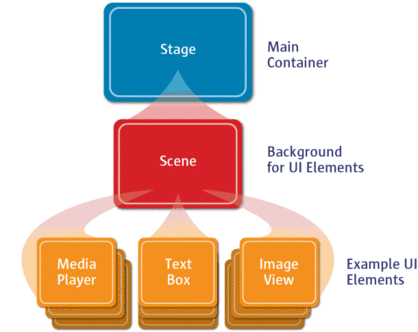
\includegraphics[width=0.45\textwidth]{grafiken/scenegraph.png}
 \caption{Aufbau Szenegraph \cite{Jakob2015}}
 \label{fig:scenegraph}
\end{figure} 
Zu den Knoten (in JavaFX \textit{Node}s gennant) gehören \textit{Branch Nodes} bzw. Container und \textit{Leaf Nodes}, also konkrete Bedienelemente. Die Container dienen dazu, die Bedienelemente oder weitere Container zu kapseln und diese auf eine eigene Art und Weise auf der Benutzeroberfläche anzuordnen. Dadurch ergibt sich die Baumstruktur des Szenegraphen:
\begin{figure}[H]
 \centering
 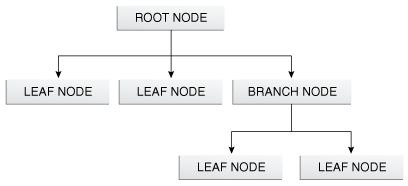
\includegraphics[width=0.45\textwidth]{grafiken/scenegraph2.png}
 \caption{Beispiel Szenegraph \cite{Hommel2013}}
 \label{fig:scenegraph2}
\end{figure} 
Jeder Standardknoten aus der JavaFX-Bibliothek implementiert ein Interface namens \textit{EventTarget}. Die Phasen, die ein Event durchläuft sind folgende:
\begin{enumerate}
	\item \textbf{Target selection:} Das Ziel des Events wird bestimmt (Bei Mausklick z.B. das Element, auf dem der Cursor ruht)
	\item \textbf{Route construction:} Die Route vom Wurzelknoten zum Ziel wird konstruiert
	\item \textbf{Event capturing:} Der Weg des Events vom Wurzelknoten zu dem Zielknoten
	\item \textbf{Event bubbling:} Der Weg des Events vom Zielknoten zurück zum Wurzelknoten
\end{enumerate}
Für das Eventhandling sind die Phasen \textit{Event Capturing} und \textit{Event Bubbling} die wichtigsten. Das Event \enquote{bewegt} sich auf der in Phase 2 konstruierten Route bis zum Zielknoten. Dabei passiert es zunächst den Wurzelknoten und weiterhin jeden Knoten, der im Baum des Szenegraphen zwischen diesem und dem Zielknoten liegt. Dies ist die \textit{Event Capturing} Phase. In der \textit{Event Bubbling} Phase nimmt das Event dann genau den umgekehrten Weg. Es bewegt sich vom Zielknoten zurück zum Wurzelknoten.\par
Das Event kann an jedem beliebigen Knoten bearbeitet werden, der auf dieser Route liegt. Soll ein Event in der \textit{Capturing}-Phase behandelt werden, muss ein Event-Filter an der entsprechenden Komponente registriert werden. Standardmäßig werden jedoch eher Event-Handler registriert, deren Code in der \textit{Bubbling}-Phase ausgeführt wird. Es ist durchaus möglich, einer Komponente mehrere Handler oder Filter hinzuzufügen, jedoch ist die Ausführungsreihenfolge innerhalb einer Phase nicht definiert. Zusätzlich gibt es \textit{Convenience}-Methoden, die das Hinzufügen eines \textit{Event-Handlers} vereinfachen, da der Typ des zu behandelnden Events nicht explizit angegeben werden muss. Zu beachten ist hierbei, dass die über die \textit{Convenience}-Methoden hinzugefügten Event-Handler pro Komponente erst nach den anderen Handlern ausgeführt werden und es nur genau einen pro Eventtyp gibt.\par
\begin{figure}[H]
 \centering
 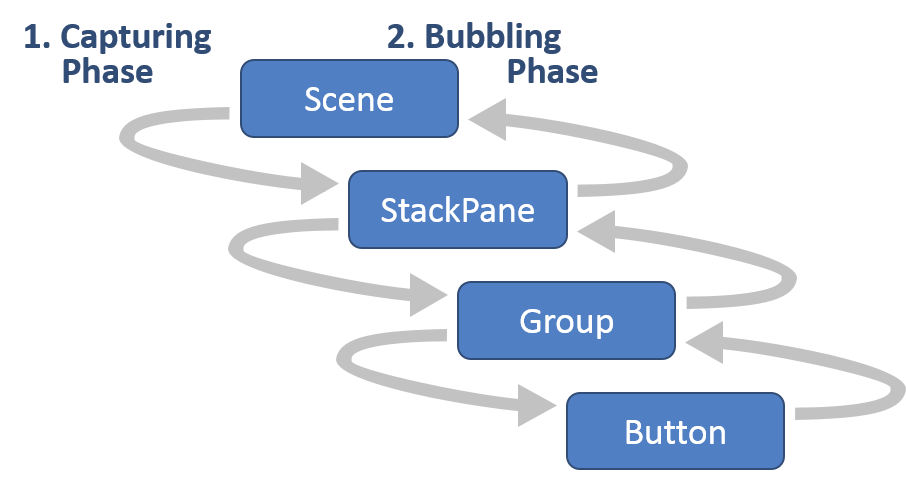
\includegraphics[width=0.75\textwidth]{grafiken/event_phase.png}
 \caption{Event Capturing und Bubbling}
 \label{fig:eventPhase}
\end{figure} 
Ist die Behandlung eines Events an einem bestimmten Knoten abgeschlossen, kann das Event entweder an den nächsten Knoten weitergereicht oder konsumiert werden. Wird das Event durch den Handler bzw. Filter konsumiert, wird es nicht weitergereicht und die Bearbeitung ist damit abgeschlossen.\par
\section{Die Anwendung \enquote{FalkoFX}} \label{sec:application}
Das Softwareprojekt \textit{Falko} beschäftigt sich mit der Visualisierung, Erstellung und Pflege länderspezifischer Fahrzeugdaten. Bei \textit{FalkoFX} handelt es sich um ein Unterprojekt für die Entwicklung eines weiteren Clients, der für einen Teil der Benutzer eine bessere Übersicht bietet und so eine höhere Produktivität ermöglicht. Das Projekt wird mit Java 8 und der JavaFX-Technologie umgesetzt.\par
Der FalkoFX-Client verfolgt, im Vergleich zu dem sehr umfangreichen Falko-Client, um einiges stärker den Ansatz der Usability. Neue Funktionalitäten werden zunächst fachlich durchgeplant und daraufhin mehrere Designkonzepte entworfen und vorgestellt. Moderne Bedienelemente, die von den Standardkomponenten zum Teil stark abweichen, wurden entworfen, um ein gutes, intuitives Nutzungsempfinden zu ermöglichen.\par
Das Software-System ist in verschiedene Anwendungsfälle untergliedert. Jeder Anwendungsfall hat ein eigenes zugrundeliegendes Datenmodell von Daten, die verglichen und aufbereitet angezeigt werden können. Wird über die Hauptnavigation in einen Anwendungsfall gewechselt, ist der erste Schritt das Auswählen der zu anzuzeigenden Daten. Dies geschieht über einen Filter, der anhand von Kriterien konfiguriert werden kann. Der nächste Schritt ist die Anzeige der Daten. In jedem Anwendungsfall stehen unterschiedliche Ergebnispräsentationen zur Verfügung, zwischen denen gewählt werden kann. Die verfügbaren Arten der Ergebnispräsentation begründen sich auf die Natur der unterliegenden Datenmodelle. Zu jedem in der Ergebnisansicht angezeigten Elemente können die Details aufgerufen werden.\par
\section{Responsive Design} %SubSection?
Das Responsive Design ist ein aus der Webentwicklung stammender Begriff. Es beschreibt die Fähigkeit einer Anwendung oder Webseite, auf verschiedenen Monitorgrößen darstellbar und benutzbar zu sein. So kann z.B. eine Webseite, die nach Richtlinien des Responsive Design erstellt wurde, sowohl auf einem Computermonitor (unabhängig von der Auflösung), als auch auf einem Tablet und einem Smartphone korrekt angezeigt werden.\par
\begin{figure}[H]
 \centering
 
\includegraphics[width=0.5\textwidth]{grafiken/responsive_design.png}
 \caption{Beispiellayout Responsive Design \cite{Moon2013}}
 \label{fig:responsiveDesign}
\end{figure} 
\chapter{Interaktionsdesign}
%In diesem Abschnitt soll analysiert werden, wie die möglichen Interaktionen gestaltet sind. %Werden die Designprinzipien Normans (Kap. \ref{sec:interactionDesign}) nicht hinreichend erfüllt, lässt dies auf ein zu behebendes Problem der User-Experience schließen.
Da es sich bei \textit{FalkoFX} um eine bestehende Anwendung in der Entwicklungsphase handelt, ist bereits ein implizites Interaktionskonzept gegeben. Dieses wird im Folgenden analysiert und erläutert, um eine Orientierung zu ermöglichen. Spezielle Designentscheidungen werden dabei hervorgehoben. Das Hauptaugenmerk dieses Abschnittes wird auf der Entwicklung alternativer Eingabemethoden liegen, die es dem Nutzer ermöglichen sollen, die vorhandenen Interaktionen intuitiver und mit dem Eingabegerät seiner Wahl durchführen zu können. Zudem wird die Anwendung auf eine Benutzung an Tablet-PCs und anderen Geräten mit Touch-Bedienbarkeit, wie z.B. Convertibles, vorbereitet. Convertibles sind Computer, die sowohl als Laptop, als auch als Tablet genutzt werden können.\par
\section{Analyse}
%Die Anwendung besteht im Wesentlichen aus drei UI-Bereichen. Der erste Bereich ist die \textbf{Navigation}, die sich am oberen Rand des Fensters befindet. Hier werden zusätzlich zu den Navigationselementen Hilfetexte eingeblendet. Das zweite Areal, genannt \textbf{Sidebar}, ist an der rechten Seite der Applikation untergebracht und stellt weitergehende Informationen und Interaktionsmöglichkeiten für den aktuell angezeigten Bildschirm zur Verfügung. Der letzte und größte Bereich ist der \textbf{Content}-Bereich. Er nimmt den übrig gebliebenen Platz ein. Hier werden die Hauptinformationen und -bedienelemente dargestellt.\par
\begin{figure}[H]
 \centering
 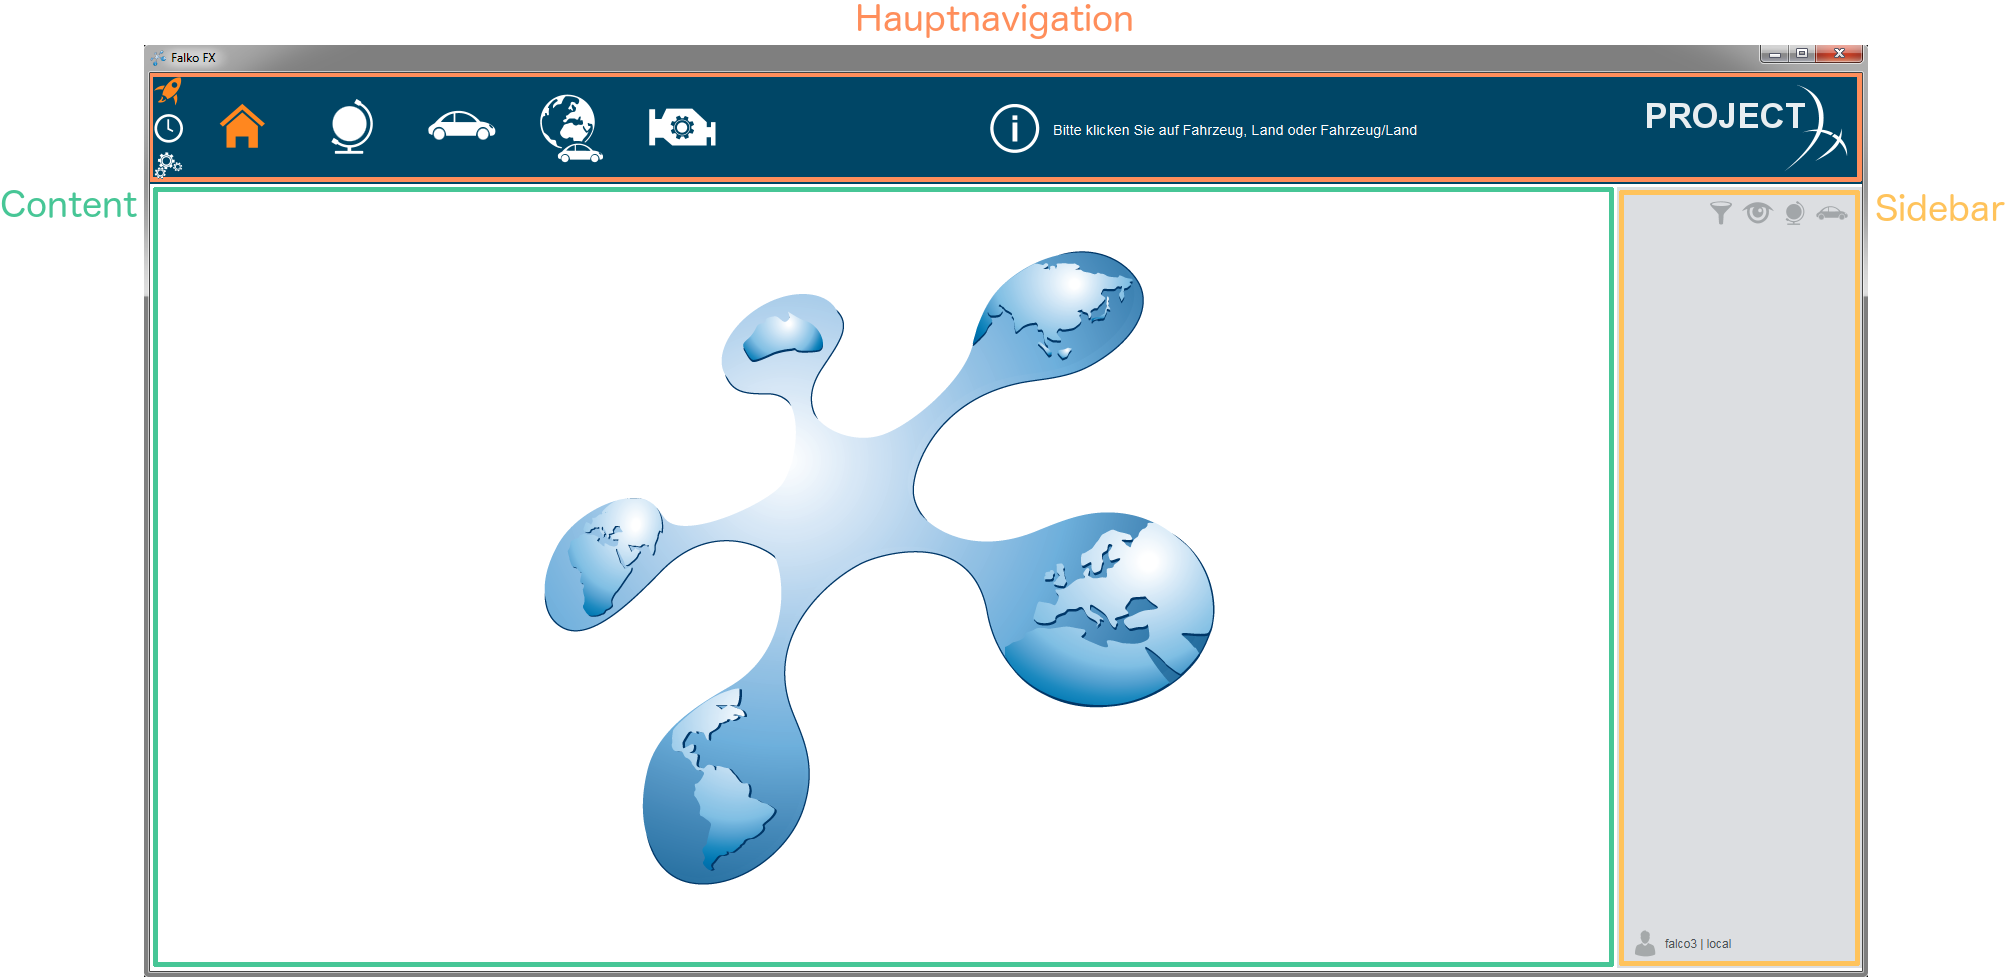
\includegraphics[width=0.8\textwidth]{grafiken/areas.png}
 \caption{Bereiche in FalkoFX}
 \label{fig:areas}
\end{figure}
Das Konzept der gemeinsamen Region wird hier durch die verschiedenen Hintergrundfarben realisiert und unterstreicht die unterschiedlichen Funktionalitäten.\par
\heading{Navigation}
Im Navigationsbereich findet sich im initialen Zustand die Hauptnavigation wieder. Durch die Bedienelemente an der linken Seite der Leiste kann zwischen folgenden Funktionen gewechselt werden:
\begin{enumerate}
	\item Hauptnavigation: Wechsel zwischen Standard-Anwendungsfällen und der verschiedenen Ansichten
	\item Versionsvergleich: Navigation für Anwendungsfälle mit Versionsvergleich (derzeit in Entwicklung und daher nicht weiter betrachtet)
	\item Einstellungen: Menü zum Verwalten anwendungsspezifischer Einstellungen
\end{enumerate}
\begin{figure}[H]
 \centering
 
\includegraphics[width=0.05\textwidth]{grafiken/ribbon.png}
 \caption{Umschalten der Navigation}
 \label{fig:ribbon}
\end{figure}
Durch die vertikale Orientierung, der geringeren Größe und der Nähe zueinander heben sich die Elemente zum Umschalten der Navigation deutlich von den anderen Schaltflächen ab. Wird eines der Elemente angewählt, wird eine Aktion ausgeführt und die Kindelemente, falls vorhanden, werden mittels Animation sichtbar. Die nachfolgenden Elemente der höher liegenden Ebenen werden \enquote{zur Seite geschoben}.\par
\begin{figure}[H]
 \centering
 
\includegraphics[width=0.85\textwidth]{grafiken/navi.png}
 \caption{Navigationshierarchie}
 \label{fig:navi}
\end{figure}
Die Elemente einer einzigen Navigationsebene benötigen keine weitere Trennung. Durch den Freiraum zwischen diesen ist eine hinreichende Trennung erwirkt. Zwischen den verschiedenen Ebenen wird zusätzlich zu einer Farbabstufung eine weiße Trennlinie eingeblendet, die auf der linken Seite einen angedeuteten Pfeil enthält, der die Navigationshierarchie verdeutlicht. Dazu trägt ebenfalls die bereits erwähnte Animation bei.\par
Das Piktogramm des selektierten Navigationselementes wird orange eingefärbt, um die Orientierung zu gewährleisten. Es genügt ein kurzer Blick auf die Navigationsleiste, um festzustellen, welcher Bildschirm gerade aktiv ist, da das Element nach dem Gesetz der Prägnanz heraussticht. Kann der Nutzer eine bestimmte Interaktion nicht ausführen, erscheint das Icon erwartungsgemäß ausgegraut.\par
Durch das Anklicken eines Icons wird der neue Bildschirm angezeigt. Dies geht oft mit dem Laden von Daten einher. Sollten Daten aus der Datenbank geladen werden müssen, wird währenddessen eine Ladeanimation angezeigt. Andernfalls wird der Bildschirm in weniger als 500 Millisekunden angezeigt, wodurch kein weiteres Feedback von Nöten ist. Im Gegenteil: Eine kurz aufblitzende Ladeanimation würde den Anwender eher irritieren als unterstützen.\par
Den Einstieg in jeden Anwendungsfall bietet der Filter. Der Filter besteht in der simpelsten Variante aus folgenden Komponenten:
\begin{itemize}
	\item \textbf{Radial-Menü:} Ein rundes Menü, in dem die zu filternden Attribute ausgewählt werden können
	\item \textbf{Multi-Level-Liste:} Eine mehrstufige Liste mit Suchfunktion, aus der Werte zu den Attributen angewählt werden können
	\item \textbf{Filterselektion:} Eine Liste, welche die aktuell ausgewählten Werte gruppiert darstellt und das Abwählen dieser Werte erlaubt
\end{itemize}
\begin{figure}[H]
 \centering
 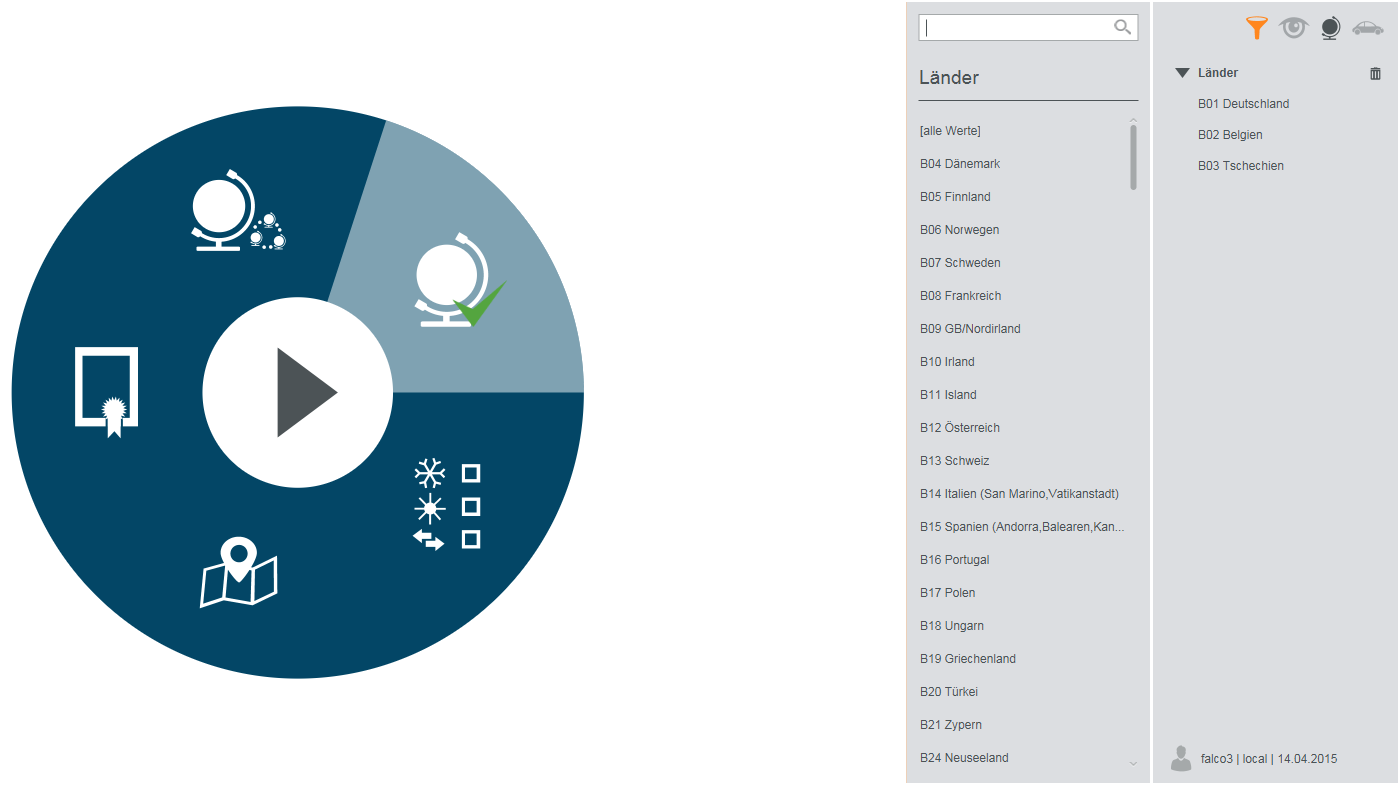
\includegraphics[width=0.6\textwidth]{grafiken/filter_short.png}
 \caption{Beispiel Filter}
 \label{fig:filter}
\end{figure}
Im Radial-Menü sind die Elemente kreisförmig um einen \textit{Play}-Button angeordnet, der standardmäßig deaktiviert ist. Erst, wenn die Ergebnismenge, die durch die gefilterten Attributwerte erzeugt wird, valide ist, wird der Button und das dazugehörige Navigationselement in der Navigationsleiste aktiviert. Die aktuelle Selektion in dem Menü wird durch einen helleren Kreisausschnitt über dem entsprechenden Element markiert. So wird dieser Bereich deutlich hervorgehoben.\par
Die Multi-Level-Liste enthält Werte, die als Filterkriterium ausgewählt werden können. Einige dieser Werte gruppieren weitere Werte und können nicht übernommen werden. Stattdessen öffnet sich beim Auswählen dieser Elemente eine untergeordnete Ebene der Multi-Level-Liste. Diese Werte sind mit einem Pfeil markiert, der in die gleiche Richtung zeigt, in die auch die nachfolgende Animation verläuft.\par
\begin{itemize}
	\item \textbf{Radial-Menü:} Ein rundes Menü, in dem die zu filternden Attribute ausgewählt werden können
	\item \textbf{Multi-Level-Liste:} Eine mehrstufige Liste mit Suchfunktion, aus der Werte zu den Attributen angewählt werden können
	\item \textbf{Filterselektion:} Eine Liste, welche die aktuell ausgewählten Werte gruppiert darstellt und das Abwählen dieser Werte erlaubt
\end{itemize}
\begin{figure}[H]
 \centering
 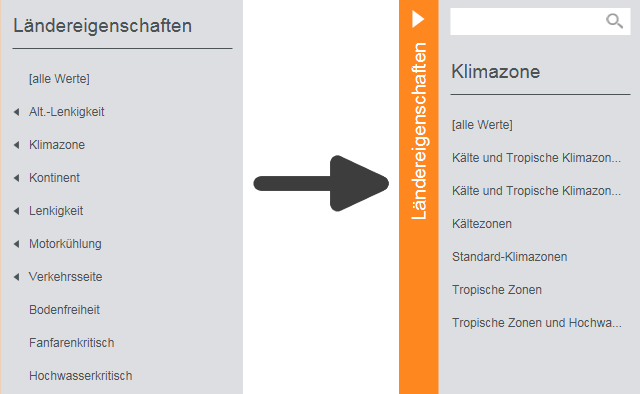
\includegraphics[width=0.4\textwidth]{grafiken/mll_combined.png}
 \caption{Multi-Level-Liste}
 \label{fig:mll}
\end{figure}
Nach dem Filtern der Daten lassen sich die Ergebnisansichten öffnen. Eine Präsentationsmöglichkeit ist die Tabellenansicht. Es handelt sich hierbei um eine komplexe Tabelle, die sämtliche Informationen darstellt. Die Spalten entsprechen den Attributen, zu denen erlaubte Werte im Filter ausgewählt wurden. Zusätzlich sind diese Attribute gruppiert. Die Trennung der Gruppen erfolgt durch deutlich sichtbare Linien, die vertikal zwischen den Spalten der einzelnen Gruppen verlaufen. Die einzelnen Gruppen lassen sich über Bedienelemente in der Sidebar aus- und einblenden, sowie per Drag\& Drop-Geste in der Reihenfolge vertauschen. Der um 45$^{\circ}$ geneigte Spaltenkopf sorgt für eine kompaktere Darstellung, da die minimale Spaltenbreite so nicht mehr durch den Titel der Spalte bestimmt wird. Besonders hilfreich ist diese Präsentation der Spaltenköpfe bei Werten, die nur sehr kurze Bezeichner annehmen. Der Beginn der gedrehten Beschriftungen ist dabei auf einer gedachten horizontalen Linie angeordnet. Auch in diesem Fall lässt sich das Gesetz der Kontinuität anwenden, wodurch die Überschriften als eine zusammengehörige Einheit wahrgenommen werden.\par
\begin{figure}[H]
 \centering
 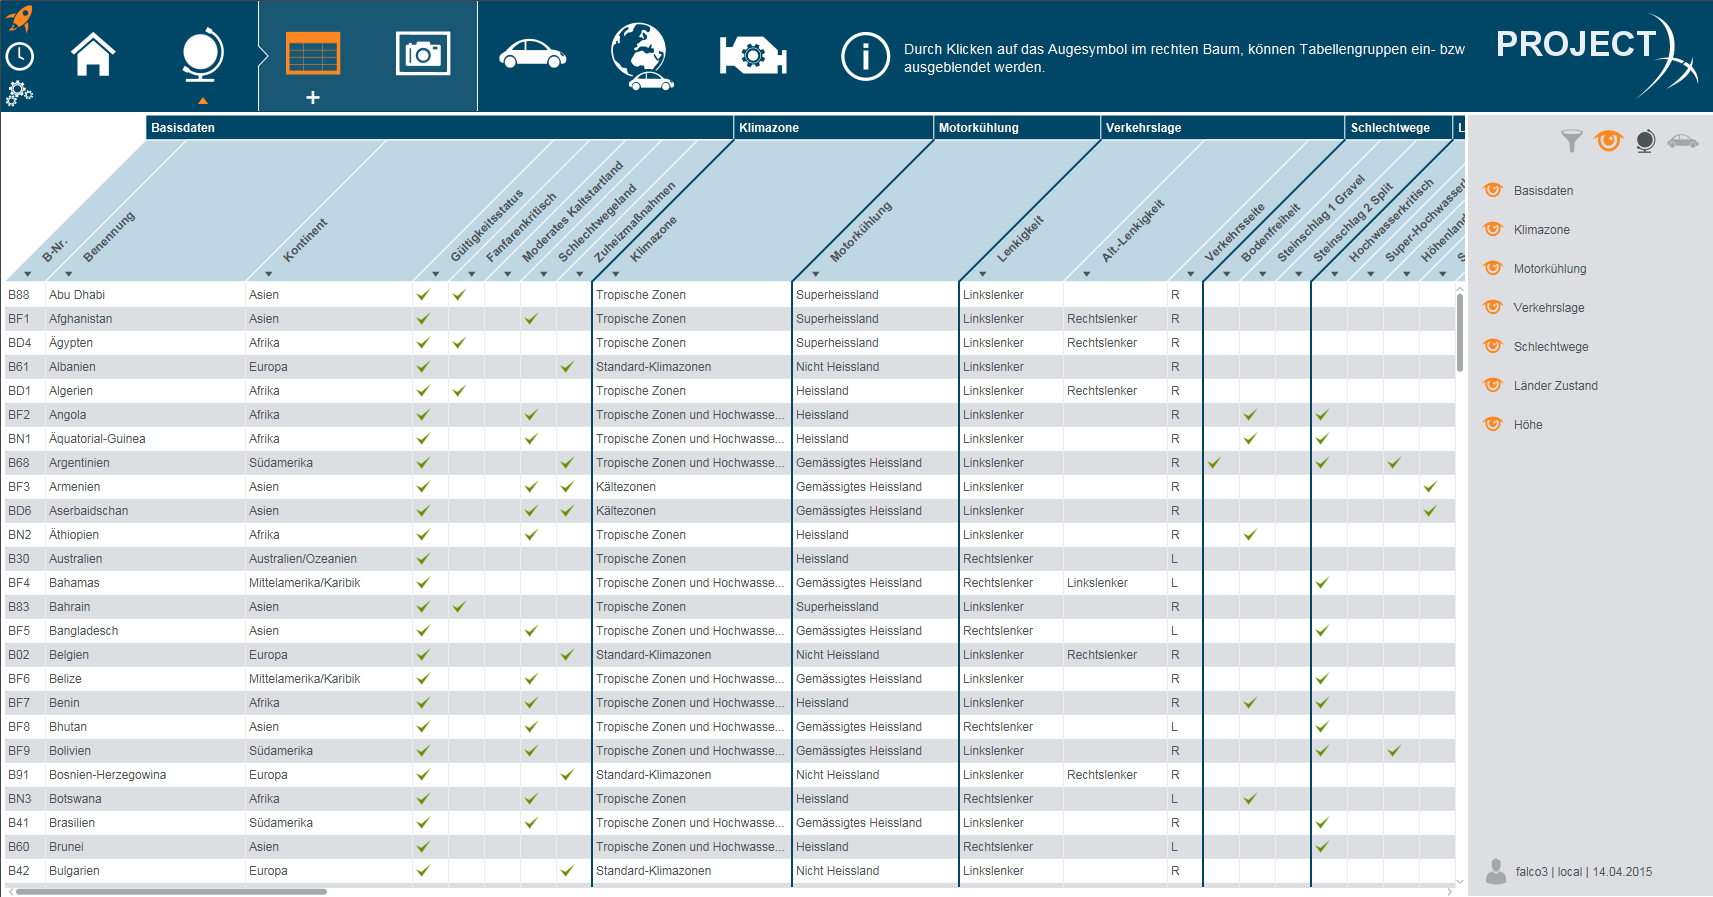
\includegraphics[width=0.6\textwidth]{grafiken/full_result_table.png}
 \caption{Ergebnistabelle}
 \label{fig:resultTable}
\end{figure}
Über die Pfeile im Spaltenkopf lässt sich ein \textit{Overlay} einblenden, in dem die präsentierten Daten auf einfache Weise zusätzlich eingeschränkt werden können, falls mit den aktuellen Einstellungen mehr Datensätze als gewünscht angezeigt werden. Zwar könnten die Pfeile als Elemente zur Umsortierung missverstanden werden, allerdings ist dies kein kritisches Problem, da sich das Overlay nach kurzer Zeit (oder nach dem Verlassen des Bereiches mit dem Mauscursor) schließt und andere Schaltflächen während der Anzeige nicht blockiert werden.\par
\begin{figure}[H]
 \centering
 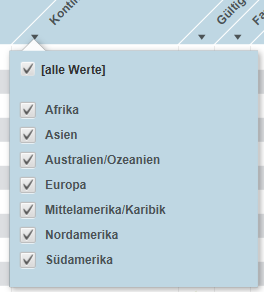
\includegraphics[width=0.3\textwidth]{grafiken/overlay.png}
 \caption{Schnellfilter-Overlay}
 \label{fig:autofilter}
\end{figure}
Im Navigationsbereich ist unter der Schaltfläche der Ergebnispräsentation ein zusätzliches Icon (\ding{58}) aufgetaucht. Bei Klick auf den Bereich des zusätzlichen Icons öffnet sich, mit einer \enquote{Aufklapp-} Animation ein untergeordnetes Menü, das erweiterte Optionen für die derzeit aktive Ansicht bereitstellt. Darunter fallen die Export-Möglichkeiten in PDF und Excel. Die Animation verdeutlicht die Zugehörigkeit zu dem Menüpunkt des aktuell ausgewählten Elements.\par% Als ein mögliches Problem könnte sich das Auftauchen des Icons erweisen. Da der Menüpunkt schon vorher sichtbar war, wird die Änderung ggf. nicht wahrgenommen und ignoriert. Es wird also das Prinzip der Sichtbarkeit nicht vollständig erfüllt.\par
Eine weitere mögliche Ergebnispräsentation ist die Galerie. Hier werden im oberen Bereich Vorschaubilder für Daten angezeigt und darunter eine Detailansicht zum aktuell ausgewählten Element. Mit der Hilfe von $\blacktriangleright$ - und $\blacktriangleleft$ - Schaltflächen lassen sich die Objekte animiert durchschalten. Die aktuelle Selektion wird dadurch verdeutlicht, dass sich dass entsprechende Element stets mittig über der Detailansicht befindet. Zusätzlich wird ein Bezeichner in orangener Schrift darüber angezeigt und das Element wird durch Vergrößerung hervorgehoben. Alle anderen Elemente rücken durch eine geringe Opazität, also einer geringeren Deckkraft, in den Hintergrund. Das Gesetz der Prägnanz wird hier durch mehrere ausschlaggebende Faktoren erfüllt und zeigt dem Anwender unmissverständlich die aktuelle Selektion an.\par
\begin{figure}[H]
 \centering
 \setlength{\fboxsep}{0pt}
 \setlength{\fboxrule}{0.5pt}
 \fbox{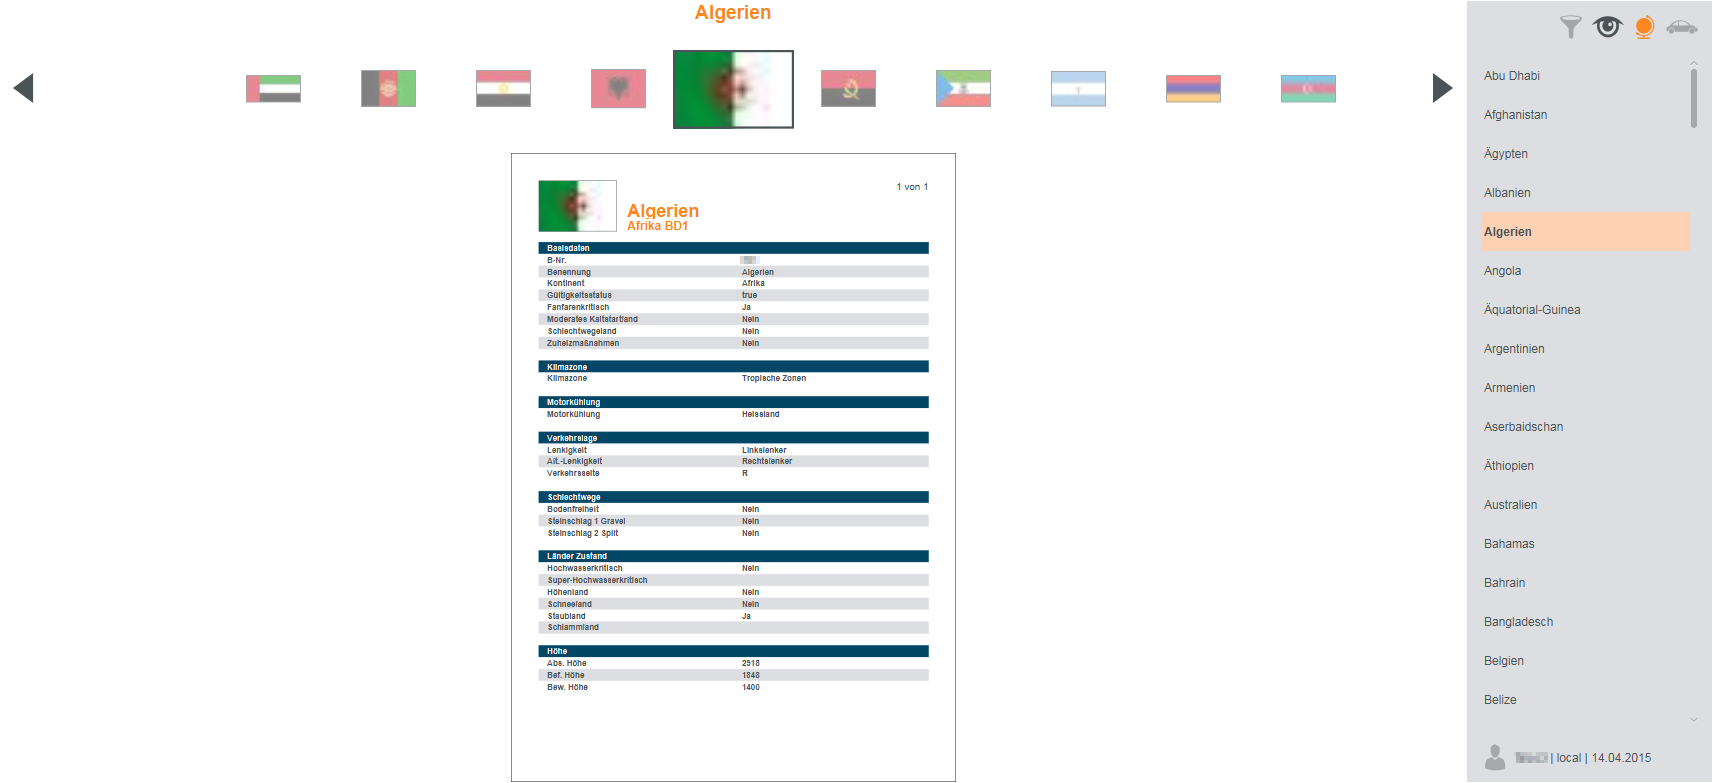
\includegraphics[width=0.6\textwidth]{grafiken/gallery.png}}
 \caption{Galerie}
 \label{fig:gallery}
\end{figure}
Für diese Ansicht ist in der Sidebar standardmäßig die \textit{Ergebnisvorschau} eingeblendet. Diese Ansicht bietet einen Überblick über alle Datensätze, die den Filterkriterien entsprechen. Die Selektion in dieser Liste ist mit der Selektion der Galerie-Komponente gekoppelt und wird so synchron gehalten. Auch die \textit{Ansichtskonfiguration}, die bereits aus der Tabellenansicht bekannt ist, kann hier angewählt und verändert werden. Daraufhin ändern sich die in der Detailansicht der Galerie dargestellten Attributgruppen.\par
Ein Klick auf die Detailansicht öffnet eine vergrößerte Darstellung, den sogenannten \textit{Lesemodus}. Er bietet die Möglichkeit, die zuvor dargestellten Informationen durch die größere Darstellung besser lesen zu können. Die vorherigen und nachfolgenden Datensätze werden durch perspektivisch verschobene Seiten links und rechts der aktuell selektierten Seite eingeblendet. Durch Anklicken lassen sich diese, ebenfalls animiert, in den Vordergrund holen, während die aktive Seite \enquote{wegblättert}. Im Hintergrund verändert sich das selektierte Element in der Galerie. Durch das Anklicken des selbsterklärenden Tür-Icons in der unteren rechten Ecke lässt sich der Lesemodus wieder schließen.\par
\begin{figure}[H]
 \centering
 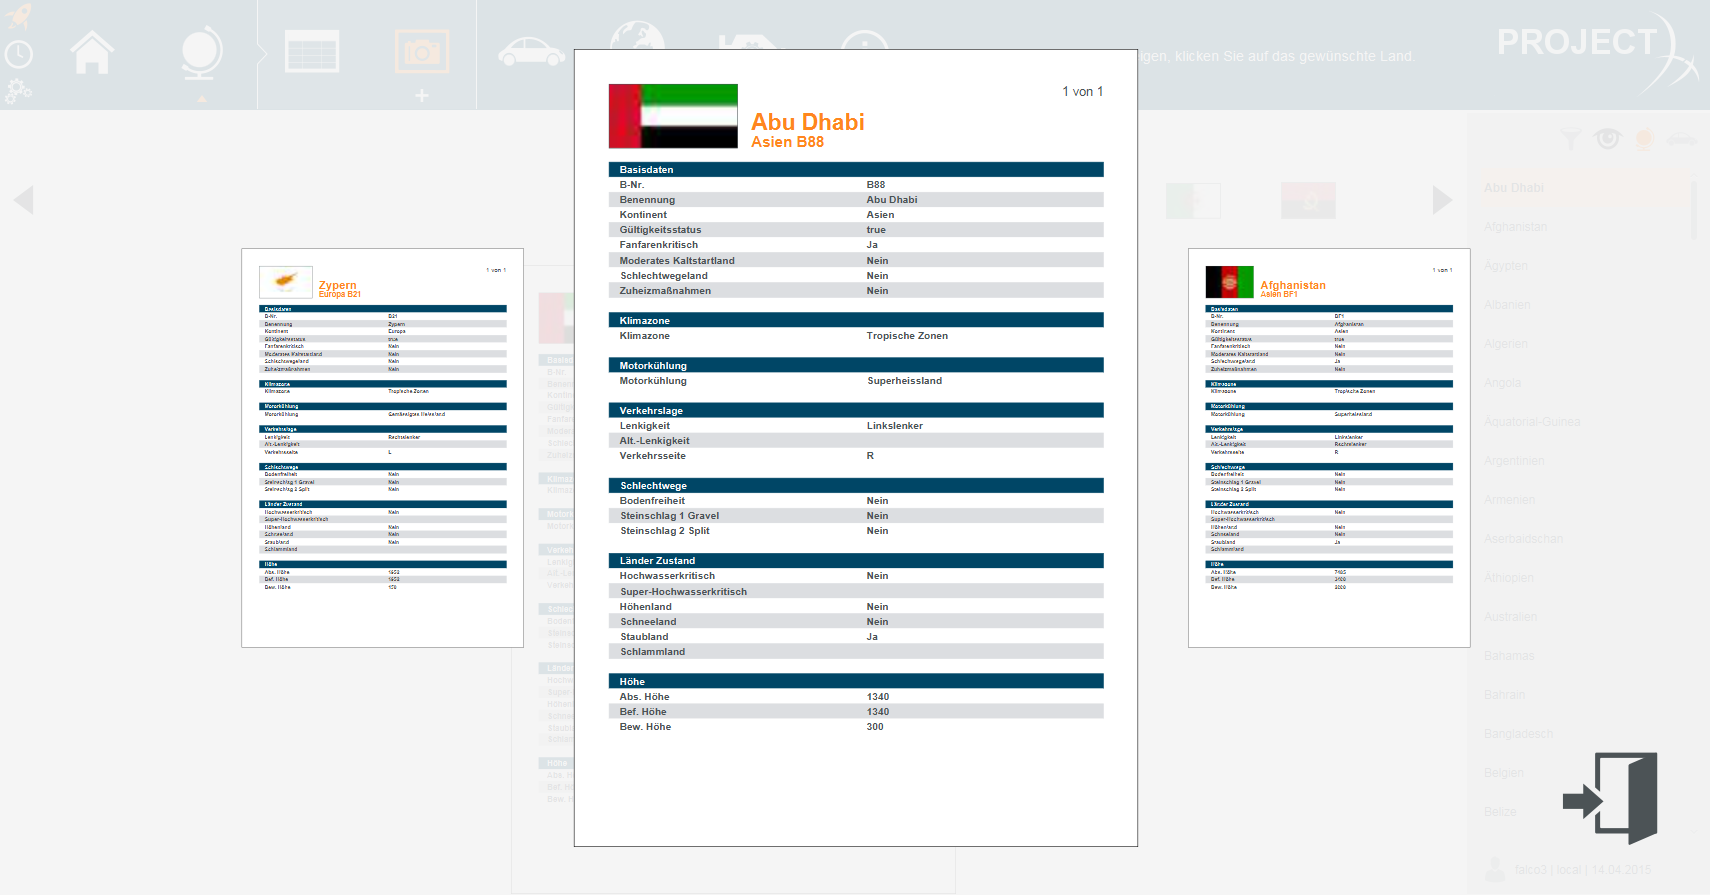
\includegraphics[width=0.6\textwidth]{grafiken/readmode.png}
 \caption{Lesemodus}
 \label{fig:readmode}
\end{figure}
Für den Anwendungsfall der Ländertypenübersicht (kurz: LTÜ) gibt es spezialisierte Filter- und Ergebnisansichten. Der Filter muss verschiedene Modelobjekte verwalten um die Daten der kombinierten Ergebnismenge anzeigen zu können. Daher existieren zwei unterschiedliche Filter-Menüs, die sich mittels Buttons umschalten lassen. Die Buttons sind so gestaltet, dass sie der schematischen Darstellung des RadialMenüs entsprechen und ein Piktogramm der zugrundeliegenden Objekttypen enthalten. So besitzen auch diese Elemente eine Selbsterklärungsfähigkeit.
\begin{figure}[H]
 \centering
 
\includegraphics[width=0.2\textwidth]{grafiken/filter_buttons.png}
 \caption{Filter umschalten}
 \label{fig:filterButtons}
\end{figure}
Die Ergebnispräsentation in diesem Anwendungsfall unterscheidet sich von der der anderen Anwendungsfälle. In der Ergebnistabelle werden die Daten in einer \textit{Matrixdarstellung} visualisiert. Die Zeilen werden zu Beginn mit den konfigurierbaren Informationen der Fahrzeugdaten befüllt. Danach werden weitere Spalten erstellt, die mit den einzelnen Ländern aus den gefilterten Länderdaten gekennzeichnet sind. Auf diese Weise ergibt sich eine Matrix aus Freigabedaten für jede mögliche Fahrzeug-Länder-Kombination. Durch die unterschiedliche Gestaltung des Spaltengruppenkopfes heben sich die Länderspalten von den Spalten mit den Fahrzeugattributen visuell ab und definieren so einen eigenen Abschnitt.
\begin{figure}[H]
 \centering
 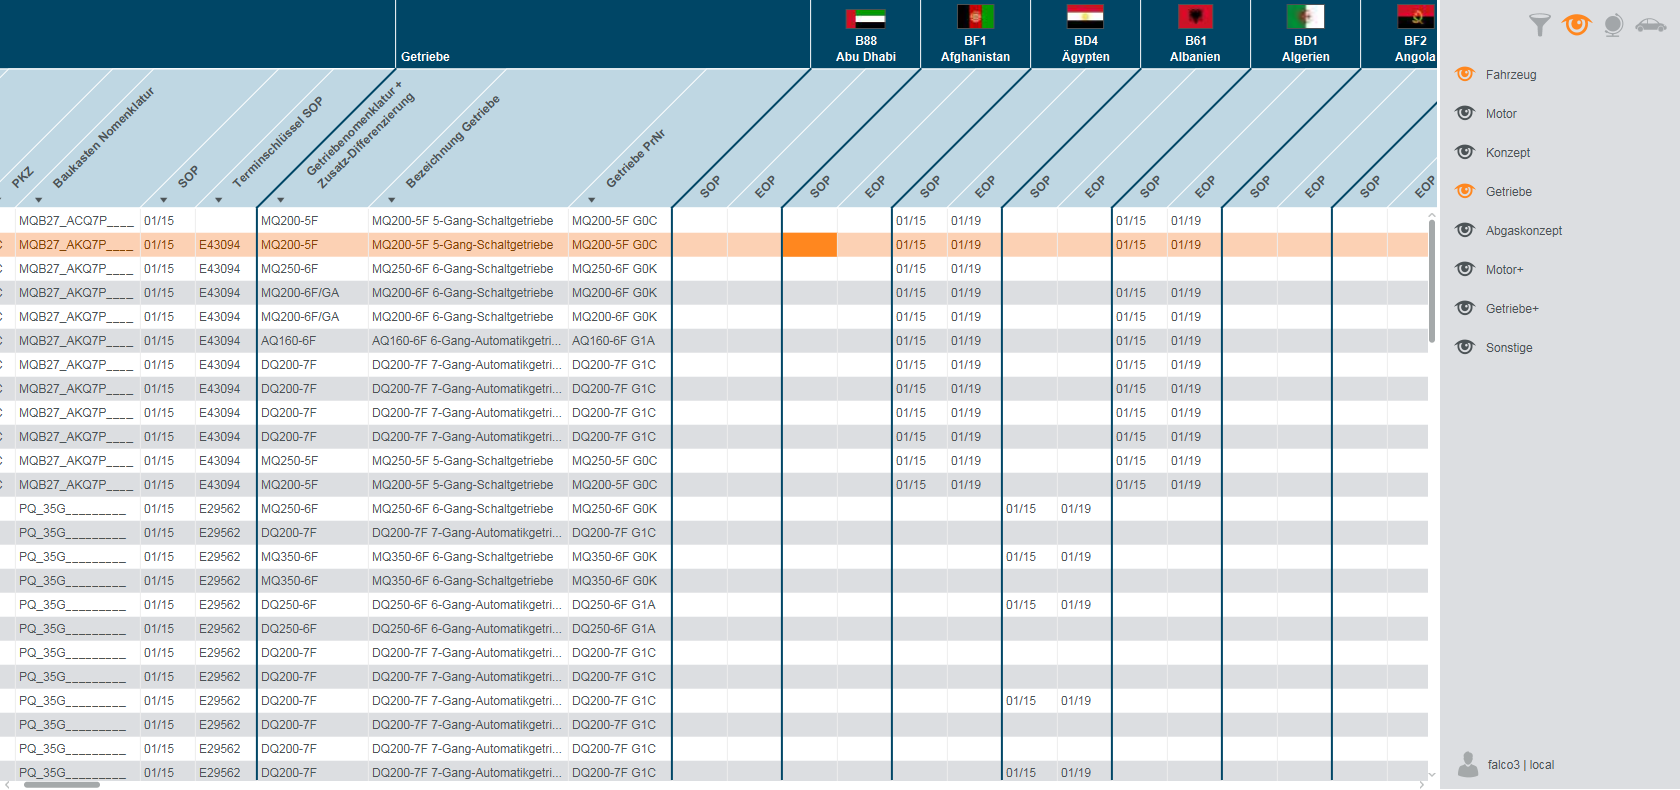
\includegraphics[width=0.6\textwidth]{grafiken/ltue_table.png}
 \caption{LTÜ Ergebnistabelle}
 \label{fig:ltueTable}
\end{figure}
Die Selektion findet zellenweise statt. Durch einen Doppelklick auf eine einzelne Freigabe können Details zu dieser Freigabe eingeblendet werden. Dennoch wird die Hintergrundfarbe der gesamten Zeile, in der sich die Selektion befindet, angepasst, damit die Orientierung in der komplexen Tabelle erleichtert wird. Das aktuell selektierte Fahrzeug ist so stets erkennbar, selbst, wenn die selektierte Freigabe nicht sichtbar ist.\par
Die Detailansicht zu einer Freigabe wird, anders als beim Lesemodus, nur im Content-Bereich der Applikation angezeigt. Hier wird für die Darstellung der Informationen weit weniger Platz benötigt, weshalb diese Darstellungsform ausreicht. Die Navigations- und die Seitenleiste sind weiterhin sichtbar, allerdings ist in der Sidebar keine Ansicht auswählbar und so wird diese leer angezeigt. Der Vorteil an der kontinuierlichen Sichtbarkeit der Navigationsleiste ist, dass der Kontext nicht verloren geht. Der Nutzer weiß also immer, wo er sich befindet, und welche Ansicht angezeigt wird, wenn er die Detailansicht wieder verlässt. Dies ist wichtig, da sowohl von der Tabellenansicht als auch von der Listenansicht, der weiteren verfügbaren Ergebnispräsentation, zu den Details einer Freigabe navigiert werden kann.\par
\begin{figure}[H]
 \centering
 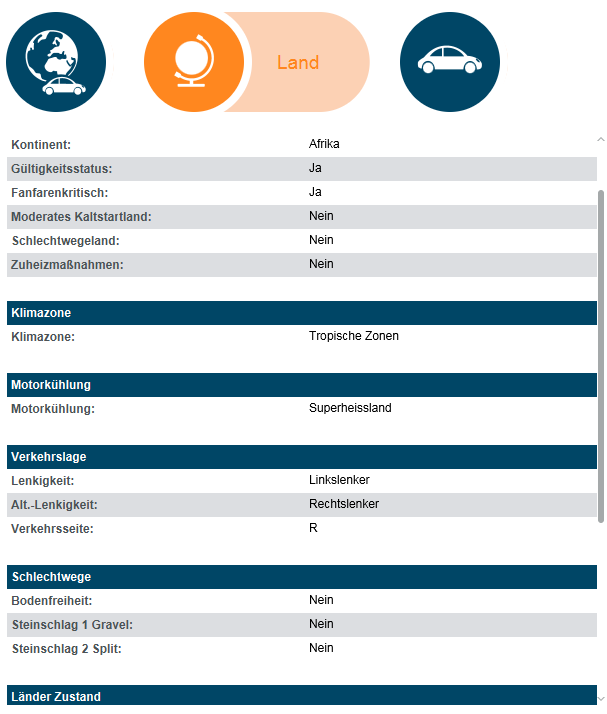
\includegraphics[width=0.3\textwidth]{grafiken/ltue_details.png}
 \caption{LTÜ Detailansicht}
 \label{fig:ltueDetails}
\end{figure}
Die Listenansicht ist eine zweigeteilte Darstellung. Auf der linken Seite befindet sich eine Tabelle mit den Fahrzeugen der Ergebnismenge als Inhalt. Auf der rechten Seite werden alle gefilterten Länder angezeigt, zu denen für das links ausgewählte Fahrzeug eine Freigabe existiert. Da der Inhalt der linken Tabelle deutlich umfangreicher ist, nimmt diese Seite mehr Platz ein als die Länderliste. Durch Doppelklick auf das entsprechende Land können die Details der Freigabe eingesehen werden.\par
\begin{figure}[H]
 \centering
 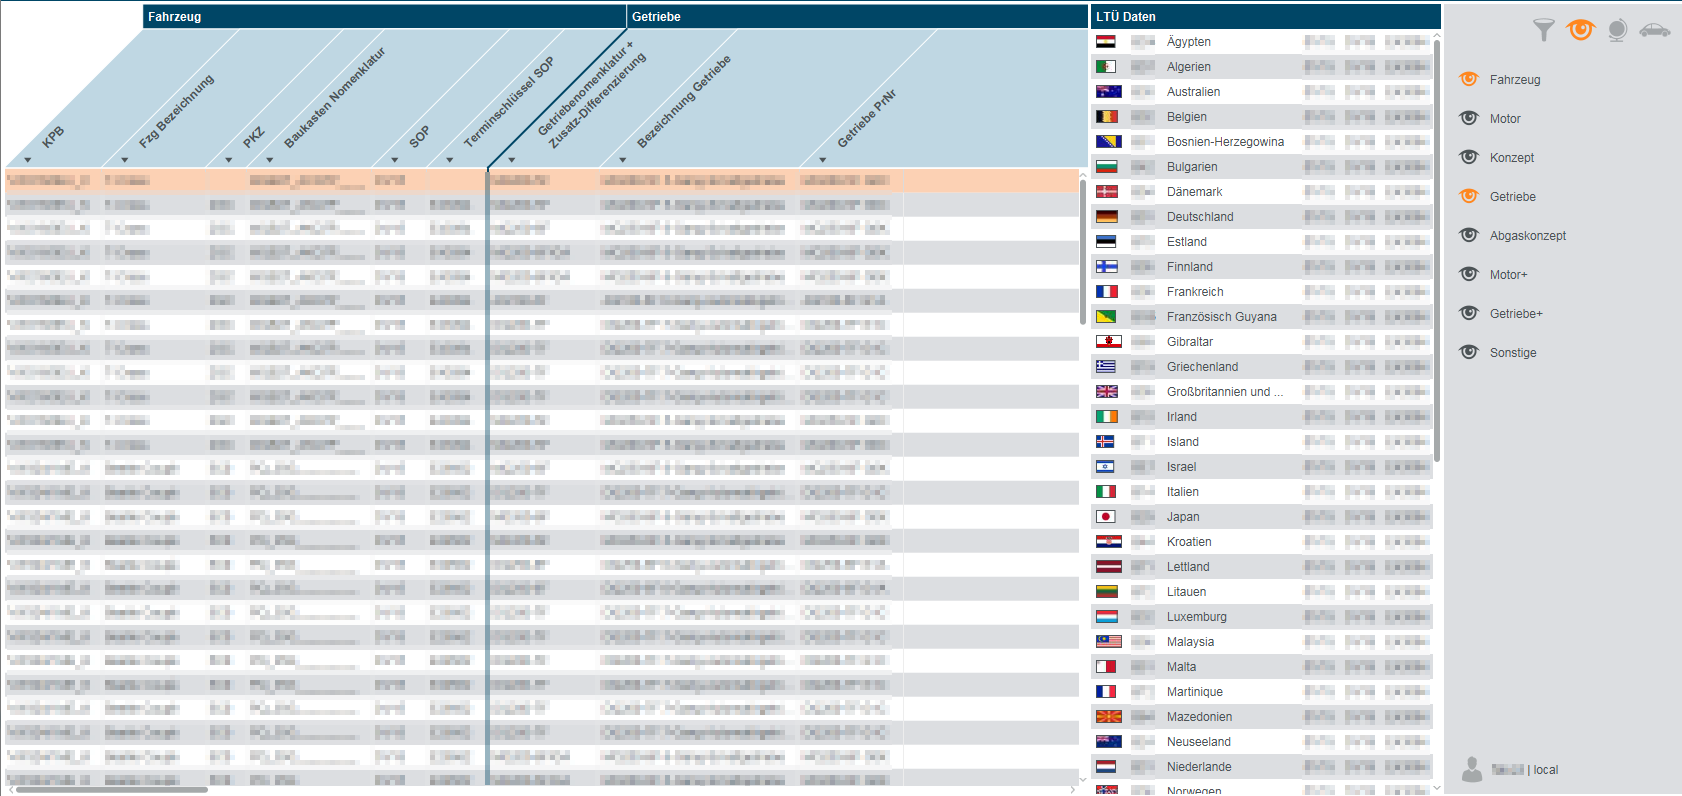
\includegraphics[width=0.6\textwidth]{grafiken/ltue_list.png}
 \caption{LTÜ Listenansicht}
 \label{fig:ltueList}
\end{figure}
Durch die Ähnlichkeit der beiden Komponenten wird die Zusammengehörigkeit schnell deutlich. Dieser Effekt wird zum einen durch die gleich gestalteten Zeilen erwirkt (Wechsel zwischen weißer und grauer Zeile) und zum anderen durch die aneinander ausgerichteten Kopfelemente. Dies sind der Spaltengruppenkopf der Tabelle und die \enquote{Überschrift} der Länderliste.\par
\subsection{Tastaturbedienbarkeit}
Die Anwendung ist momentan nur per Maus bedienbar. Die Möglichkeiten der Tastatur, die an jedem Arbeitsplatz zu finden ist, werden nicht ausgenutzt. Die Identifikation der Anwendungsbereiche, in denen die Tastatur eine alternative Bedienmöglichkeit darstellen kann, ist Ziel dieses Abschnittes. Dabei wird ein grundlegendes Konzept entworfen, für das in Abschnitt \ref{sec:designInteraction} spezialisierte Designlösungen gefunden werden.\par
Die erste Komponente, für die eine Tastatursteuerung denkbar wäre, ist die Navigation. Dabei sollten sowohl die Schaltflächen für das Umschalten der Navigationsleiste, als auch die Elemente per Tastatur bedienbar sein. So ist die grundlegende Steuerung der Anwendung möglich. Für die einzelnen Bildschirme müssen jeweils spezialisierte Lösungen gefunden werden.\par
Der erste Bildschirm, zu dem navigiert werden kann, ist in jedem Anwendungsfall der Filter. Hier gibt es das Radialmenü, die mehrstufige Liste und die Sidebar mit den gewählten Filterkriterien. Primär sollte die Liste mit der Tastatur bedient werden können, mit dem Ziel, Werte möglichst schnell zu finden und auszuwählen. Weiterführend kann die Steuerung für das Radialmenü umgesetzt werden, damit die Werte über verschiedene Attribute hinweg per Tastatur auswählbar sind. Die Bedienung der Sidebar ist eher nachrangig, da ihr Zweck ist, ausgewählte Werte wieder deselektieren zu können - folglich \enquote{nur} ein Mittel, um Fehler zu korrigieren.\par
In der Tabellenansicht, die in jedem Anwendungsfall verfügbar ist, ist eine Steuerung der Selektion denkbar. Außerdem sollte von einem Element zu den dazugehörigen Details gesprungen werden können, ohne dabei zur Maus wechseln zu müssen. Eine Steuerung der Sidebar wäre nur für den Reiter der Ansichtskonfiguration von Nöten, da die anderen verfügbaren Ansichten nur der Ergebnisvorschau dienen.\par
Ähnlich ist die Situation bei der Galerie. Auch hier wäre eine Tastatursteuerbarkeit der Galerie, inklusive Öffnen der vergrößerten Ansicht im Lesemodus vorteilhaft. Das Durchschalten der Elemente kann ebenfalls mit der Tastatur erfolgen. Das Konzept dafür sollte nach Möglichkeit in allen Ergebnispräsentationen ähnlich sein. So sollte auch der Lesemodus nach dem gleichen Schema behandelt werden.\par
Die Listenansicht des LTÜ-Anwendungsfalles benötigt auch ein vergleichbares Konzept zur Steuerung. Die Schwierigkeit besteht darin, dass prinzipiell zwei Kontrollelemente gleichzeitig steuerbar sein müssen.\par
%Bei der Detailansicht, die von der Ergebnistabelle und der Listenansicht erreichbar ist, ist eine Unterstützung der Subnavigation (Wechsel zwischen LTÜ-, Land- und Fahrzeugdaten) in diesem Bildschirm denkbar.\editHere{Wenn hier, dann auch in Impl}\par
\subsection{Übertragung von Touchgesten auf Maussteuerung} \label{sec:analyseGesten}
Mit Blick auf den immer stärker werdenden Trend, auch Geschäftsanwendungen auf mobile Geräte zu portieren, soll an dieser Stelle geprüft werden, inwiefern die Touchgesten (vgl. Kapitel \ref{fig:touchGestures}) auf das Bedienkonzept am Desktop-PC übertragbar sind. Dies soll zum einen zu einer intuitiveren Bedienung mit der Maus beitragen und zum anderen für die Benutzung der Software auf Convertibles vorsorgen.\par
Der Mauszeiger wird zu diesem Zweck als \enquote{Ersatz} für den Finger auf einem Touch-Display verwendet. Da es nur einen Mauszeiger und eine Maus gibt, ist es technisch gesehen nur möglich, Gesten durchzuführen, die genau einen Finger benötigen. Dies sind \textit{Tap}, \textit{Double Tap}, \textit{Drag}, \textit{Flick} und \textit{Press}. Die \textit{Tap} und \textit{Double Tap}-Gesten entsprechen sowohl von der Durchführung, als auch von der Semantik in der Regel dem einfachen Mausklick bzw. dem Doppelklick. Die \textit{Drag}-Geste ist der Drag\& Drop Aktion der Maus sehr ähnlich. An vielen Stellen jedoch, an denen bei mobilen Anwendungen \textit{Drag}-Gesten verwendet werden würden, wird die Benutzung eines UI-Elements auf dem Desktop-PC mit anderen Mitteln gelöst. Für den \textit{Flick}, auch \textit{Swipe} genannt, existiert kein Pendant im Pensum der normalen Maus- und Tastatur- Interaktion. Dennoch ist es denkbar, eine solche Geste mit einer schnell ausgeführten Drag\& Drop-Aktion zu ermöglichen. Auch der \textit{Press} kann mit den gegebenen Eingabemitteln umgesetzt werden. Eine solche Aktion ist jedoch in den meisten Fällen nur bedingt intuitiv verwendbar, da keine ähnlichen, dem Nutzer vertrauten, Aktionen für die Maussteuerung existieren. Als Ersatz kann der Rechtsklick bei der Desktop-Verwendung genutzt werden.\par
Die erste Komponente, für die eine Gesten-Unterstützung untersucht wird, ist die Navigationsleiste. Hier ist jedes aktive Element durch einen einfachen Mausklick verwendbar. Dieses Verhalten entspricht dem, was Nutzer mobiler Anwendungen bei der Bedienung erwarten würden. \textit{Swipe} oder \textit{Drag}- Gesten würden hier eher zu Verwirrung führen.\par
Die Bedienung des Radialmenüs im Filter ist zunächst nur mit einfachen Klicks auf die Zielelemente möglich. Als Alternative dazu sollten auch Touchgesten und deren Pendant auf Desktop-PCs bereitgestellt werden. Bei der Bedienung der Liste wird sich bislang auf das Scrollrad und den Scrollbalken verlassen. Auf Geräten, die nativ Toucheingaben unterstützen, ist das Scrolling per \textit{Drag} nativ bereits unterstützt. Um das Verhalten auf verschiedenen Plattformen anzugleichen und die Spanne von unterstützten Eingabemethoden zu erhöhen, sollte die Bedienmöglichkeit auch für die Maus umgesetzt werden. Durch diese Art von Scrolling kann vorallem in langen Listen genauer und zielgerichteter zu gesuchten Einträgen gelangt werden.\par %Sidebar?
In den Ergebnisansichten, in denen eine Tabelle bzw. eine Liste verwendet wird, stellt sich ein vergleichbares Problem. Jegliche Art von Tabelle oder Liste kann mit einer \textit{Drag}-Geste gescrollt werden, wenn die Eingabe über ein Touch-Display erfolgt. Die Steuerung sollte auch an diesen Stellen an die Touch- Bedienung angepasst werden. Dies sind im Speziellen die Ergebnistabelle und die Listenansicht.\par
In der Galerie muss die Umsetzung auf eine eigene Weise erfolgen. Die Leiste, in der die Vorschaubilder der angezeigten Datensätze angezeigt werden, kann ebenfalls mit neuen Bedienungsmöglichkeiten versehen werden, um die aktuelle Selektion zu verändern. Eine Steuerung, die nur über die Buttons links und rechts der Bordüre abgehandelt wird, schränkt den Nutzer stark ein. Ein ähnliches Verhalten zeigt der Lesemodus. Hier lässt sich das zentrierte, vergrößerte Datenblatt nur durch Anklicken eines der seitlichen Datenblätter ändern.\par
Zu guter Letzt existiert noch eine tabellenartige Komponente in der Detailansicht des LTÜ-Anwendungsfalles. Werden in der Komponente genügend Daten angezeigt, muss auch diese per Gesten gescrollt werden können.\par
\section{Design} \label{sec:designInteraction}
Nachdem die relevanten Stellen in der Analysephase aufgedeckt wurden, werden in diesem Abschnitt konzeptionelle Lösungen entwickelt, nach denen die Umsetzung erfolgen kann.\par
\subsection{Tastaturbedienung} \label{sec:interactionKeyboard}
Das Implementieren der einzelnen Teillösungen ist nicht sinnvoll, ohne zunächst ein Gesamtkonzept entworfen zu haben. Wie in der Analysephase festgestellt, gibt es mehrere Komponenten, für die eine Tastaturbedienung ermöglicht werden soll. Einige dieser Komponenten können zeitgleich auf dem Bildschirm sichtbar sein (z.B. die Navigationsleiste und die mehrstufige Liste der Filteransicht). Das führt in der Bedienung zu Konflikten, da Tastatureingaben, nach dem in Abschnitt \ref{sec:javafxEventhandling} beschriebenen Event-Handling-Konzept, nur an einem spezifischen Knoten im Szenegraphen angelangen, wenn dieser den Eingabefokus besitzt. Es ist demnach nicht möglich, die Events an einem bestimmten Knoten zu behandeln indem der Fokus auf dieses Element gesetzt wird. Das Problem kann jedoch umgangen werden. Anstatt EventHandler an den jeweiligen Komponenten zu registrieren, können die EventHandler direkt an dem \textit{Szene}-Knoten, also der Wurzel des Szenegraphen, angemeldet werden.\par
\heading{Sekundäre Funktionalitäten}
Ein Konzept, das in modernen Anwendungen oft Verwendung findet sind die \textit{Mnemonics}. Mnemonics sind Tastenkombinationen mit denen in der Regel sekundäre Funktionen, wie zum Beispiel Menüs, bedient werden können. Eine Methode, die in modernen Anwendungen Verwendung findet ist das einmalige Drücken der \textit{Alt}-Taste, das die Einblendung der möglichen Tastenkombinationen zufolge hat. Eine ähnliche Umsetzung kann für die Sekundärfunktionen von FalkoFX erfolgen. Dazu zählen vorallem die Navigationsleiste und die Sidebar. Um den Nutzer dabei zu unterstützen, die mit Mnemonics versehenen Elemente zu identifizieren, wird (bei Drücken der \textit{Alt}-Taste) über der gesamten Anwendung eine leicht transparente Komponente eingeblendet, die genau die Stellen ausspart, an denen sich steuerbare Objekte befinden. Zudem wird in den dadurch erzeugten Bereichen die Tastenkombination eingeblendet, welche die entsprechende Aktion ausführt.\par
Für das Steuern der Navigationsleiste eignen sich die Zahlentasten am besten. Die verschiedenen Navigationsleisten werden parallel dazu mit den Funktionstasten F1, F2, etc. umgeschaltet. Um die Sidebar zu bedienen sollten im Optimalfall sprechende Kombinationen gewählt werden. Das wäre beispielsweise der Buchstabe \enquote{E} für Ergebniskonfiguration oder \enquote{F} für die Filterauswahl. Generell gilt: Es sollten nur die Elemente mit Mnemonics versehen werden, die sichtbar, aktiv und auch mit normalen Mausklicks zu verwenden sind.\par
\heading{Filter}
Die Haupteingabe findet immer in dem derzeit im Content-Bereich aktiven Bildschirm statt. Unter diese Bildschirme fällt der Filter. Die damit primär durchgeführte Aktion ist das Auswählen von Attributwerten aus der mehrstufigen Liste. Zu der Liste gehört stets das Schnellfilter-Textfeld im oberen Bereich. Der normale Arbeitsablauf eines Nutzers ist das Anklicken des Textfeldes, eingeben eines Textes und Anklicken des gefundenen Wertes. Um diesen Ablauf möglichst effizient und angenehm zu gestalten sollte der Wechsel von Tastatur zu Maus erspart werden. Dies kann erreicht werden, indem die Eingabe eines Zeichens immer dazu führt, dass das Textfeld den Fokus erhält und der Text dort eingegeben wird, unabhängig davon, welches Element den Fokus derzeit besitzt. Diese Umsetzung ist nur möglich, weil parallel keine Elemente existieren, die eine direkte Eingabe von Text erwarten oder den Eingabefokus benötigen. Weitergehend können die Pfeiltasten der Tastatur für die Navigation in der Liste genutzt werden. Hat der Nutzer einen Text eingegeben und möchte einen gefundenen Wert selektieren, kann er von der Eingabe mit der $\downarrow$- Taste direkt zum ersten Element der Liste springen und darin auf natürliche Weise weiter navigieren. Zu einer untergeordneten Ebene kann mit der $\leftarrow$- Taste gelangt werden und die entgegengesetzte Aktion, das zurückspringen zur übergeordneten Ebene, wird durch $\rightarrow$ bereitgestellt.\par
Die Bedienung des Radialmenüs wird durch die globale Eingabe im Textfeld und die Verwendung der Pfeiltasten für die Liste zwar eingeschränkt, aber auch hier kann das erwähnte Konzept der Mnemonics nach dem gleichen Schema wie in der Navigation verwendet werden. Zwar ist das Radialmenü Teil des angezeigten Bildschirms, gemessen an der Benutzungshäufigkeit ist die Multi-Level-Liste jedoch ein höher priorisiertes Bedienelement. Das Verhalten ist dahingehend konsistent mit dem Gesamtkonzept der Steuerung.\par
\heading{Ergebnisansichten}
Die Ergebnisansichten sollten intuitiv mit den Pfeiltasten der Tastatur steuerbar sein. Bei Zeilenselektion haben nur die $\downarrow$- und $\uparrow$- Tasten einen Effekt. Ist die Zellselektion aktiviert, können die $\leftarrow$- und $\rightarrow$- Tasten für die Navigation durch die Spalten genutzt werden. Würde sich die nächste per Pfeiltaste selektierte Zelle außerhalb des angezeigten Bereiches befinden, muss die Tabelle entsprechend gescrollt werden. Die Enter-Taste kann dazu verwendet werden, um die die dem Anwendungsfall entsprechende Detailansicht des angewählten Datensatzes aufzurufen.\par
Die Galerie kann durch verschiedene Tastatureingaben unterstützt werden. Zum einen kann, genau wie in der Ergebnistabelle, per Pfeiltasten zwischen den Elementen gewechselt werden, zum anderen können aber auch Freitext-Eingaben zu einer intuitiven Bedienung beitragen. Ist der Galerie-Bildschirm aktiv, kann der Nutzer anfangen, einen Text zu tippen. Solange die Tastendrücke nicht zu lange auseinander liegen, wird der Text mit dem Wert des primären Attributes aller Datensätze verglichen. Anhand des Länderanwendungsfalles würde dies bedeuten, dass der Anwender nach einem bestimmten Land sucht. Anstatt dieses aus der langen Länderliste heraussuchen zu müssen, kann er den Anfang des Namens eintippen und die Galerie scrollt automatisch zu dem gesuchten Element. Ist der Nutzer also auf der Suche nach dem Land \enquote{Deutschland}, tippt er \enquote{Deu} und gelangt noch während des Tippvorganges zu dem Datensatz. Auch hier öffnet die Enter-Taste wiederum die Detailansicht, die in diesem Anwendungsfall durch den Lesemodus repräsentiert wird.\par
Konsistent zu den anderen Ansichten lässt sich im Lesemodus der im Fokus stehende Datensatz mit den Pfeiltasten durchschalten. Drücken der ESC-Taste schließt den Lesemodus erwartungsgemäß. \par
Eine komplett identische Umsetzung dieses Konzeptes ist in der Listenansicht des LTÜ-Anwendungsfalles nicht möglich. Hier gibt es zwei Komponenten, die mit den Pfeiltasten bedient werden müssen. Der Bedienungsablauf ohne Tastatursteuerung wäre der, dass der Nutzer zunächst ein Fahrzeug aus der Tabelle auswählt. Daraufhin werden ihm in der rechtsseitigen Liste alle Länder angezeigt, die zu den Filtereinstellungen passen und für die eine Freigabe des Fahrzeuges existiert. Zwischen der Bedienung dieser beiden Teile der Darstellung sollte gewechselt werden können. Dies kann unter zum Beispiel durch die $\leftarrow$- und $\rightarrow$- Tasten gelöst werden. Standardmäßig sollte jedoch die linke Hälfte der Ansicht im Fokus der Bedienung stehen.\par
%Die Subnavigation der LTÜ-Detailansicht kann unter Verwendung der Pfeiltasten ($\leftarrow$- und $\rightarrow$) bedient werden. Die Selektion würde erwartungsgemäß von e
\subsection{Gestensteuerung}
Das Ziel der Gestensteuerung ist es, dem Nutzer eine intuitive Bedienung der Oberflächenelemente zu ermöglichen. Durch die in Abschnitt \ref{sec:analyseGesten} erläuterten Gesten ist es möglich, die Anwendung auf verschiedenartigen Geräten auf die gleiche Weise zu benutzen. Dabei kann zwischen bereichsabhängigen Gesten (z.B. \textit{Drag}) und unabhängigen Gesten (z.B. \textit{Swipe}) unterschieden werden.
\heading{Filter}
In der Filteransicht sollte sowohl das Radialmenü, als auch die mehrstufige Liste unterstützt werden. Zusätzlich zu der Bedienung des kreisförmigen Menüs durch einfache Klicks, können hier \textit{Drag}-Aktionen für eine barrierefreie Bedienung sorgen. Auf Mobilgeräten ist es häufig möglich, diese Selektion durch eine Geste, statt durch \textit{Tap}s zu ändern. Die Geste beginnt über dem Abschnitt des Menüs, der selektiert ist und wird bis zu dem Abschnitt ausgeführt, der das Ziel darstellt. Dabei ist der Weg der Geste unerheblich und die Selektion folgt ihr. Für eine optimale Erfahrung sollte die Position des Selektionsbereiches nicht abhängig von der Entfernung des Mauszeigers bzw. des Fingers vom Mittelpunkt des Menüs sein. Alleine der Winkel vom Start der Geste bis zum Ziel oder derzeitigen Berührungspunkt/ der derzeitigen Mauszeigerposition ist hierfür ausschlaggebend:\par
\begin{figure}[H]
 \centering
 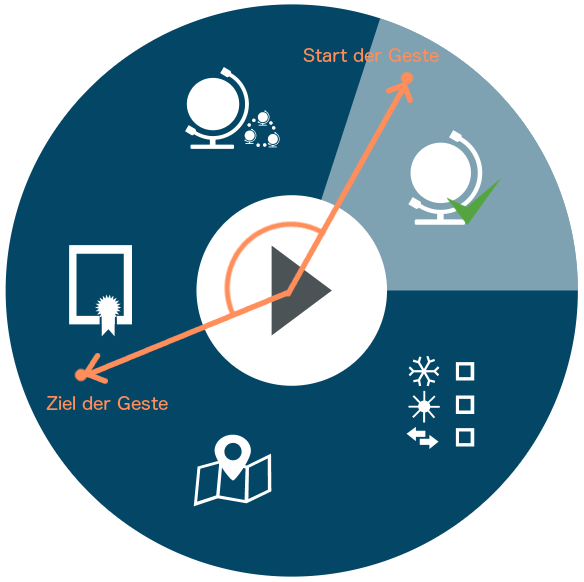
\includegraphics[width=0.45\textwidth]{grafiken/radial_gesture.png}
 \caption{Radialmenü Geste}
 \label{fig:radialGesture}
\end{figure}
Der hell eingefärbte Kreisausschnitt muss sich also um genau den Winkel, der in der beispielhaften Abbildung \ref{fig:radialGesture} zu sehen ist, um den Mittelpunkt des Kreises drehen. Bei jeder Bewegung der Maus sollte die Position des Selektionsbereiches aktualisiert werden. Nach Abschließen der Geste erhält der Menüeintrag die Selektion, in dessen Teilbereich die Winkelhalbierende des Selektions-Kreisausschnittes liegt - also jenes Element, welches zu einem größeren Teil durch den hell eingefärbten Kreisausschnitt bedeckt wird. Dabei wird der Kreisausschnitt durch eine Animation so positioniert, dass er wieder exakt über dem selektierten Element liegt. \par
Für die Liste kann eine \textit{Drag}- Geste zum Scrollen eingeführt werden, die analog zu der nativ vorhandenen mobilen Geste funktioniert. Das bedeutet, die Liste folgt der vertikalen Bewegung des Mauszeigers bzw. des Fingers.\par
\heading{Ergebnisansichten}
Für alle Tabellen und Listen innerhalb der Ergebnisansicht kann das gleiche Konzept angewandt werden, das bereits für die mehrstufige Liste des Filters entworfen wurde. Bei Tabellen muss zusätzlich zu der vertikalen Verschiebung, die horizontale Änderung der Mauszeiger- oder Fingerposition beachtet werden. Die Vorschaubilder in dem Galerie-Bildschirm können ebenfalls als eine Art Liste gesehen werden, welche die Elemente horizontal nebeneinander ausrichtet, daher sollte auch diese Komponente durch \textit{Drag}-Gesten unterstützt werden. Anders als bei den bisherigen Navigationsmethoden innerhalb dieser Komponente wird dadurch ein stufenloses Scrolling ermöglicht. Daher muss bei Vollendung der Aktion zu dem Element gesprungen werden, das dem Mittelpunkt, also der Stelle, an der stets das selektierte Element angezeigt wird, am nächsten liegt. Dieses Verhalten ist konsistent mit dem Verhalten des Radialmenüs im Bezug auf die Gestenunterstützung und sorgt so für einen höheren Wiedererkennungswert und eine gute Lernförderlichkeit.\par
Im Lesemodus eignen sich \textit{Swipe}-Geste am besten, um ein gestengestütztes Selektieren zu ermöglichen. Die \textit{Swipe}-Geste ist bei vielen mobilen Anwendungen vertreten, in denen Informationen mehrseitig visualisiert werden. Führt man die Geste von links nach rechts aus, wird die linke Seite in den Vordergrund gerückt, von rechts nach links ist das Verhalten umgekehrt. Der Unterschied zum \textit{Drag} ist der, dass die zurückgelegte Strecke des Swipes unerheblich für die Aktion ist und keine kontinuierlichen Aktualisierung erforderlich ist. Es wird nach Abschluss der Geste genau eine Aktion ausgeführt. Diese ist in dem Fall das Umblättern der Seite.\par
\section{Implementierung} \label{sec:interactionImplementation}
\heading{Globale Eingabeerkennung}
Um jederzeit die Tastatureingaben des Nutzers behandeln zu können, unabhängig davon, welches Element gerade den Eingabefokus besitzt, wird eine globale Eingabeerkennung benötigt. Das theoretische Konzept dafür wurde bereits in Kapitel \ref{sec:interactionKeyboard} vorgestellt. In der Praxis ist es jedoch schwierig, an verschiedenen Stellen der Anwendung EventHandler an der Szene anzumelden. Dafür wird zunächst das Szene-Objekt benötigt. Jeder Knoten im Szenegraphen bietet die Funktion \textit{\#{}getScene()}, welche die Szene zurückliefert. Dies funktioniert aber nur, wenn der Knoten bereits im Szenegraphen integriert ist. Dies ist in der Regel nicht der Fall, wenn die Komponente erst noch aus einzelnen Objekten zusammengestellt wird. Aus diesem Grund wurde ein Manager entworfen, der genau einen EventHandler an der Szene registriert. An diesem Manager, auf den über den \textit{Context} zugegriffen werden kann, werden wiederum \textit{Consumer} registriert, an die das Event direkt weitergeleitet wird. Zu jedem Zeitpunkt ist höchstens ein \textit{Consumer} aktiv, der die Tastatur-Events erhält. Das Registrieren eines weiteren \textit{Consumers} führt zur Deaktivierung des vorherigen. So ist sichergestellt, dass die Events nur an genau einer Stelle bearbeitet werden.\par
\heading{Mnemonics mit Overlay}
Die Umsetzung dieses Konzeptes gliedert sich in mehrere Teilprobleme:
\begin{enumerate}
 \item Das Finden und Erkennen der Knoten, die Mnemonics unterstützen
 \item Die Umsetzung der Tastaturkürzel
 \item Das Konstruieren und Einblenden des Overlays
\end{enumerate}
Das Finden der Knoten kann auf zwei Weisen gelöst werden. Die Erste Möglichkeit ist, dass sich jeder Knoten bei einem Manager registriert, der alle unterstützten Knoten mit deren Tastaturkürzeln verwaltet. Die andere Möglichkeit ist das Suchen nach jenen Knoten, die Mnemonics unterstützen. Der Vorteil der ersten Methode ist die Performanz, da bereits alle notwendigen Knoten bekannt sind. Auf der Gegenseite sind dadurch gravierende Veränderungen an dem vorhandenen Quellcode von Nöten, da der Knoten nur zu der Zeit aktiv bzw. an dem Manager registriert sein darf, zu der er die gegebene Aktion auch unterstützt. Dies erfordert ein dynamisches an- und abmelden des Knotens. Die zweite Methode hingegen ist weniger invasiv. Zwar muss der Szenegraph mit Hilfe eines Suchalgorithmus traversiert werden, dies nimmt aber selbst bei vielen UI-Elementen vernachlässigbar wenig Last. Daher ist dies die bevorzugte Variante. Als Erkennungsmerkmal und zur Bereitstellung der notwendigen Informationen implementieren die Klassen der benutzerdefinierten Komponenten ein Interface. Wird die Alt-Taste gedrückt, durchsucht ein Breitensuchalgorithmus den Szenegraphen und findet alle Knoten, die das Mnemonic-Interface implementieren.\par
Das Interface gibt außerdem durch eine Methode \textit{\#{}getCode} Aufschluss darüber, welches Tastenkürzel für diesen Knoten vorgesehen ist. Mit JavaFX wurde auch die Klasse \textit{Mnemonic} eingeführt. Der Konstruktor der Mnemonic-Klasse erwartet einen JavaFX-Node als Übergabeparameter, auf den ein \textit{ActionEvent} abgefeuert wird, sobald das Mnemonic ausgelöst wird. Damit ein Mnemonic ausgelöst werden kann, muss es zunächst unter Angabe einer Tastenkombination an der Scene registriert werden. Das Problem bei der Verwendung dieses Konzeptes ist, dass die Knoten, die bedient werden sollen, keine ActionEvents behandeln. Sie reagieren ausschließlich auf MouseClicked- Events. Anstatt das Verhalten jeder einzelnen Komponente zu ändern und sie für ActionEvents anzupassen, kann das Verhalten des Mnemonics durch Ableitung verändert werden. Es muss lediglich die Methode \textit{\#{}fire} überschrieben werden. Anstatt ein ActionEvent abzufeuern, wird dadurch in der neu erstellten Klasse \textit{ClickMnemonic} ein MouseClickedEvent für den Zielknoten synthetisiert. Für jeden durch den Suchalgorithmus gefundenen Knoten lässt sich so ein \textit{ClickMnemonic} an der Scene registrieren, sobald die Alt-Taste gedrückt wird und wieder abmelden, wenn sie losgelassen wird.\par
Das Overlay, welches irrelevante bzw. nicht bedienbare Elemente überdeckt, wird unter Verwendung einer bereits vorhandenen API gelöst. Diese Schnittstelle erlaubt es, beliebige Elemente über den anderen Elementen der Benutzeroberfläche einzublenden (vgl. Abb. \ref{fig:readmode}). Der Knoten, der die anderen Objekte überlagert, ist ein halb durchsichtiges, weißes Rechteck, das an den Stellen, unter denen sich bedienbare Elemente befinden, \enquote{Löcher} hat. Diese besondere Form kann mit einer JavaFX-Methode erzeugt werden, die Objekte vom Typ \textit{Shape} von einem anderen Objekt des selbigen Typs \enquote{subtrahiert}. Dabei werden Positionierungs- und Rotationsinformationen beachtet. Es wird also ein neues Shape erzeugt, das nur aus den Teilen der beiden Formen besteht, die sich nicht überlagern.\par
Damit das Overlay korrekt funktionieren kann wird also für jedes UI-Element, dass Mnemonics unterstützen möchte, ein Shape benötigt, das genau die Form dieses Knotens haben sollte. Auch diese Information kann über das bereits entworfene Interface bereitgestellt werden. Eine statische Hilfsmethode in diesem Interface konvertiert beliebige rechteckige Knoten in ein solches Shape. Andersförmige Knoten müssen diese Berechnung selbstständig implementieren. Die Shapes, die dadurch von allen Mnemonic-unterstützenden Knoten zusammenkommen, fungieren als eine Art Schablone, aufgrund der das rechteckige Overlay \enquote{ausgestanzt} wird. Aus diesem Grund ist das Interface \textit{IMnemonicStencilProvider} benannt.\par
Abschließend werden zusätzlich zu dem Overlay Labels eingeblendet, welche dem Nutzer die Tastenkombination für die einzelnen Elemente anzeigen. Die Berechnung dafür findet ebenfalls im \textit{IMnemonicStencilProvider} innerhalb einer default Methode statt und entspricht standardmäßig der oberen linken Ecke des Ausschnittes:\par
\needspace{7\baselineskip}
\begin{lstlisting}[
    language=Java,
    caption=IMnemonicStencilProvider\#{}getLabelPosition,
    label=getLabelPosition]
    default Point2D getLabelPosition() {
        return new Point2D(getStencil().getLayoutX(), getStencil().getLayoutY());
    }
\end{lstlisting}
\editHere{Space after Gartenzaun}\par
Die abstrakte Implementierung erlaubt es nun auf einfache Weise beliebigen Komponenten, wie der Navigationsleiste, dem Radialmenü oder Teilen der Sidebar, Mnemonics zu unterstützen. Für das Umschalten der Navigationsleiste werden die Funktionstasten F1 bis F3 vergeben, die Navigationsitems selbst können per Zahlentaste 1 bis 9 (und 0) bedient werden. Das Radialmenü erhält die Tastenkombination, ebenso wie die Seitenleiste abhängig von dem Attributnamen des Elementes (bspw. L für Land, M für Motor). Ist der erste Anfangsbuchstabe bereits vergeben, wird der nächstmögliche, folgende genommen. Das Prinzip ist das gleiche bei der Ergebniskonfiguration der Seitenleiste. Hier werden die Anfangsbuchstaben der Attributgruppen als Tastenkürzel gewählt.\par
\heading{Filter}
In der Filteransicht muss die Gestensteuerung für die Multi-Level-Liste und das Radialmenü umgesetzt werden und eine Tastaturunterstützung für die Liste. Die zuvor implementierten Mnemonics decken die Tastatursteuerung für das Radialmenü bereits ab. Das Prinzip ist hier analog zu der Seitenleiste. \par
Bei der Umsetzung des Scrollings für die mehrstufige Liste können verschiedene Ansätze verfolgt werden. Der nächstliegende ist das manuelle Implementieren der Drag- Geste. Dazu muss bei Erkennung einer Drag-Aktion auf der Liste, die Scroll-Position des Inhaltes kontinuierlich, auf Basis der vertikalen Änderung der Mauszeigerposition, aktualisiert werden. Dies ist nur möglich, indem die die Position der Scrollbalken modifiziert wird. Ein anderer, subtilerer Ansatz, ist es, der ListView vorzugaukeln, die verwendete Hardware sei Touch-fähig und das MouseEvent würde durch eine Toucheingabe hervorgerufen werden. Obwohl dieser Ansatz zunächst komplizierter klingt, ist der erforderliche Aufwand geringer. Einige JavaFX-Komponenten, die eine dynamische Anzahl an Elementen verwalten müssen, bestehen mitunter aus einem sogenannten Flow. Der Flow verwaltet, am Beispiel der ListView, alle Listenelemente und ist für das Scrollen zuständig. Er enthält eine Variable, die initial gesetzt wird, die das \enquote{Panning} verwaltet und bei der Erstellung gesetzt wird. Bei einem Computer ohne Touch-Display ist diese Variable standardmäßig auf \textit{false}, kann aber nachträglich modifiziert werden. Ist die Variable auf \textit{true} gesetzt, reagiert die Liste auf eine Drag-Geste mit der Maus genauso wie auf eine Geste per Toucheingabe.\par
Die Gestenunterstützung für das RadialMenü kann nicht auf die gleiche Weise implementiert werden. Hier wird die Berechnung manuell umgesetzt. Dafür wird ein EventHandler an dem UI-Element angemeldet, das den Kreisausschnitt der aktuellen Selektion darstellt. Der EventHandler reagiert auf das Event \textit{DRAG$\_$DETECTED} und initialisiert daraufhin einige JavaFX-Properties, die für die Berechnung der neuen Position des Selektionsausschnittes benötigt werden. Dies sind die Start-Koordinaten des Drag-Events, sowie die derzeitige Mauszeigerposition. Die Mauszeigerposition wird daraufhin bei jeder Bewegung der Maus aktualisiert und entspricht so immer dem aktuellen Wert. Auch hierfür ist ein EventHandler erforderlich (vom EventTyp \textit{MOUSE$\_$DRAGGED}). Ein weiteres Property ist durch das JavaFX Binding-Konzept über eine Berechnung an die aktuellen und die Start-Koordinaten gebunden. Durch die Berechnung hat dieses Property immer einen Double-Wert zwischen 0 und 360, der der Position des Kreisausschnittes entspricht. Für die Dauer der Geste wird die Position des Kreisausschnittes an den Wert der Berechnung gebunden. Wird die Maustaste wieder losgelassen, werden die Werte zurückgesetzt. Die Positionsberechnung geschieht wie folgt:\par
\begin{lstlisting}[
    language=Java,
    caption=Berechnung Startposition des Kreisausschnittes als Winkel,
    label=getLabelPosition]
    DoubleExpression targetAngle = Bindings.createDoubleBinding(() -> {
            Point2D arcCenter = localToScene(selectionArc.centerXProperty().get(), selectionArc.centerYProperty().get());
            Point2D start = new Point2D(startX.get(), startY.get());
            Point2D current = new Point2D(currentX.get(), currentY.get());

            double value = arcCenter.angle(start, current);
            // determine angle direction (for angles > 180 degree)
            if (start.subtract(arcCenter).crossProduct( current.subtract(arcCenter)).getZ() > 0) {
                value = 360 - value;
            }
            value = (startAngle.get() + value) % 360;
            return value;
        }, startAngle, currentX, currentY);
\end{lstlisting}
Für die Tastatursteuerung der Liste kann die zuvor vorgestellte Schnittstelle zur globalen Eingabeerkennung genutzt werden. Wenn ein Eingabeevent von dem Consumer verarbeitet wird, wird zunächst geprüft, ob es sich um ein \textit{KEY$\_$PRESSED}- oder \textit{KEY$\_$TYPED}-Event handelt. Ein \textit{KEY$\_$TYPED}-Event wird immer dann ausgelöst, wenn ein Unicode-Character eingegeben wurde, wird eine der Funktionstasten, Pfeiltasten o.ä. gedrückt, wird ein \textit{KEY$\_$PRESSED}-Event ausgelöst. Eine Grobfassung des Algorithmus ist folgend dargestellt:\par
\begin{figure}[H]
 \centering
 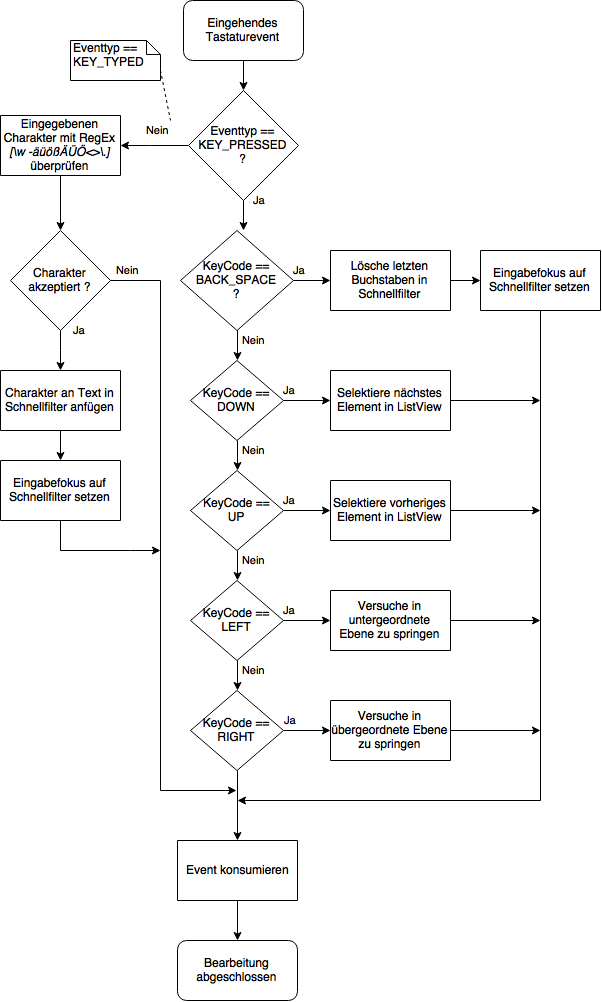
\includegraphics[width=0.75\textwidth]{grafiken/MLL_KeyCapture.png}
 \caption{Multi-Level-Liste Tastatursteuerung}
 \label{fig:mllKeyCapture}
\end{figure}
Einige Implementierungsdetails sind in dem Schaubild nicht aufgeführt, spielen aber für das grundlegende Konzept keine tragende Rolle. Wird ein Zeichen eingegeben, wird zunächst mit Hilfe eines regulären Ausdruckes gefiltert, ob das entsprechende Zeichen akzeptiert wird. Ist dies der Fall, wird das Zeichen direkt in das Textfeld des Schnellfilters eingegeben und der Fokus darauf gesetzt. Handelt es sich um einen \enquote{normalen} Tastendruck (der keinem Unicode-Charakter zugeordnet ist) wird auf Basis einer Fallunterscheidung jeweils eine zugeordnete Aktion ausgeführt.\par
Schwierigkeiten traten beim automatischen Scrolling auf, das ausgelöst werden muss, sobald die Selektion außerhalb des sichtbaren Bereiches gesetzt wird. Die nativ implementierte Scroll-Funktion ermöglicht es nur, eine bestimmte Zelle zum Anfang des \textit{ViewPorts}, also des sichtbaren Bereiches zu scrollen. Ein solches Verhalten ist ungewöhnlich und dementsprechend nicht intuitiv verwendbar. Daher muss eine weitere Berechnung durchgeführt werden, durch die erschlossen werden kann, welches Listenelement an die erste Stelle gescrollt werden muss, damit die gerade selektierte Zelle in den sichtbaren Bereich gelangt.\par
\heading{Ergebnisansichten}
Wie auch bei der mehrstufigen Liste in der Filteransicht, kann die Drag-Geste für die verschiedenen Tabellen und Listen der Ergebnisansichten über das Panning realisiert werden, das normalerweise das Scrollen auf Touch-Geräten ermöglicht. So sind nur geringfügige Eingriffe in den vorhandenen Code nötig.\par
Das Steuern der Galerie mit Drag-Aktionen ist vergleichbar mit der Implementierung im Radialmenü. Anstatt jedoch eine Winkelberechnung zwischen Start- und derzeitiger Position der Geste durchzuführen, wird nur die horizontale Änderung betrachtet und daraufhin die Verschiebung der Vorschauleiste auf der X-Achse berechnet. Auch hier werden wieder verschiedene Properties für die Berechnung der Verschiebung genutzt. So hat es den Anschein, als würde der Nutzer die Bordüre der Vorschaubilder von einer Koordinate zu einer anderen ziehen können. Mit Abschluss der Aktion wird die Position der Leiste per Animation korrigiert, sodass das Element, das dem Mittelpunkt des sichtbaren Teils der Leiste am nächsten ist, ausgewählt wird.\par
\begin{figure}[H]
 \centering
 
\includegraphics[width=0.75\textwidth]{grafiken/gallery_drag.png}
 \caption{Galerie Gestensteuerung}
 \label{fig:mllKeyCapture}
\end{figure}
Im Lesemodus wird statt einer Drag-Aktion die Umsetzung einer Swipe-Geste benötigt. Diese ist wiederum ähnlich aufgebaut wie die Drag-Aktion in der Galerie. Der Unterschied besteht darin, dass die Position der einzelnen Seiten im Lesemodus nicht konstant animiert werden muss.  Das bedeutet, eine Aktualisierung ist erst mit Abschluss der Geste erforderlich. Wird die Geste von links nach rechts ausgeführt, liegt eine positive Änderung der X-Koordinate von Start zu Zielpunkt der Geste vor. Dies resultiert in einem \enquote{Zurückblättern}, andernfalls in einem \enquote{Vorblättern}.\par
Die Unterstützung der Tastatur in den Ergebnistabellen ist konzeptionell parallel zu der Implementierung in der Multi-Level-Liste aufgebaut. Auch hier werden wieder Fallunterscheidungen für die verschiedenen akzeptierten Eingaben benötigt. Allerdings muss hier beim Wechsel der Selektion unterschieden werden, ob bei der Tabelle Zeilen- oder Zellselektion aktiviert ist. Bei Zellselektion muss zusätzlich zu dem vertikalen Scrollverhalten auch das horizontale Scrollverhalten nach dem gleichen Schema angepasst werden, damit das Konzept intuitiv verwendbar ist.\par
Die Eingabeunterstützung für die Galerie-Komponente besteht, ähnlich der Multi-Level-Liste, auch wiederum aus dem Teil, der die die \textit{KEY$\_$PRESSED}-Events behandelt und dem Teil, der die \textit{KEY$\_$TYPED}-Events behandelt. Die Fallunterscheidung der \textit{KEY$\_$PRESSED}-Events ist konsistent mit den anderen Ergebnisansichten und der Steuerung in der Filteransicht. Es werden also die Pfeiltasten (in diesem Falle $\leftarrow$- und $\rightarrow$) unterstützt, sowie die Enter-Taste zum Ausführen der assoziierten Aktion (hier: Öffnen des Lesemodus). Die Verarbeitung der Texteingabe funktioniert ein wenig anders als im Filterbildschirm. Hier führt die Eingabe eines Zeichens dazu, dass eine Zeichenkette erstellt wird. Es wird sofort innerhalb der Bezeichnungen der Modellelemente, die in der Galerie angezeigt werden, nach dem ersten Eintrag gesucht, der mit der Zeichenkette beginnt. Anfänglich besteht die Zeichenkette nur aus einem Zeichen. Wird innerhalb von 500 Millisekunden ein weiteres Zeichen getippt, wird es an die Zeichenkette angefügt und die Suche wird erneut mit der verlängerten Zeichenkette ausgeführt. So ist es möglich, auch nach längeren Bezeichnern zu suchen, wenn einige Bezeichner mit den gleichen Anfangsbuchstaben beginnen. Erzielt die Suche einen Treffer, wird die Galeriekomponente zu dem entsprechenden Element gescrollt.\par
Der Lesemodus unterstützt diese Funktion bewusst nicht, da diese Ansicht für das \enquote{Blättern} entworfen wurde, nicht um nach den Details spezieller Elemente zu suchen. Für diese Funktionalitäten stehen die anderen Ergebnispräsentationen zur Verfügung. Wie bei den anderen Ansichten ist hier das Wechseln der Datenblätter per Pfeiltasten durch eine einfache Fallunterscheidung implementiert. \par
\chapter{Adaptive Design}
Das Adaptive Design dient dazu, die Anwendung an verschiedene Bildschirmgrößen anzupassen. Da das Responsive Design eng mit den Kapazitäten des CSS3-Standards und HTML(5) als beschreibende Sprache verbunden ist, lässt sich das Konzept nicht problemlos von der Webentwicklung auf die Client-Softwareentwicklung übertragen. Zudem wäre die Implementierung eines dynamischen Rasters in dieser Phase der Entwicklung mit unverhältnismäßig hohen Aufwänden verbunden, weshalb davon abgesehen wird. Es wird daher nur mit adaptiven Methoden gearbeitet, um das gewünschte Ergebnis zu erzielen.\par
Die derzeit erforderliche Mindestauflösung der Monitore, um die Anwendung ohne Einschränkungen bedienen zu können, wurde auf 1680 x 1050 Pixel festgelegt. Dieser Wert entspricht den kleinsten Arbeitsmonitoren der derzeitigen Endanwender. Durch Tests ist aufgefallen, dass bei Monitoren mit einer kleineren Auflösung, wie z.B. Tablet-PCs, Convertibles oder ältere Beamer, einige Bedienelemente nicht mehr bedienbar sind. Sie werden außerhalb des sichtbaren Bereiches geschoben oder werden von anderen Objekten überlagert. Außerdem wird die Individualisierbarkeit der Anwendung durch die feste Größe des Fensters, die nicht unter 1680 x 1050 Pixel sinken kann, stark eingeschränkt.\par
Das Design muss an den entsprechenden Stellen so angepasst werden, dass die Größe der Anwendung variabler ist und diese auch auf Anzeigen mit geringerer Auflösung verwendet werden kann. Eine wichtige Anforderung ist, das Design in der optimalen Fenstergröße von 1680 x 1050 Pixeln (abzüglich Windows- Startleiste) nicht zu verändern.\par
\section{Analyse und Konzept} \label{sec:responsiveConcept}
Zunächst müssen die Problemstellen identifiziert werden. Für die Analyse wird die Beschränkung der Fenstergröße aufgehoben und die Anwendung in allen existierenden Ansichten verkleinert. Für die gefundenen Probleme werden Lösungen erarbeitet und später implementiert.\par
\subsection{Hauptbildschirm}
Bereits bei der Analyse der Anwendung im Startbildschirm fällt auf, dass bei horizontaler Verkleinerung des Fensters die Sidebar nicht mehr sichtbar ist. Wird die Größe in vertikaler Ausrichtung verringert, repositioniert sich die Komponente im Content-Bereich nicht korrekt und überlagert ab einer gewissen Größe die Navigationsleiste. Sowohl die Seitenleiste als auch die Navigationsleiste werden durch diese Probleme zu großen Teilen unbedienbar. Innerhalb der Navigationsleiste wurden ebenfalls Probleme gefunden. Bei verringerter horizontaler Größe, überlagern nach einiger Zeit auch der Hilfetext und das Logo die Bedienelemente der Navigationsleiste, wodurch die darunter liegenden Elemente nicht mehr angeklickt werden können.\par
\begin{figure}[H]
 \centering
 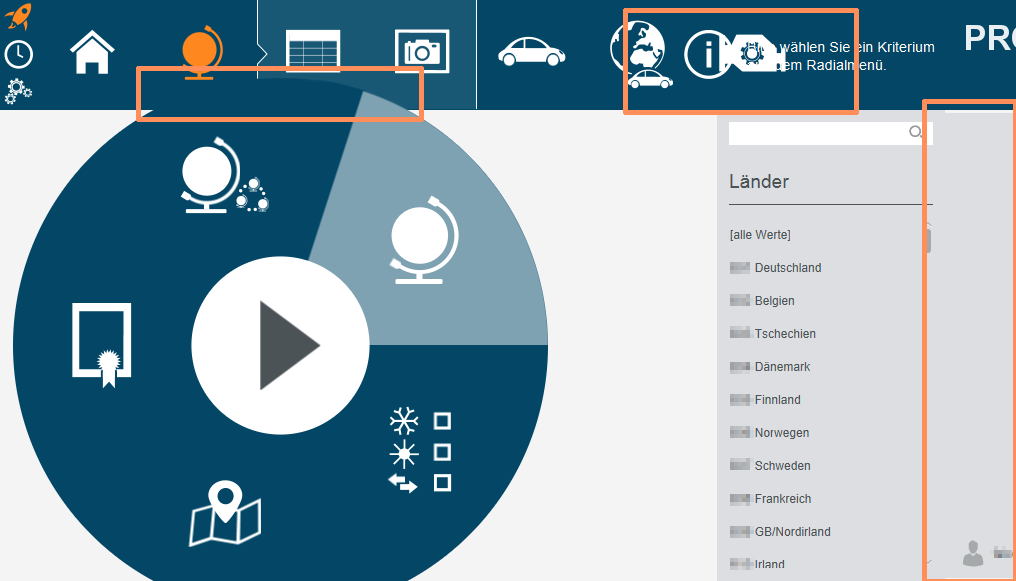
\includegraphics[width=0.6\textwidth]{grafiken/radial_bug.png}
 \caption{Layoutprobleme Hauptbildschirm}
 \label{fig:layoutMainScreen}
\end{figure}
Zur Behebung der allgemeinen Positionierungsprobleme im Hauptfenster muss das Layoutverhalten des Wurzelknotens verändert werden, sodass die Seitenleiste eine unveränderliche Position hat und diese nicht mehr durch die Position und Größe des Hauptinhaltes bestimmt wird. Die Komponenten dürfen keinesfalls außerhalb des sichtbaren Bereiches liegen. Innerhalb der Navigationsleiste kann das Problem so behoben werden, dass der Hilfetext anfänglich die Breite je nach verbleibendem Platz verringert und bei zu geringer Breite verschwindet. Bietet der Navigationsbereich wieder ausreichend Platz, erscheint der Hilfetext wieder. Als zweite Stufe wird selbiges Verfahren auf das Logo angewandt, dass bei zu geringer Größe ebenfalls Elemente verbirgt.\par
\subsection{Filterbildschirm}
Auch hier stellten sich zwei verschiedene Probleme heraus. Das erste Problem ist die Position des Radialmenüs. Dieses überlagert, sobald der vorhandene Platz nicht mehr ausreicht, die Navigationsleiste. Zudem stellt sich in dem Filter für die kombinierten Daten der Umstand ein, dass zwei Schaltflächen zum Umschalten des Radialmenüs in der linken oberen Ecke des Radialmenüs vorhanden sind. Auch diese werden durch das Radialmenü verdeckt.\par
\begin{figure}[H]
 \centering
 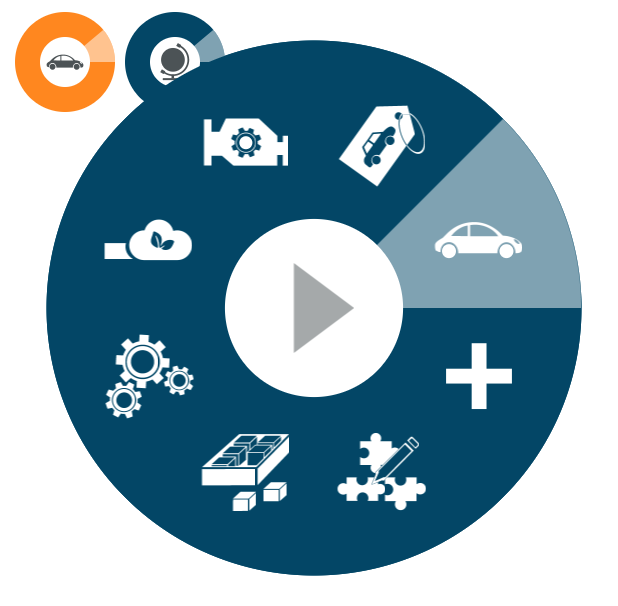
\includegraphics[width=0.4\textwidth]{grafiken/radial_bug2.png}
 \caption{Layoutprobleme Filter}
 \label{fig:layoutLtueFilter}
\end{figure}
Eine mögliche Lösung wäre, die Größe des Radialmenüs zu verringern, sobald der vorhandene Platz nicht mehr ausreicht. Dies widerspräche allerdings den Designrichtlinien, nach denen die Größe des runden Menüs exakt berechnet wurde, um im Einklang mit der Multi-Level-Liste und der Sidebar gesehen zu werden. Die andere Alternative ist es, das Verkleinern der Anwendung nur soweit zu erlauben, dass das Radialmenü noch in voller Größe (mit Abständen an allen Seiten) in dem Inhaltsbereich angezeigt werden kann. Dieser Wert liegt bei ungefähr 1024 x 768 Pixeln, was einer gängigen, jedoch geringen Monitor- oder Beamer-Auflösung entspricht.\par
Das Verkleinern der Auswahlbuttons ist ebenfalls keine Option. Durch das Begrenzen der Mindestgröße der Anwendung allerdings wird nur die rechte der beiden Schaltflächen verdeckt. Kollidieren durch das Verkleinern des Fensters das Radialmenü und besagte Schaltfläche, kann die Position des Buttons verändert werden. Er würde dann in der rechten oberen Ecke erneut auftauchen. Ist wieder ausreichend Platz vorhanden, kehrt die Schaltfläche an die ursprüngliche Position zurück. Unter normalen Umständen würde eine derartige Umsetzung nicht den Anforderungen genügen, da die Positionsänderung für leichte Verwirrung beim Anwender sorgen könnte, mangels Alternative muss die Umsetzung jedoch so erfolgen. Zudem ist sich der Nutzer bewusst, dass er bei starker Verkleinerung der Anwendung außerhalb der optimalen Benutzungsgröße arbeitet und nimmt das Risiko einer verringerten Usability im Austausch für die Individualisierbarkeit hin.\par
\subsection{Ergebnisansichten}
Bei sämtlichen Ergebnisansichten fällt auf, dass diese sich bereits an die Größe des Inhaltsbereiches anpassen. In einigen Ansichten, wie der Ergebnistabelle und der Listenansicht wirken die Informationen bei kleineren Auflösungen jedoch stark gedrängt. Der Nutzer muss viel scrollen, um in dem kleinen Bereich die Werte angezeigt zu bekommen, nach denen er im Augenblick sucht. Um dies komfortabler zu gestalten, sollte es möglich sein, die Sidebar und die Navigationsleiste übergangsweise auszublenden und so die Ergebnisansicht auf dem gesamten verfügbaren Raum präsentiert zu bekommen. Das Verlassen des Vollbildmodus kann durch einen hinzugefügten Button oder durch das Drücken der ESC-Taste erfolgen. Um zu dem Verständnis der Funktion beizutragen, erfolgt der Zustandswechsel animiert, indem die Navigationsleiste nach oben aus de Fenster fährt und die Sidebar nach rechts. Währenddessen \enquote{wächst} der Inhaltsbereich auf die gesamte Fenstergröße an.\par
\section{Umsetzung} \label{sec:responsiveImplementation}
Die Implementierung erfolgt auf Basis der Design-Entscheidungen des vorangegangenen Abschnittes.\par
\subsection{Wurzel-Komponente}
Einige der Implementierungsaufgaben lassen sich zusammenfassen und durch die Implementierung einer neuen Komponente verwirklichen. Diese Komponente wird anstelle der derzeitigen Wurzel-Komponente der Anwendung eingesetzt. Zuvor bestand diese aus einer \textit{BorderPane}, die es erlaubt, Komponenten so anzuordnen, dass diese sich an den Seitenrändern orientieren und eine weitere \textit{Center}-Bereich ausfüllt. Eine ähnliche Komponente wird auch für das neue Verhalten benötigt.\par
Durch die Erweiterung der \textit{BorderPane}-Komponente würden so die Funktionalitäten dieser übernommen und zum Teil verändert, sowie weitere hinzugefügt werden können. So würden sich die meisten Layoutprobleme bei kleinen Fenstergrößen beheben lassen und zusätzlich die Vollbild-Funktion für die Ergebnisansichten implementiert werden können.\par
Jeder JavaFX Container-Knoten implementiert eine Methode \textit{\#{}layoutChildren()}. Diese bestimmt die Position und Größe der beinhalteten Komponenten. Die Methode kann überschrieben werden, um das Standardverhalten zu ändern. Die abgeleitete \textit{BorderPane}, die den neuen Wurzelknoten darstellt, berechnet die Position der Komponenten auf eine andere Weise. So wird erreicht, dass sich die Sidebar stets am äußeren rechten Rand befindet und nicht aus dem sichtbaren Bereich verschwindet, selbst, wenn die Mindestgröße der \textit{Center}- Komponente dadurch unterschritten wird. Durch das überschriebene Layoutverhalten wird der Position und korrekten Darstellung der Elemente eine höhere Gewichtung zuteil als der festgelegten Größe. Durch jene Veränderungen an der Größen- und Positionsberechnung wird ebenfalls verhindert, dass die Navigationsleiste überlagert wird.\par
Die Vollbildfunktion ist als Teil des Layoutverhaltens implementiert. Für die Positionsberechnung der Navigationsleiste und der Seitenleiste muss in Betracht gezogen werden, ob der Vollbildmodus aktiv oder inaktiv ist. Ist er inaktiv, kann die Positionsberechnung wie gewohnt ausgeführt werden. Bei aktivem Vollbildmodus muss die Position der Navigationsleiste und die Position der Sidebar im Nachhinein modifiziert werden, sodass die \textit{Center}-Komponente das gesamte Fenster zur Verfügung hat.\par
\begin{figure}[H]
 \centering
 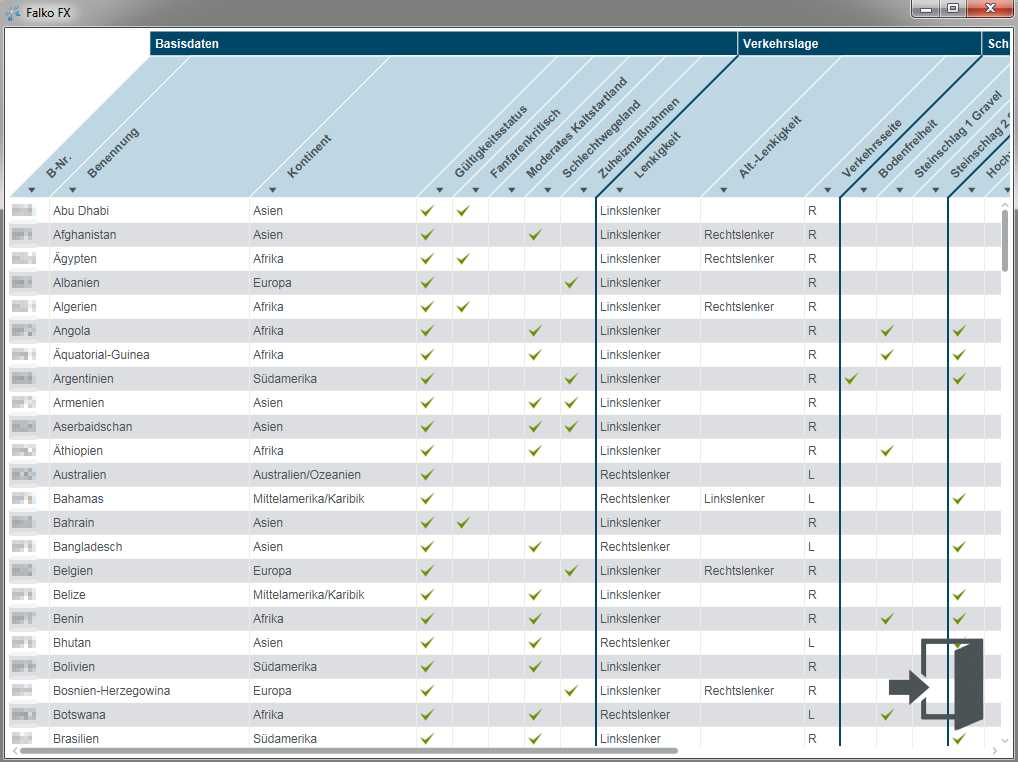
\includegraphics[width=0.6\textwidth]{grafiken/fullscreen.png}
 \caption{Vollbildmodus}
 \label{fig:fullscreenMode}
\end{figure}
Damit der Übergang vom normalen Modus in den Vollbildmodus und zurück für den Nutzer plausibel ist, wird eine Animation verwendet. Diese sorgt dafür, dass sich die äußeren Elemente aus dem Fenster bewegen, während das mittlere Element wächst. Dies geschieht, indem ein Property (\textit{Vollbildfaktor}) durch eine JavaFX-Animation verändert wird. Es ändert den Wert beim Wechsel in dem Vollbildmodus von 0 zu 1 bzw. von 1 zu 0, wenn der Modus wieder verlassen wird. Die JavaFX-Animation sorgt dafür, dass innerhalb einer gegebenen Zeitspanne (in diesem Fall 1 Sekunde) der Wert mehrfach verändert wird, bis der Zielwert erreicht ist. Ein \textit{Listener} auf dem \textit{Vollbildfaktor} sorgt dafür, dass bei jeder Aktualisierung des Wertes der Layout-Algorithmus erneut ausgeführt ist. Dieser zieht den Vollbildfaktor in Betracht und richtet die Elemente entsprechend aus.\par
Eine schematische Darstellung dieses Verfahrens ist in dem nachfolgenden Flussdiagramm festgehalten:
\begin{figure}[H]
 \centering
 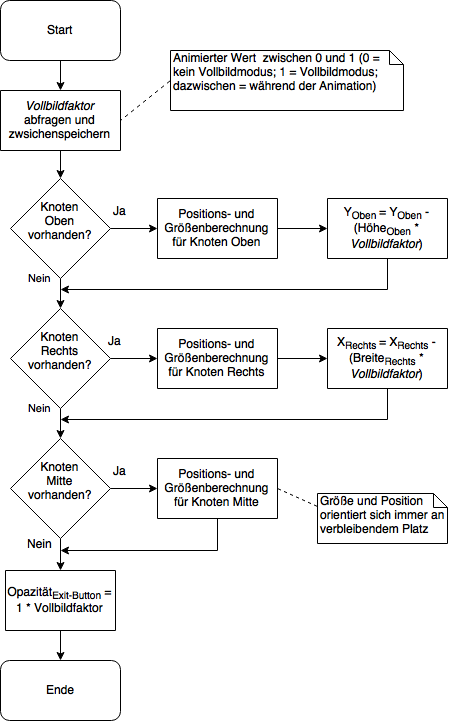
\includegraphics[width=0.75\textwidth]{grafiken/root_node_layout.png}
 \caption{Wurzelknoten Layoutverfahren}
 \label{fig:rootNodeLayout}
\end{figure}
\subsection{Navigationsleiste}
Um in der Navigationsleiste die weniger wichtigen Elemente, sprich Infotext und Logo, sukzessive zu entfernen, wird ein Listener benötigt, der an die Breiten-Property der gesamten Navigationsleiste angehängt wird. Verändert diese sich, wird eine Berechnung ausgeführt, die überprüft, ob noch genügend Platz für die einzelnen Elemente vorhanden ist. Ungeachtet der Implementierungsdetails, ist die Logik schnell erklärt:
\begin{itemize}
	\item Der Hilfetext wird angezeigt, wenn:
 		\begin{equation}
 			Breite_{Navi-leiste} >= Breite_{Navi-elemente} + Breite_{Logo} + MinBreite_{Hilfetext}
 		\end{equation}
 	\item Das Logo wird angezeigt, wenn:
 		\begin{equation}
	 		Breite_{Navi-leiste} >= Breite_{Navi-elemente} + Breite_{Logo}
 		\end{equation}
\end{itemize}
Damit das Logo bei Entfernen des Infotextes am rechten Rand der HBox, aus der die Navigationsleiste besteht, positioniert bleibt, wird ein unsichtbarer Platzhalter eingefügt, der stets die Breite des restlichen zur Verfügung stehenden Platzes einnimmt. Wird der Infotext wieder eingeblendet, wird der Platzhalter entfernt. Dies ist notwendig, da HBox-Container die Eigenschaft haben, alle beinhalteten Elemente horizontal direkt nebeneinander anzuordnen.\par
\begin{figure}[H]
 \centering
 
\includegraphics[width=0.8\textwidth]{grafiken/fix_nav.png}
 \caption{Schmale Navigationsleiste ohne Infotext}
 \label{fig:fixNav}
\end{figure}
\subsection{Filterbildschirm}
%\editHere{BLA}\par
Um den Button im Filterbildschirm repositionieren zu können, wird berechnet, ob das Radialmenü mit dem rechten der Auswahlbuttons kollidiert. Der Kollisionsalgorithmus nutzt die Radien der beiden betrachteten kreisförmigen Elemente (rechter Button und Radialmenü), um zu determinieren, ob die rechte der Schaltflächen die Position wechseln muss. Abhängig von der Breite und Höhe des Fensters wird dieser Wert aktualisiert. Tritt eine Kollision ein, muss der Button die Position ändern. Der Button erhält seine Ausgangsposition zurück, wenn die Berechnung von dem ursprünglichen Mittelpunkt und dem Radius der Schaltfläche eine Kollision ausschließt.\par
\begin{figure}[H]
 \centering
 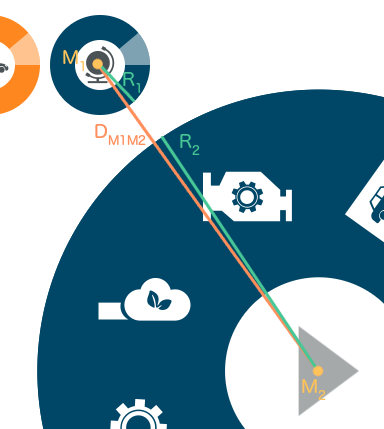
\includegraphics[width=0.4\textwidth]{grafiken/radius.png}
 \caption{Kollisionsberechnung im Filterbildschirm}
 \label{fig:collisionFilter}
\end{figure}
Eine Kollision liegt vor, wenn:\par
\begin{equation}
	D_{M1M2} <= R_1 + R_2 + Padding
\end{equation}
Das Padding bezeichnet den Mindestabstand zwischen den beiden Objekten. Liegt dieser bei 0, ist eine Kollision erst bei direktem Kontakt der Objekte gegeben.\par
Wird eine Kollision erkannt, wechselt der Button die Position auf die rechte Seite des Radialmenüs:
\begin{figure}[H]
 \centering
 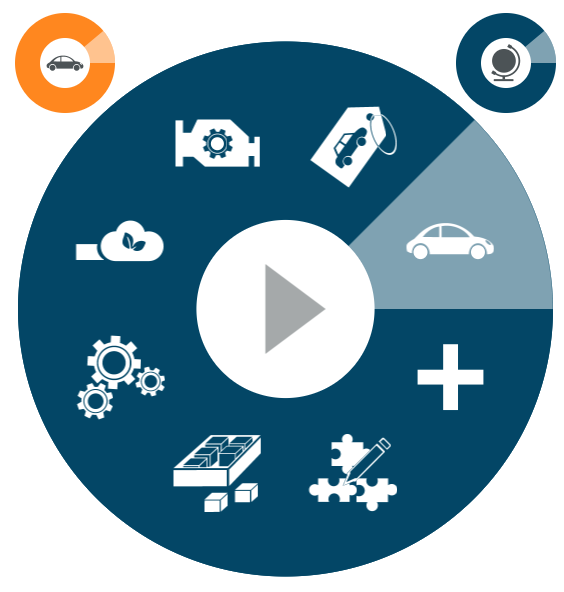
\includegraphics[width=0.5\textwidth]{grafiken/fix_filter.png}
 \caption{Alternative Buttonposition im Filterbildschirm}
 \label{fig:fixFilter}
\end{figure}
\chapter{Analysen und Nutzertests}
\section{Entwicklung des Analyse-/Testkonzepts} \label{sec:analysisConcept}

\section{Durchführung der Analysen} \label{sec:analysisExecution}

\section{Durchführung der Nutzertests} \label{sec:testExecution}

\section{Auswertung der Ergebnisse} \label{sec:analysisConclusion}
\chapter{Optimierung auf Basis der ausgewerteten Testdaten}
Für die in Kapitel \ref{sec:analysisTests} aufgedeckten Probleme werden in diesem Abschnitt Lösungen erarbeitet und umgesetzt. Abschließend wird ein vergleichender Kontrolltest durchgeführt, um zu verifizieren, ob die unternommenen Veränderungen wirklich den gewünschten Effekt auf den Nutzer haben.\par
\section{Design der Lösungen} \label{sec:optiDesign}
Das erste zu behandelnde Problem ist die die Filterauswahl in der Sidebar. Hier muss verdeutlicht werden, dass die Elemente angeklickt werden können und sowohl das \textbf{-} -Icon, das nur als Hover-Effekt angezeigt wird, als auch der Text zu einer Einheit gehören. %Zwar unterstützt die orangefarbene Hinterlegung des gesamten Elementes während des Hoverns bei der Identifizierung als ein einzelnes Objekt, aber die Animation, mit der das \textbf{-} -Symbol erscheint, wirkt dem entgegen (Gesetz des gemeinsamen Schicksals).
Eine einfache Möglichkeit, zu signalisieren, dass das gesamte Element angeklickt werden kann, ist das Hinzufügen des Hand-Cursors für alle Elemente, die angeklickt werden können.\par
%Für den Kopfzeilenfilter der Ergebnistabelle kann eine ähnliche Suchfunktion umgesetzt werden, wie für die Galerie. Eine Freitexteingabe, die ein Scrollen zum gesuchten Element hervorruft, kann hier genauso dabei unterstützen, das richtige Element zu finden. Das gleiche Konzept kann auch für die Ergebnistabelle selbst übernommen werden. In diesem Fall würde das primäre Attribut, die Benennung, für die Suche ausschlaggebend sein.\par
Während der Lesemodus aktiv war, versuchte ein Nutzer die Galerie im Hintergrund zu bedienen. Um dies zu unterbinden und deutlich zu machen, dass die Bedienelemente im Hintergrund derzeit nicht verwendbar sind, kann entweder die Transparenz des vordergründigen Lesemodus verringert werden oder alternativ über die hintergründigen Komponenten ein Effekt gelegt werden, der die Darstellung \enquote{verwischt}. Dieser Effekt nennt sich \textit{Blur}-Effekt. Dadurch sind die Elemente noch immer sichtbar, aber durch die verschwommenen Konturen wird deutlich, dass sie derzeit nicht für eine Bedienung geeignet sind. Aufgrund der Ästhetik ist die zweite Variante die bevorzugte Alternative.\par
Das \ding{58}-Icon in der Navigationsleiste bereitete Probleme bei der Bedienung, da es nicht als klickbares Element wahrgenommen wurde. Um die Komplikation zu beheben, muss die Aufmerksamkeit des Benutzers bewusst auf das neu erschienene Element gelenkt werden. Dies kann durch eine Animation geschehen, die abläuft, sobald das Symbol angezeigt wird. Ein \textit{Glow}-Effekt (kurzes Aufblinken) sollte diesen Zweck erfüllen.\par
Der Eintrag \textit{[Alle Werte]} in der Multi-Level-Liste sollte sich, gemäß des Gesetzes der Prägnanz, deutlicher von dem Rest der Einträge abheben, damit es eher erkannt und nicht als Teil der möglichen Werte gesehen wird. Ein einfaches Fettdrucken des Textes sollte für diesen Zweck genügen. Außerdem kann der Eintrag entfernt werden, sobald kein weiteres Element in der Liste ist und einem Infotext weichen, durch den die leere Liste erklärt wird.\par
Für den Vollbildmodus kann der Hotkey \enquote{F11} bedenkenlos hinzugefügt werden. Dies muss jedoch auf andere Weise geschehen als mit dem bisherigen Mnemonic-Konzept, das bewusst nur sichtbare Elemente unterstützt. Die Vollbildfunktion ist nicht immer sichtbar.\par
Sämtliche Ergebnistabellen und -listen benötigen einen Hinweistext, der angezeigt wird, wenn kein Element in diesen dargestellt wird, um dem Punkt \textit{\enquote{Gibt es Unterstützung bei Fehlern?}} der Usability-Heuristik von Nielsen und Molich zu entsprechen.\par
Die Subnavigation in der Detailansicht ist für den Anwender nicht eindeutig erkennbar. Unter Umständen Ist der orangefarbene Text des selektierten Unterpunktes schwerer zu erkennen als das schwarz des nicht-selektierten Unterpunktes. Ein kurzer Blick zu diesen Elementen reicht nicht aus, um den selektierten Punkt auszumachen, daher sollte der Text durch Fettdrucken prägnanter dargestellt werden.\par
% Hilfetexte?
\section{Umsetzung} \label{sec:optiImplementation}
\heading{Mauszeiger Filterauswahl}
Der Mauszeiger auf den einzelnen Elementen der Filterselektion ließ sich umsetzen, indem der Cursor innerhalb der \textit{\#{}updateItem}-Methode der verwendeten Listenzelle gesetzt wird. Hierbei muss darauf geachtet werden, dass der Cursor gesetzt wird, wenn die Listenzelle einen Text beinhaltet und zurückgesetzt wird, falls der Text leer ist. Die Besonderheit der Listenzelle in JavaFX ist die Wiederverwendung dieser. Anstatt für jedes Item der Liste eine neue Listenzelle zu erzeugen, werden die Zellenobjekte wiederverwendet und nur die Eigenschaften und der Inhalt dieser aktualisiert.\par
\heading{Lesemodus}
Um den Blur-Effekt für den Hintergrund des Lesemodus zu setzen, wird die Methode \textit{\#{}setEffect} verwendet, die auf jeder JavaFX-Komponente verfügbar ist. Als Übergabeparameter dient ein sogenanter BoxBlur-Effekt, der vorab konfiguriert wird. Wird der Effekt auf dem Wurzelknoten des ursprünglichen Inhaltes gesetzt, der mit Öffnen des Lesemodus in der Hintergrund rückt, wird die Ansicht des Hintergrundes verschwommen und der Fokus auf die vordergründigen Objekte gelenkt. Die Wahrscheinlichkeit, dass ein Anwender versucht, Bedienelemente zu nutzen, die sich im Hintergrund befinden, wird dadurch stark verringert. Ein weiterer Vorteil des Effektes ist, dass so die Illusion von Tiefenunschärfe erzeugt wird, wodurch die dreidimensionale Darstellung der verschiedenen Ebenen (Lesemodus und Hintergrund) verstärkt wird.\par
\begin{figure}[H] 
	\centering
	\subfloat[Ohne Blur] {
		 
\includegraphics[width=0.45\textwidth]{grafiken/readmode_no_blur.png}
	}
	\hspace{1.0em}
	\subfloat[Mit Blur] {
		 
\includegraphics[width=0.45\textwidth]{grafiken/readmode_blur.png}
	}
	\caption{Beispiel: Blur-Effekt im Lesemodus}
	\label{fig:blurGallery}
\end{figure}
\heading{Erweiterte Funktionen der Navigationsleiste}
Auch für das Hervorheben des \ding{58}-Icons in der Navigationsleiste kommt ein Effekt zum Tragen. Allerdings wird hier ein sogenannter \textit{DropShadow} verwendet. Die Eigenschaften des Effektes sind so konfiguriert, dass der \textit{DropShadow} standardmäßig nicht sichtbar ist, da die Größe 0 x 0 Pixel beträgt. Wird zu einem anderen Menüpunkt gesprungen, der erweiterte Funktionen unterstützt, wird mit Erscheinen des \ding{58}-Icons der Effekt im Rahmen einer Animation so verändert, dass sich die Größe von anfänglich 0 Pixeln gleichmäßig in alle Richtungen vergrößert. Die Animation ist so eingestellt, dass sich der Effekt 1 Sekunde lang ausbreitet und mit Abschluss dieser innerhalb einer weiteren Sekunde wieder zusammenzieht. Das Zusammenziehen wird allerdings durch das Animieren eines anderen Properties gelöst. Der \textit{DropShadow} besitzt ein \textit{Spread}- Property, das die Ausbreitung des Effektes bestimmt. Sobald dieser Wert 0 erreicht, ist die Animation abgeschlossen und alle Werte werden auf ihren Ausgangszustand zurückgesetzt. Durch das Animieren der beiden unterschiedlichen Effekt-Eigenschaften wird die Aufmerksamkeit des Anwenders auf attraktive Weise auf das neu erschienene Symbol gelenkt.\par
\begin{figure}[H]
 \centering
 
\includegraphics[width=0.75\textwidth]{grafiken/glow_animation.png}
 \caption{Glow Animation}
 \label{fig:glowAnimation}
\end{figure}
\heading{Spezialeintrag \textit{[Alle Werte]}}
Das Fettdrucken des Eintrages \textit{[Alle Werte]} in der Multi-Level-Liste konnte durch eine simple Fallunterscheidung innerhalb der angepassten Listenzellen-Klasse gelöst werden. Bei Ausführung der \textit{\#{}updateItem}-Funktion wird überprüft, ob das Element, das ab in der Listenzelle angezeigt werden soll in der Werteliste enthalten ist, die der JavaFX-ListView zugrunde liegt. Ist dies nicht der Fall, handelt es sich um das nachträglich hinzugefügte Spezialelement \textit{[Alle Werte]}. In diesem Falle wird der Listenzelle eine CSS-Klasse zugewiesen, durch die jeglicher in der Zelle enthaltener Text fett dargestellt wird. Das Element grenzt sich so deutlich von den übrigen Elementen ab.\par
\begin{figure}[H]
 \centering
 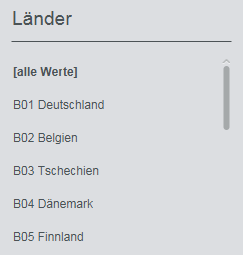
\includegraphics[width=0.35\textwidth]{grafiken/mll_Werte.png}
 \caption{Multi-Level-Liste Spezialeintrag}
 \label{fig:mllSpecialValue}
\end{figure}
\heading{Schnelltaste für Vollbildmodus}
Das Aktivieren des Lesemodus ist nun auch per Schnelltaste \textit{F11} möglich. Dazu wird die Tastatureingabe über das bereits vorgestellte Konzept der globalen Eingabeerkennung (vgl. Kap. \ref{sec:interactionImplementation}) verarbeitet. Der Vollbildmodus wird nur aktiviert, wenn der korrespondierende Menüpunkt auch aktiviert ist und die gedrückte Taste der \textit{F11} Taste entspricht. In diesem Fall wird das Event konsumiert - andere, im Szenegraphen tiefer liegende Knoten, die ein solches Event ggf. behandeln würden, werden in diesem Falle nicht von dem Event benachrichtigt.\par
\heading{Hilfetext leere Liste/ Tabelle}
Der Hilfetext für leere Tabellen und Listen wird durch ein Label repräsentiert, dessen Sichtbarkeit von der Länge der jeweiligen Liste oder Tabelle abhängt. Sobald kein Element mehr vorhanden ist, wird das Label sichtbar. Der Text liegt also immer über der entsprechenden Ansicht, wird jedoch nur in dieser speziellen Situation angezeigt. Die Position des Textes entspricht der eigentlichen Position der ersten Zeile. In der Multi-Level-Liste wird zudem der Spezialeintrag \textit{[Alle Werte]} entfernt, wenn der Hilfetext dargestellt werden soll.\par
\begin{figure}[H]
 \centering
 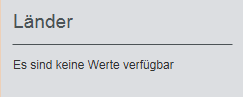
\includegraphics[width=0.35\textwidth]{grafiken/mll_no_values.png}
 \caption{Multi-Level-Liste Infotext}
 \label{fig:mllNoValues}
\end{figure}
\heading{Subnavigation Detailansicht}
Damit das ausgewählte Element in der Subnavigation der Detailansicht deutlicher hervorgehoben wird, wird der Text fett gedruckt. Die Funktion wird über eine CSS-Pseudoklasse realisiert, die auf dem Label des selektierten Elementes gesetzt und bei Änderung aktualisiert wird. Eine CSS-Pseudoklasse wird in einer CSS-Datei durch einen Bezeichner angesprochen, der durch einen Doppelpunkt vom Rest des CSS-Selektors abgetrennt wird. Die für das Label neu definierte Pseudoklasse namens \enquote{selected} wird immer dem Punkt zugewiesen, der gerade angewählt ist. Der CSS-Selektor trifft also immer auf das Label zu, das den \enquote{selektiert}-Status besitzt und stellt dessen Text hervorgehoben dar.\par
\begin{figure}[H]
 \centering
 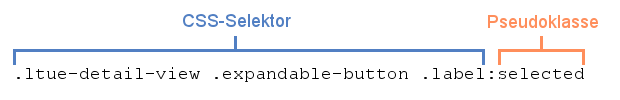
\includegraphics[width=0.9\textwidth]{grafiken/pseudoklasse.png}
 \caption{CSS Pseudoklasse}
 \label{fig:cssPseudoclass}
\end{figure}
Eine Pseudoklasse wird in JavaFX durch eine Ableitung der abstrakten Klasse \textit{Pseudoclass} ermöglicht. Die einzige Information, die durch diese Ableitung zur Verfügung gestellt wird, ist der Name der Pseudoklasse. Durch den Aufruf \textit{Node\#{}pseudoClassStateChanged(Pseudoclass, boolean)} kann der Status der Pseudoklasse verändert werden. Die Pseudoklasse muss der Komponente dazu nicht explizit hinzugefügt werden.\par
\begin{figure}[H]
 \centering
 
\includegraphics[width=0.5\textwidth]{grafiken/detailPage_bold.png}
 \caption{Detailansicht Überschrift}
 \label{fig:detailPageBold}
\end{figure}
\section{Vereinfachte Kontrolltests} \label{sec:optiQuality}
Zur Verifikation, dass die auf Basis der Nutzertests umgesetzten Funktionen eingänglich sind und tatsächlich eine Optimierung darstellen, wird ein vereinfachter, formloser A/B-Test durchgeführt. Im Rahmen des Testes werden die Funktionen in ihrer bisherigen Form und in ihrer Form nach der Implementierung durch einige Testkandidaten verglichen. Die Kandidaten müssen sich jeweils für die von ihnen bevorzugte Lösung entscheiden. Der Vergleich kann nur bei Funktionen durchgeführt werden, die eine Änderung am User-Interface erforderlich machten. Die Kandidaten sind zum Teil diejenigen, die auch an dem Formalen Usability-Test teilgenommen haben, als auch unbefangene Testpersonen. Insgesamt werden 6 Personen befragt.\par
\heading{Blur-Effekt im Lesemodus}
Der Effekt auf dem Hintergrund des Lesemodus wird von fast allen Kandidaten als positiv empfunden, da der Fokus auf diese Weise eher auf die vordergründigen Objekte gelenkt wird. Das Ziel der Verbesserung, den Hintergrund nicht mehr als bedienbar erscheinen zu lassen, wurde erreicht.
\heading{Erweiterte Funktionen der Navigationsleiste}
Nach Meinung der befragten Personen ist die Animation ansehnlich und trägt dazu bei, die Aufmerksamkeit auf das \ding{58}-Symbol zu lenken. Es wurden allerdings Bedenken geäußert, dass die Animation unter Umständen nicht deutlich genug sein könnte. Eine auffälligere Animation würde von erfahrenen Nutzern jedoch möglicherweise als störend empfunden werden.\par
\heading{Hilfetexte leere Tabelle/ Liste}
Die Hilfetexte bei leeren Tabellen oder Listen wurden ausnahmslos als vorteilhafte Neuerung empfunden.
\heading{Spezialeintrag \textit{[Alle Werte]}}
Bei der Funktion \textit{[Alle Werte]} in der Multi-Level-Liste gab es mehr Diskrepanz als bei den anderen umgesetzten Funktionen. Hier sind nur zwei Drittel der Befragten davon überzeugt, dass die Hervorhebung notwendig ist. Das verbleibende Drittel ist der Meinung, dass alleine durch den Text und die umschließenden viereckigen Klammern ausreichend Unterschied zu den übrigen Einträgen geschaffen wird. Obwohl die Notwendigkeit der Hervorhebung durch einige Testkandidaten angezweifelt wird, wird die Funktion nicht als nachteilig empfunden.\par
\heading{Subnavigation Detailansicht}
Auch hier waren sich die Testkandidaten uneinig, ob es nötig ist, den selektierten Punkt fettgedruckt darzustellen. 4 der 6 Personen jedoch bevorzugten die fettgedruckte Variante. Die Begründung lautete, dass ansonsten der schwarzfarbige, nicht selektierte Menüpunkt auf dem hell-orangefarbenen Hintergrund deutlicher hervorsteche als der dunkel-orangefarbene Text.\par
\chapter{Ausblick und Fazit}


\nocite{*}
\bibliography{biblio/biblio}
\listoffigures
%\listoftables

\newpage
\setglossarystyle{indexgroup}
\printglossaries

\appendix
%\chapter{Tests}
\section{Aufgabenstellungen}
\subsection{Expertentests} \label{sec:tasksExpert}
Aufgabe 1
\begin{itemize}
	\item Welche Länder werden als \enquote{Höhenland} eingestuft?
\end{itemize}
Aufgabe 2
\begin{itemize}
	\item Zeige die Datenübersicht von Deutschland an.
	\item Exportiere diese als PDF
\end{itemize}
Aufgabe 3
\begin{itemize}
	\item Welche Motoren werden in der Fahrzeugreihe \enquote{R8} der Marke \enquote{Audi} verbaut?
\end{itemize}
Aufgabe 4
\begin{itemize}
	\item Exportiere eine Excel-Übersicht über alle Fahrzeugmodelle der Marke \enquote{Porsche}, die einen \enquote{4.0L V8} Motor verbaut haben.
\end{itemize}
Aufgabe 5
\begin{itemize}
	\item Für welche Modelle des Fahrzeuges \enquote{Touran} der Marke \enquote{Volkswagen} existieren Freigaben sowohl in Deutschland, als auch in Österreich?
	\item Welche Abgaskonzepte liegen den Modellen zugrunde?
	\item Zeige nur die Abgaskonzepte an (Blende alle anderen Informationen aus).
	\item Setze die Ansicht auf den Ursprungszustand zurück.
\end{itemize}
Aufgabe 6
\begin{itemize}
	\item In welchen Ländern existiert eine Freigabe für das Modell mit der Fahrzeugbezeichnung \enquote{VW216/0EU\_{}K T-Cross} und der Abgas-Prüfnummer (Abgas PrNr) \enquote{7GM}?
	\item Betrachte die Details einer Freigabe des Modells.
\end{itemize}
Aufgabe 7
\begin{itemize}
	\item Welche Modelle des Fahrzeuges \enquote{S1} der Marke \enquote{Audi} haben eine Motorfreigabe für Deutschland.
\end{itemize}
\subsection{Nutzertests} \label{tasksUser}
Aufgabe 1
\begin{itemize}
	\item Welche Länder werden als \enquote{Höhenland} eingestuft?
\end{itemize}
Aufgabe 2
\begin{itemize}
	\item Zeige die Datenübersicht von Deutschland an. Benutze dafür keinen Filter.
	\item Exportiere diese als PDF.
	\item Wechsle zu Kanada.
	\item Vergrößere die Ansicht (Lesemodus).
\end{itemize}
Aufgabe 3
\begin{itemize}
	\item Welche Motoren werden in der Fahrzeugreihe \enquote{R8} der Marke \enquote{Audi} verbaut?
	\item Exportiere eine Excel-Übersicht über alle \enquote{R8}-Modelle. Die Übersicht soll die Fahrzeug-, Motor-, und Getriebedaten enthalten.
\end{itemize}
Aufgabe 4
\begin{itemize}
	\item Für welche Modelle des Fahrzeuges \enquote{Touran} der Marke \enquote{Volkswagen} existieren Freigaben in dem Länderverbund \enquote{EU 28}?
	\item Blende alle Informationen außer des Abgaskonzeptes aus.
	\item Öffne eine Freigabe und zeige dort die Motorfreigabe an.
	\item Kehre zur Ergebnispräsentation zurück und lasse dir die Informationen im \enquote{Vollbildmodus} anzeigen (Blende Seitenleiste und Navigationsleiste aus). 
\end{itemize}
Aufgabe 5
\begin{itemize}
	\item Zeige alle Motorfreigaben der Fahrzeugreihe \enquote{S1} in Deutschland an.
\end{itemize}
Aufgabe 6
\begin{itemize}
	\item Setze alle Einstellungen und geladenen Daten zurück.
\end{itemize}
\subsection{Usability-Befragung} \label{sec:usabilitySurvey}
Die Kurzform des AttrakDiff-Fragebogens sieht die folgenden 10 Fragen vor:
\begin{figure}[H]
 \centering
 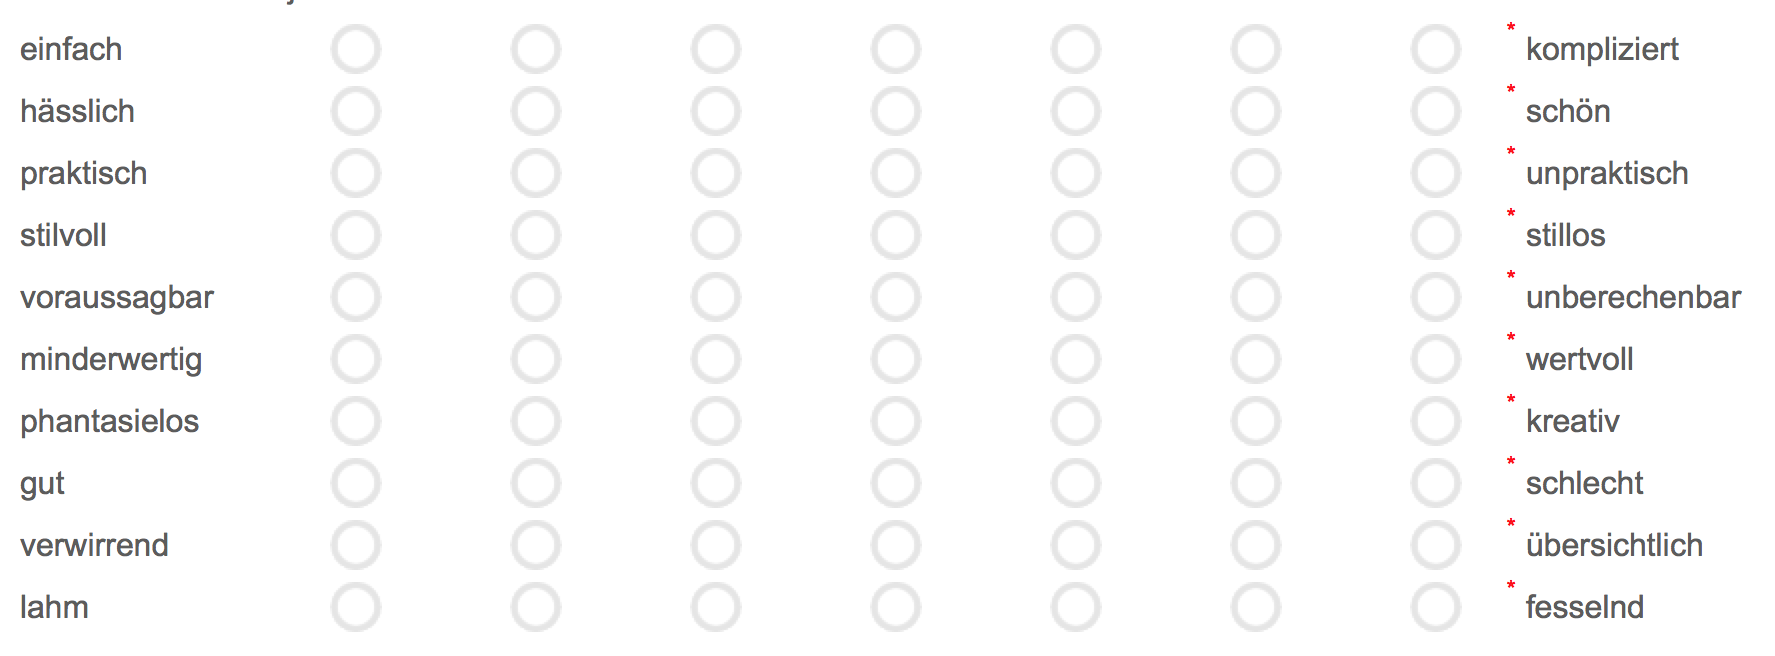
\includegraphics[width=1\textwidth]{grafiken/attrak_diff_short.png}
 \caption{AttrakDiff-Fragebogen}
 \label{fig:attrakDiffFragebogen}
\end{figure}
\section{Ergebnisse}
\subsection{Expertentest} \label{sec:resultExpert}
Es werden hier nur die Prinzipien der Heuristiken von Nielsen und Molich aufgeführt und begründet, die während der Auswertung nicht vollständig erfüllt wurden.\par
\heading{Aufgabe 1: Welche Länder werden als Höhenland eingestuft?}
% Wie Daten darstellen?
\textit{Schritt 1:} Auswählen des Anwendungsfalles \enquote{Land}\par
\textit{Schritt 2:} Auswählen des Attributes \enquote{Höhenland} für die Filterung\par
\begin{itemize}
 \item \textit{Ist die Lösung konsistent und hält Standards ein?} Standards werden eingehalten. Im Gegensatz zu der Navigationsleiste sind hier keine Tooltips für die Piktogramme vorhanden.
 \item \textit{Wird Erkennen Erinnern vorgezogen?} Die auswählbaren Kategorien sind mit sprechenden Piktogrammen versehen. Dennoch wären Tooltips von Vorteil für die korrekte Identifikation dieser.
\end{itemize}
\textit{Schritt 3:} Öffnen der Ergebnisansicht\par
\heading{Aufgabe 2a: Zeige die Datenübersicht von Deutschland an}\par
\textit{Schritt 1:} Auswählen des Anwendungsfalles \enquote{Land}\par
\textit{Schritt 2:} Auswählen des Attributes \enquote{Länderbenennung: Deutschland} für die Filterung\par
\textit{Schritt 3:} Öffnen der alternativen Ergebnisansicht (Galerie)\par
\heading{Aufgabe 2b: Exportiere diese als PDF}\par
\textit{Schritt 3:} Auswählen des Eintrages aus dem Navigation-Zusatzmenü (\ding{58}-Icon)\par
\begin{itemize}
 \item \textit{Wird Erkennen Erinnern vorgezogen?} Das \ding{58}-Icon taucht nach Wechsel in die Ergebnisansicht unter dem entsprechenden Element auf. Diese Änderung an einem normalerweise statischen Element wird u.U. durch den Benutzer nicht wahrgenommen.\par
\end{itemize}
\heading{Aufgabe 3: Welche Motoren werden in der Fahrzeugreihe \enquote{R8} der Marke \enquote{Audi} verbaut?}\par
\textit{Schritt 1:} Auswählen des Anwendungsfalles \enquote{Fahrzeug}\par
\textit{Schritt 2:} Filtern der Multi-Level-Liste nach der Bezeichnung \enquote{R8}\par
\textit{Schritt 3:} Alle Einträge auswählen\par
\begin{itemize}
 \item \textit{Wird versucht Fehler zu vermeiden?} Der Eintrag \textit{[alle Werte]} ist sichtbar, selbst wenn die Liste kein weiteres Element enthält. Dies kann den Nutzer schnell verwirren.\par
 \item \textit{Gibt es Unterstützung bei Fehlern?} Wenn es für den gewählten Schnellfiltertext keine Ergebnisse gibt, wird nur der Eintrag \textit{[Alle Werte angezeigt]}. Eine Hilfestellung zur Anzeige, dass keine Ergebnisse für den Schnellfiltertext gefunden wurden, wäre hilfreich.\par
\end{itemize}
\textit{Schritt 4:} Öffnen der Ergebnisansicht\par
\heading{Aufgabe 4: Welche Motoren werden in der Fahrzeugreihe \enquote{R8} der Marke \enquote{Audi} verbaut?}\par
\textit{Schritt 1:} Auswählen des Anwendungsfalles \enquote{Fahrzeug}\par
\textit{Schritt 2:} Auswählen der Marke Audi\par
\textit{Schritt 3:} Filtern der Multi-Level-Liste nach dem Motor \enquote{4,0L V8}\par
\textit{Schritt 4:} Auswählen aller gefundenen Einträge\par
\textit{Schritt 5:} Öffnen der Ergebnisansicht\par
\textit{Schritt 6:} Daten über \ding{58}-Menü der Navigationsleiste exportieren\par
\heading{Aufgabe 5a: Für welche Modelle des Fahrzeuges \enquote{Touran} der Marke \enquote{Volkswagen} existieren Freigaben sowohl in Deutschland, als auch in Österreich?}\par
\textit{Schritt 1:} Auswählen des Anwendungsfalles \enquote{LTÜ}\par
\textit{Schritt 2:} Auswählen des Fahrzeuges \enquote{Touran}\par
\textit{Schritt 3:} Wechsel zum Länder-Filter\par
\textit{Schritt 4:} Auswählen der Länder Deutschland und Österreich\par
\textit{Schritt 5:} Öffnen der alternativen Ergebnisansicht (Ergebnistabelle)\par
\heading{Aufgabe 5b: Welche Abgaskonzepte liegen den Modellen zugrunde?}\par
\textit{Schritt 1:} Abgaskonzept über Seitenleiste einblenden\par
\heading{Aufgabe 5c: Zeige nur die Abgaskonzepte an (Blende alle anderen Informationen aus).}\par
\textit{Schritt 1:} Abwählen aller Kategorien außer Abgaskonzept über Seitenleiste\par
\heading{Aufgabe 5d: Setze die Ansicht auf den Ursprungszustand zurück.}\par
\textit{Schritt 1:} Navigationsleiste auf Einstellungsmenü umschalten\par
\begin{itemize}
 \item \textit{Hat der Nutzer genügend Kontrolle und Freiheit?} Die Hauptnavigation ist vollständig ausgeblendet, damit die Einstellungsoptionen angezeigt werden können\par
 \item \textit{Sind Hilfe und Dokumentation vorhanden?} Es ist keine Hilfe für diese sekundären Funktionen verfügbar\par
\end{itemize}
\textit{Schritt 2:} Betätigen der \enquote{Ergebniskonfiguration zurücksetzen}- Schaltfläche\par
\heading{Aufgabe 6a: In welchen Ländern existiert eine Freigabe für das Modell mit der Fahrzeugbezeichnung \enquote{VW216/0EU\_{}K T-Cross} und der Abgas-Prüfnummer (Abgas PrNr) \enquote{7GM}}\par
\textit{Schritt 1:} Auswählen des Anwendungsfalles \enquote{LTÜ}\par
\textit{Schritt 2:} Auswählen des Fahrzeuges mit der Bezeichnung \enquote{VW216/0EU\_{}K T-Cross} für die Filterung\par
\textit{Schritt 3:} Öffnen der Ergebnisansicht (Listenansicht)\par
\begin{itemize}
 \item \textit{Gibt es Unterstützung bei Fehlern?} Wenn kein Fahrzeug selektiert ist oder keine Freigabe für das ausgewählte Fahrzeug existiert, wird die rechte Tabelle leer angezeigt. Hinweise wären hier für den Benutzer hilfreich.\par
 \item \textit{Sind Hilfe und Dokumentation vorhanden?} Der Hilfetext ist allgemeingültig gehalten und unterstützt nicht bei der Verwendung dieser speziellen Ergebnisansicht\par
\end{itemize}
\textit{Schritt 4:} Einblenden der Kategorie \enquote{Abgas} über die Seitenleiste\par
\textit{Schritt 5:} Filter in Kopfzeile der Spalte Abgas-Prüfnummer öffnen, alles deselektieren außer Wert \enquote{7GM}\par
\begin{itemize}
 \item \textit{Gibt es Unterstützung bei Fehlern?} Werden alle Einträge im Filter deselektiert, wird eine leere Tabelle angezeigt. Ein Hinweis für den Benutzer wäre hier hilfreich.\par
 \item \textit{Sind Hilfe und Dokumentation vorhanden?} Der Hilfetext gibt keinen Aufschluss über die Funktion des Filters in den Spaltenköpfen.\par
\end{itemize}
\textit{Schritt 6:} Verbleibendes Fahrzeugmodell selektieren \par
\heading{Aufgabe 6b: Betrachte die Details einer Freigabe des Modells.}\par
\textit{Schritt 1:} Doppelklick auf eine der angezeigten Länderfreigaben\par
\heading{Aufgabe 7: Welche Modelle des Fahrzeuges \enquote{S1} der Marke \enquote{Audi} haben eine Motorfreigabe für Deutschland.}\par
\textit{Schritt 1:} Auswählen des Anwendungsfalles \enquote{LTÜ}\par
\textit{Schritt 2:} Auswählen der Marke \enquote{Audi}\par
\textit{Schritt 3:} Filterung der Fahrzeuge nach der Bezeichnung \enquote{S1}\par
\textit{Schritt 4:} Auswählen aller Werte\par
\textit{Schritt 5:} Wechsel zu Länder-Filter\par
\textit{Schritt 6:} Auswählen der Länderbezeichnung Deutschland\par
\textit{Schritt 7:} Öffnen der alternativen Ergebnisansicht (Ergebnistabelle)\par
\subsection{Nutzertests} \label{sec:resultUser}
Es werden nur die gefundenen Probleme aufgeführt, die Nutzer bei der Bedienung hatten.
\heading{Aufgabe 1: Welche Länder werden als Höhenland eingestuft?}
\begin{itemize}
 \item Versucht, genau das \textbf{-} -Symbol beim Deselektieren von Filterkriterien zu treffen
 \item Gewählte Filterkriterien in Seitenleiste nicht als klickbar erkannt (zwecks Deselektierung)
 \item Versucht, über Texteingabe im Kopfzeilenfilter der Ergebnisansicht zu scrollen
\end{itemize}
\heading{Aufgabe 2: Zeige die Datenübersicht von Deutschland an.}
\begin{itemize}
 \item Versucht, die Galerie im Hintergrund zu bedienen, nachdem der Lesemodus versehentlich geöffnet wurde
 \item Das \ding{58}-Icon in der Navigationsleiste ist schwierig zu treffen, oft das Menüitem selbst angeklickt
 \item \ding{58}-Icon oft nicht wahrgenommen
 \item Scrollen in Tabelle über Tippen des Namens versucht (wie bereits in Galerie implementiert)
\end{itemize}
\heading{Aufgabe 3: Welche Motoren werden in der Fahrzeugreihe \enquote{R8} der Marke \enquote{Audi} verbaut?}
\begin{itemize}
 \item Eintrag \textit{[Alle Werte]} nicht wahrgenommen
 \item Versucht, in der Multi-Level-Liste mehrere Einträge per Shift zu selektieren
\end{itemize}
\heading{Aufgabe 4: Exportiere eine Excel-Übersicht über alle Fahrzeugmodelle der Marke \enquote{Porsche}, die einen \enquote{4.0L V8} Motor verbaut haben.}
\begin{itemize}
 \item Länderfilter nicht auf Anhieb gefunden
 \item Versucht, \textit{F11} als Schnelltaste für Vollbildmodus zu benutzen
 \item Sortierung der Ländernamen in Multi-Level-Liste verwirrend (nach interner Schlüsselnummer)
 \item Verwirrung durch fehlenden Text in der Listenansicht des LTÜ-Anwendungsfalles, wenn es für das selektierte Fahrzeug keine Länderfreigaben gibt
 \item Unterkategorien bei Subnavigation in LTÜ-Detailansicht nicht offensichtlich (LTÜ und Motorfreigabe)
 \item Meist Benutzung der Navigationselemente zum Verlassen der Detailansicht
\end{itemize}
\heading{Aufgabe 5: Zeige alle Motorfreigaben der Fahrzeugreihe \enquote{S1} in Deutschland an.}
\begin{itemize}
 \item Das Motorfreigabe-Icon wurde nicht auf Anhieb erkannt
 \item Verwirrung beim Entfernen von Kategorien aus der Filterselektion (Eimer-Icon benötigt zwei Klicks zum Ausführen der Aktion)
\end{itemize}
\heading{Aufgabe 6: Setze alle Einstellungen und geladenen Daten zurück.}
\begin{itemize}
 \item Button zum Zurücksetzen der Daten als \enquote{Aktualisieren} erkannt (aufgrund von Icon und irreführendem Tooltip)
\end{itemize}
\heading{Generelle Erkenntnisse}
\begin{itemize}
 \item Hilfetexte wurden nicht betrachtet
 \item Schnellfilter in Multi-Level-Liste erst spät wahrgenommen
 \item Wenige Erstnutzer machten Gebrauch von Mnemonics, Gesten- oder Tastursteuerung
\end{itemize}

\end{document}